\chapter{Spike-based Rate Multiplication for On-line SNN Training}
\label{cha:sdlm}
%Paragraph One: LINK
%Make a connection to what has immediately gone before. Recap the last chapter. In the last chapter I showed that… Having argued in the previous chapter that… As a result of x, which I established in the last chapter….. It is also possible to make a link between this chapter and the whole argument… The first step in answering my research question (repeat question) .. was to.. . In the last chapter I …
Having argued in the previous chapter that deep SNNs are equally capable of classifying digits as \DIFdelbegin \DIFdel{deep ANNs do}\DIFdelend \DIFaddbegin \DIFadd{are deep ANNs}\DIFaddend , and can be trained simply just like ANNs\DIFdelbegin \DIFdel{.
This }\DIFdelend \DIFaddbegin \DIFadd{, this }\DIFaddend chapter continues the discussion of training deep SNNs and takes \DIFaddbegin \DIFadd{an }\DIFaddend extra step forward to the second research problem of biologically inspired, on-line, spike-based SNN training.

%Paragraph Two: FOCUS
%Now focus the reader’s attention on what this chapter is specifically going to do and why it is important. In this chapter I will examine.. I will present… I will report … This is crucial in (aim of thesis/research question) in order to….
In this chapter we \DIFdelbegin \DIFdel{will present the }\DIFdelend \DIFaddbegin \DIFadd{present an on-line unsupervised learning algorithm, }\DIFaddend Spike-based Rate Multiplication\DIFdelbegin \DIFdel{method}\DIFdelend ~(SRM)\DIFdelbegin \DIFdel{.
This algorithm successfully transfers multiplication operations to possibility of some specific firing events of }\DIFdelend \DIFaddbegin \DIFadd{, working purely on event-based local STDP for training spiking Autoencoders and Restricted Boltzmann Machines.
The SRM method represents the product of numerical values used in these unsupervised Deep Learning techniques with rate multiplication.
The SRM then transforms the rate multiplication to the number of coincident spikes emitted from }\DIFaddend a pair of rate-coded spike trains\DIFdelbegin \DIFdel{.
Moreover, these firing }\DIFdelend \DIFaddbegin \DIFadd{, and the simultaneous }\DIFaddend events can be \DIFdelbegin \DIFdel{captured with Synaptic-Time-Dependent Plasticity}\DIFdelend \DIFaddbegin \DIFadd{obtained by the biologically-plausible learning rule: Spike-Time-Dependant-Plasticity}\DIFaddend ~(STDP)\DIFdelbegin \DIFdel{rule thus to update the weights accordingly in an }\DIFdelend \DIFaddbegin \DIFadd{.
This }\DIFaddend on-line \DIFdelbegin \DIFdel{, event-based, and biologically-plausible manner.
Such weight updates suit the conventional unsupervised deep learning modules, such as Autoencoders (AE) and Restricted Boltzmann Machine~(RBMs), where multiplication of the neural outputs is the main operation.
%DIF < todo maybe sell online event-based STDP? At least in Chapter 2, when introducing learning algorithms.
}\DIFdelend \DIFaddbegin \DIFadd{training method achieves better performance than existing algorithms and approaches the same, sometimes better performance of the equivalent non-spiking methods.
}\DIFaddend It is crucial to provide deep SNNs with effective on-line training algorithms not only for building successful spike-based object recognition applications, but also for better power efficiency and scalability \DIFdelbegin \DIFdel{when }\DIFdelend \DIFaddbegin \DIFadd{provided by the biologically-plausible SNN }\DIFaddend training on neuromorphic hardware.



%DIF > This algorithm successfully transforms the product of firing rates to the number of coincidence spikes of a pair of rate-coded spike trains.
%DIF > Moreover, these coincidence spikes can be captured by the Spike-Time-Dependent Plasticity~(STDP) rule to update the weights in an on-line, event-based, and biologically-plausible manner.
%DIF > Such weight updates suit conventional unsupervised Deep Learning modules, such as Autoencoders (AE) and Restricted Boltzmann Machine~(RBMs), where multiplication of the neural outputs is the main operation.
%DIF > %todo maybe sell online event-based STDP? At least in Chapter 2, when introducing learning algorithms.
%DIF > It is crucial to provide deep SNNs with effective on-line training algorithms not only for building successful spike-based object recognition applications, but also for better power efficiency and scalability when training on neuromorphic hardware.
\DIFaddbegin 


\DIFaddend %Paragraph Three: OVERVIEW
%The third paragraph simply outlines the way that you are going to achieve the aim spelled out in the previous paragraph. It’s really just a statement of the contents in the order that the reader will encounter them. It is important to state these not simply as topics, but actually how they build up the internal chapter argument… I will begin by examining the definitions of, then move to seeing how these were applied… I first of all explain my orientation to the research process, positioning myself as a critical scholar.. I then explain the methodology that I used in the research, arguing that ethnography was the most suitable approach to provide answers to the question of… 
%https://patthomson.net/2014/01/16/connecting-chapterschapter-introductions/
\DIFdelbegin \DIFdel{We }\DIFdelend \DIFaddbegin 

\DIFadd{To begin with Section~\ref{sec:SRM_related}, we }\DIFaddend explore the research question of on-line, event-based deep SNN training in the literature\DIFdelbegin \DIFdel{, describe SRM in mathematical expression}\DIFdelend \DIFaddbegin \DIFadd{.
In Section~\ref{sec:SRM} we describe SRM mathematically}\DIFaddend , and explain the factors influencing the accuracy of the method\DIFdelbegin \DIFdel{and the factors not.
We }\DIFdelend \DIFaddbegin \DIFadd{.
We then }\DIFaddend argue why the learning algorithm is suited to train spiking Autoencoders (SAEs) and Spiking Restricted Boltzmann Machines (\DIFdelbegin \DIFdel{SRBM) }\DIFdelend \DIFaddbegin \DIFadd{SRBMs) in Section~\ref{sec:dSNN}}\DIFaddend .
During the research we encountered the problem \DIFdelbegin \DIFdel{introduced by }\DIFdelend \DIFaddbegin \DIFadd{of }\DIFaddend correlated spikes, and propose solutions to decorrelate spike trains in Section~\ref{sec:problem}.
Finally, \DIFdelbegin \DIFdel{the online, spike-based learning algorithms demonstrated similar even surpassing recognition and reconstruction capabilities over conventional DNN training }\DIFdelend \DIFaddbegin \DIFadd{experiments in Section~\ref{sec:SRM_result} show that this on-line training method achieves better performance than existing algorithms and approaches the same, sometimes superior performance of the equivalent non-spiking methods }\DIFaddend on the detailed comparison on the MNIST dataset.
%DIF > Finally, the online, spike-based learning algorithms demonstrate similar recognition and reconstruction capabilities to conventional DNN training on the detailed comparison on the MNIST dataset;



\section{Related Works}
\DIFaddbegin \label{sec:SRM_related}
\DIFaddend %To start with evidence of energy efficiency: maybe should refer to Chapter 2 or 1.
The current trend towards training deep SNNs on-line using biologically-plausible learning methods is promising due to its potential benefit on low-energy hardware \DIFdelbegin \DIFdel{implementation}\DIFdelend \DIFaddbegin \DIFadd{implementations}\DIFaddend .
%0. Dan Neil: Online Learning in Event-based Restricted Boltzmann Machines
The first on-line training algorithm \DIFdelbegin \DIFdel{of }\DIFdelend \DIFaddbegin \DIFadd{for }\DIFaddend unsupervised learning is event-based \DIFdelbegin \DIFdel{contrastive divergence }\DIFdelend \DIFaddbegin \DIFadd{Contrastive Divergence }\DIFaddend (evtCD)~\citep{neil2013online} for \DIFdelbegin \DIFdel{SRBM}\DIFdelend \DIFaddbegin \DIFadd{SRBMs}\DIFaddend , which established the feasibility of applying \DIFaddbegin \DIFadd{the }\DIFaddend STDP rule to \DIFaddbegin \DIFadd{an }\DIFaddend approximate CD algorithm.
A review of training \DIFaddbegin \DIFadd{methods for }\DIFaddend RBM algorithms is given in Section~\ref{sec:rbm}.
The evtCD method divided the learning process into \DIFdelbegin \DIFdel{potentiating }\DIFdelend \DIFaddbegin \DIFadd{potentiation }\DIFaddend and depression parts, which \DIFdelbegin \DIFdel{formed }\DIFdelend \DIFaddbegin \DIFadd{forms }\DIFaddend the basic design of related research.
\DIFdelbegin \DIFdel{As an initial attempt the }\DIFdelend \DIFaddbegin \DIFadd{In an initial attempts }\DIFaddend mathematical analysis was mainly ignored, thus the best classification performance achieved was only about 81.5\% using purely spiking neurons.
%1. Neftci
Neftci et al.~\citep{neftci2013event} derived the division of \DIFdelbegin \DIFdel{potentiating }\DIFdelend \DIFaddbegin \DIFadd{potentiation }\DIFaddend and depression to their event-based CD algorithm, but conducted both parts on the same neural populations which was more biologically plausible.
Therefore, a global signal was needed to differentiate the \DIFdelbegin \DIFdel{potentiating }\DIFdelend \DIFaddbegin \DIFadd{potentiation }\DIFaddend and depression process.
And the rhythmic oscillation of these processes generated the particular form of neural sampling~\citep{petrovici2013stochastic}.
The work focused on the statistical aspect of the event-driven sampling, and was extended to the later work on Synaptic Sampling Machines (S2Ms)~\citep{neftci2016stochastic} with stochastic synapses.
The classification accuracy of MNIST was 91.9\%, 1.7\% lower than the conventional RBM.
Another similar work on SRBM training~\citep{burbank2015mirrored} applied \DIFaddbegin \DIFadd{the }\DIFaddend STDP rule to train SAEs in a very much biologically-plausible manner.
This work aimed at constructing artificial machine learning algorithms \DIFdelbegin \DIFdel{closely }\DIFdelend \DIFaddbegin \DIFadd{close }\DIFaddend to biology, whereas the other works above focused on training spiking \DIFdelbegin \DIFdel{deep learning }\DIFdelend \DIFaddbegin \DIFadd{Deep Learning }\DIFaddend modules with equivalent recognition capability as alternative \DIFdelbegin \DIFdel{deep learning }\DIFdelend \DIFaddbegin \DIFadd{Deep Learning }\DIFaddend methods.

%4. remote (ReSuMe)
The work we propose was mostly inspired from the supervised time-based spiking learning rule, ReSuMe~\citep{ponulak2010supervised}, where the output spikes of a post-synaptic neuron were trained to fire at \DIFdelbegin \DIFdel{expected time points }\DIFdelend \DIFaddbegin \DIFadd{the same times }\DIFaddend as the teaching spikes\DIFdelbegin \DIFdel{do}\DIFdelend , see Figure~\ref{fig:resume}.
%So with certain input pattern injected to the pre-synaptic neurons, see Figure~\ref{fig:resume}.
The teaching signal always potentiates the synaptic strength while the output spikes of the post-synaptic neuron always depress the connection, and the weight change $\Delta w$ updates in accordance with the exponential STDP curve against the time difference between a spike and a pre-synaptic spike.
Therefore, as illustrated in Figure~\ref{fig:resume}, at the beginning a teaching spike fires earlier than a post-synaptic spike within an STDP window which makes the weight \DIFdelbegin \DIFdel{potentiates }\DIFdelend \DIFaddbegin \DIFadd{potentiat }\DIFaddend more than it depresses;
thus driven by a stronger synaptic weight, the post-synaptic neuron fires earlier than it \DIFdelbegin \DIFdel{supposed to (the teaching spike)}\DIFdelend \DIFaddbegin \DIFadd{is supposed to}\DIFaddend , making the weight depresses a bit more than its potentiation;
finally, the weight stays unchanged because the post-synaptic neuron fires coincidently with the teaching spike\DIFaddbegin \DIFadd{, }\DIFaddend thus the weight's potentiation cancels out the depression.
\begin{figure}
	\centering
%	\begin{minipage}[c]{0.25\textwidth} 
%		\centering 
%		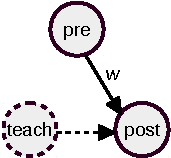
\includegraphics{pics_sdlm/ReSuMe.pdf} 
%	\end{minipage}
%	\begin{minipage}[c]{0.7\textwidth} 
%		\centering 
%		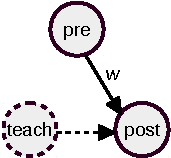
\includegraphics{pics_sdlm/resume.pdf} 
%	\end{minipage}
	\begin{subfigure}[c]{0.25\textwidth}
		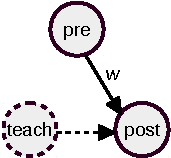
\includegraphics[width=\textwidth]{pics_sdlm/resume.pdf}
	\end{subfigure}
		\begin{subfigure}[c]{0.7\textwidth}
			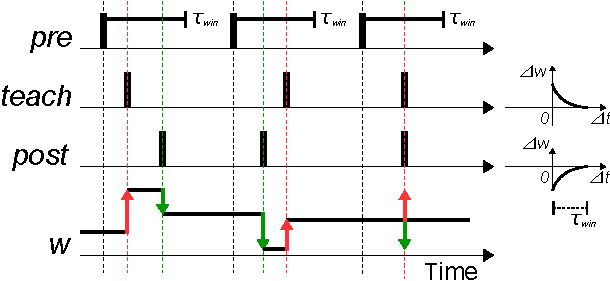
\includegraphics[width=\textwidth]{pics_sdlm/resume2.pdf}
		\end{subfigure}
	\caption{A pair of pre- and post-synaptic neurons trained by ReSuMe~\citep{ponulak2010supervised} with a teaching signal.}
	\label{fig:resume}
\end{figure}

The basic idea of the proposed method is to provide \DIFaddbegin \DIFadd{an }\DIFaddend equivalent learning rule as ReSuMe on rate-encoded SNNs.
The objective is to supervise the post-synaptic neuron to fire at the frequency of the teaching spike train. 
Accordingly, the weight decreases if the output neuron fires stronger than the teaching neuron, and vice versa.
The synaptic strength stops changing as the output neuron fires at the same frequency \DIFdelbegin \DIFdel{of }\DIFdelend \DIFaddbegin \DIFadd{as }\DIFaddend the teaching signal.
In the following section, we will firstly \DIFdelbegin \DIFdel{demonstrate how this idea was derived to mathematical descriptions of a }\DIFdelend \DIFaddbegin \DIFadd{describe this idea mathematically using the proposed term SRM, and equip learning to the method by }\DIFaddend biological-plausible \DIFdelbegin \DIFdel{learning rule, STDP }\DIFdelend \DIFaddbegin \DIFadd{STDP rule}\DIFaddend .
%The algorithm is simply divided into spike-based rate multiplication (SRM) problems, and we will demonstrate the SRM method in following Section~\ref{sec:SRM}.
%The learning rule can be easily applied to SAEs if we use input spikes as teaching signals to the visible units, moreover the CD algorithm of training SRBMs is still not more than two operations of SRMs.
%Section~\ref{sec:dSNN} explains the specific training on SAEs and SRBMs in detail.


\section{Spike-based Rate Multiplication (SRM)}
\label{sec:SRM}
\begin{figure}
	\centering
	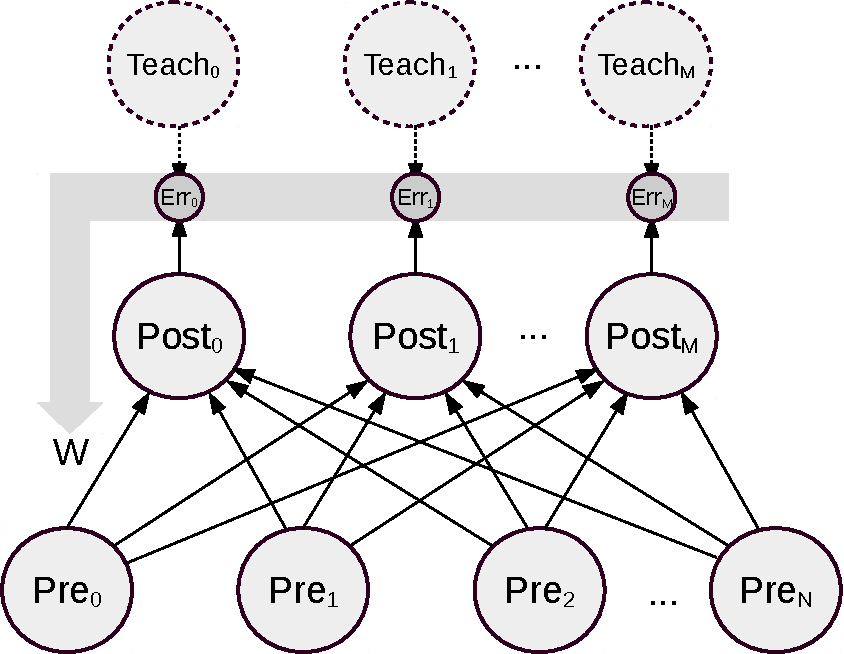
\includegraphics[width=0.6\textwidth]{pics_sdlm/adaline.pdf}
	\caption{The architecture of a single-layered network, ADALINE.}
	\label{fig:adaline}
\end{figure}
If we see \textit{pre}, \textit{post} and \textit{teach} as vectors individually, and \textit{w} as a weight matrix of the all-to-all connections between \textit{pre} and \textit{post} in Figure~\ref{fig:resume}, the network will form the ADALINE (Adaptive Linear Element) which is a single-layered ANN, see Figure~\ref{fig:adaline}.
The `Post' neurons perform \DIFaddbegin \DIFadd{a }\DIFaddend weighted sum on the input data, and the error between their output and the teaching data \DIFdelbegin \DIFdel{are }\DIFdelend \DIFaddbegin \DIFadd{is }\DIFaddend propagated to update the weights, thus to train the network to generate \DIFaddbegin \DIFadd{the }\DIFaddend same output as the \DIFdelbegin \DIFdel{teachers'}\DIFdelend \DIFaddbegin \DIFadd{teacher's}\DIFaddend . 
The learning algorithm was named after the researcher Widrow-Hoff:
\begin{equation}
\Delta w = \eta (teach - post)pre~.
\label{equ:widrow-hoff}
\end{equation}
%which is equivalent to Stochastic Gradient Descent~(SGD) in Multi-Layered Perceptrons~(MLPs).
The right hand \DIFaddbegin \DIFadd{side }\DIFaddend of the equation can be seen as a subtraction of two multiplication operations, $teach \times pre$ and $post \times pre$, times a learning rate, $\eta$.

SRM provides the solution to present numeric multiplication $c=ab$ with rate-based spike trains.
Firstly, the multiplier $a$ and the multiplicand $b$ are encoded into Poisson spike trains $s_a(t)=\{s_a(1),s_a(2),...,s_a(T)\}$ and $s_b(t)=\{s_b(1),s_b(2),...,s_b(T)\}$ \DIFdelbegin \DIFdel{in the }\DIFdelend \DIFaddbegin \DIFadd{with }\DIFaddend 1~ms resolution, where $s(t)=1$ indicates a spike in the $t$th~ms and $s(t)=0$ means \DIFdelbegin \DIFdel{none}\DIFdelend \DIFaddbegin \DIFadd{no spike}\DIFaddend .
Secondly, a Poisson generator fires a sequence of \DIFdelbegin \DIFdel{spike train }\DIFdelend \DIFaddbegin \DIFadd{spikes }\DIFaddend according to its firing rate, $\lambda$~Hz, which is assigned linearly to the original multiplier/multiplicand by a factor of $K$.
Hence, the firing rate ($\lambda_x$) of the Poisson generator is $K$ times the numerical value x, and can be approximated by the \DIFdelbegin \DIFdel{averaging }\DIFdelend \DIFaddbegin \DIFadd{average }\DIFaddend spike count, $N_T(s_x)$, of the generated spike train $s_x(t)$ over time \DIFdelbegin \DIFdel{length of }\DIFdelend $T$~ms:
\begin{equation}
\lambda_x = Kx \approx N_T(s_x) = \frac{1000}{T} \sum\DIFdelbegin \DIFdel{_{t=1}}\DIFdelend \DIFaddbegin \DIFadd{_{t=0}}\DIFaddend ^{T} s_x(t)~,
\end{equation} 
1000 is the scale factor to transfer frequency per millisecond to frequency per second.
Significantly, the approximation is more accurate as the observing time ($T$) grows since more spikes are generated over time and the \DIFdelbegin \DIFdel{averaging }\DIFdelend \DIFaddbegin \DIFadd{average }\DIFaddend spike count becomes more reliable.
Thirdly, assuming $s_a(t)$ and $s_b(t)$ are independent Poisson spike trains the core definition of the rate multiplication of the pair of spike trains is as follows:
\begin{equation}
\lambda_a \lambda_b \approx N_{T_1}(s_a)N_{T_2}(s_b)= 10^6 \frac{\sum_{t_a=1}^{T_1}s_a(t_a)}{T_1}  \frac{\sum_{t_b=1}^{T_2} s_b(t_b)}{T_2}~.
\label{equ:mul}
\end{equation} 

Finally, if we combine the concept of the STDP learning window \DIFdelbegin \DIFdel{to }\DIFdelend \DIFaddbegin \DIFadd{with }\DIFaddend equation~\ref{equ:mul}, the length of the observing time on $s_b$ shrinks to a fixed-length windowing period, \DIFdelbegin \DIFdel{$\tau_{win}$}\DIFdelend \DIFaddbegin \DIFadd{$\tau_{\textit{\textrm{win}}}$}\DIFaddend .
Consequently, the rate multiplication can be conducted within only the local events in \DIFdelbegin \DIFdel{term }\DIFdelend \DIFaddbegin \DIFadd{terms }\DIFaddend of time, although the accuracy may drop.
The rate multiplication is then approximated by:
\begin{equation}
\lambda_a \lambda_b \approx \DIFdelbegin \DIFdel{\frac{10^6}{\tau_{dur} \tau_{win}} }\DIFdelend \DIFaddbegin \DIFadd{\frac{10^6}{\tau_{\textit{\textrm{dur}}} \tau_{\textit{\textrm{win}}}} }\DIFaddend \sum\DIFdelbegin \DIFdel{_{t=1}^{\tau_{dur}} }\DIFdelend \DIFaddbegin \DIFadd{_{t=0}^{\tau_{\textit{\textrm{dur}}}} }\DIFaddend [s_a(t) \sum_{t_b=t}\DIFdelbegin \DIFdel{^{t+\tau_{win}} }\DIFdelend \DIFaddbegin \DIFadd{^{t+\tau_{\textit{\textrm{win}}}} }\DIFaddend s_b(t_b)]~,
\end{equation} 
where \DIFdelbegin \DIFdel{$\tau_{dur}$ }\DIFdelend \DIFaddbegin \DIFadd{$\tau_{\textit{\textrm{dur}}}$ }\DIFaddend replaces $T$ to represent the length of generated spike trains during SNN simulation.
The weight rise/drop according to a rectangular STDP curve can detect the spike events of a pair of neurons when a post-synaptic spike occurs \DIFaddbegin \DIFadd{coincidently (}\DIFaddend no later than \DIFdelbegin \DIFdel{$\tau_{win}$}\DIFdelend \DIFaddbegin \DIFadd{$\tau_{\textit{\textrm{win}}}$)}\DIFaddend , see Figure~\ref{fig:rtg_stdp}.
Therefore, the overall weight change during time \DIFdelbegin \DIFdel{$\tau_{dur}$ indicates }\DIFdelend \DIFaddbegin \DIFadd{$\tau_{\textit{\textrm{dur}}}$ is determined by the number of coincident spikes of the pair of neurons, indicating }\DIFaddend the rate multiplication, and is \DIFdelbegin \DIFdel{descried }\DIFdelend \DIFaddbegin \DIFadd{described }\DIFaddend by SRM:
\begin{equation}
\begin{aligned}
\Delta w = SRM(s_a, s_b) &= \eta_s \sum\DIFdelbegin \DIFdel{_{t=1}^{\tau_{dur}} }\DIFdelend \DIFaddbegin \DIFadd{_{t=0}^{\tau_{\textit{\textrm{dur}}}} }\DIFaddend [s_a(t) \sum_{t_b=t}\DIFdelbegin \DIFdel{^{t+\tau_{win}} }\DIFdelend \DIFaddbegin \DIFadd{^{t+\tau_{\textit{\textrm{win}}}} }\DIFaddend s_b(t_b)] \text{~,~and}\\
c=ab=\frac{\lambda_a \lambda_b}{K^2} &\approx \DIFdelbegin \DIFdel{\frac{10^6}{K^2 \tau_{dur} \tau_{win}} }\DIFdelend \DIFaddbegin \DIFadd{\frac{10^6}{K^2 \tau_{\textit{\textrm{dur}}} \tau_{\textit{\textrm{win}}}} }\DIFaddend \sum\DIFdelbegin \DIFdel{_{t=1}^{\tau_{dur}} }\DIFdelend \DIFaddbegin \DIFadd{_{t=0}^{\tau_{\textit{\textrm{dur}}}} }\DIFaddend [s_a(t) \sum_{t_b=t}\DIFdelbegin \DIFdel{^{t+\tau_{win}} }\DIFdelend \DIFaddbegin \DIFadd{^{t+\tau_{\textit{\textrm{win}}}} }\DIFaddend s_b(t_b)] \\
&\approx  \DIFdelbegin \DIFdel{\frac{10^6 SRM(s_a, s_b)}{K^2 \tau_{dur} \tau_{win}  \eta_s}}\DIFdelend \DIFaddbegin \DIFadd{\frac{10^6 SRM(s_a, s_b)}{K^2 \tau_{\textit{\textrm{dur}}} \tau_{\textit{\textrm{win}}}  \eta_s}}\DIFaddend ~.
\end{aligned}
\label{equ:srm}
\end{equation} 
\begin{figure}
	\centering
	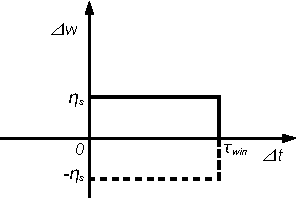
\includegraphics[width=0.4\textwidth]{pics_sdlm/stdp.pdf}
	\caption{Rectangular STDP curve.
		If the time difference \DIFdelbeginFL \DIFdelFL{of }\DIFdelendFL \DIFaddbeginFL \DIFaddFL{between }\DIFaddendFL the post-synaptic spike and the pre-synaptic spike lies in the window \DIFdelbeginFL \DIFdelFL{on $\tau_{win}$}\DIFdelendFL \DIFaddbeginFL \DIFaddFL{$\tau_{\textit{\textrm{win}}}$}\DIFaddendFL , then the synaptic weight will increase or decrease by $\eta_s$ according to the sign of the SRM.}
	\label{fig:rtg_stdp}
\end{figure}

We can adjust $\eta_s$ to \DIFdelbegin \DIFdel{$ K^2 \tau_{dur} \tau_{win}10^{-6}$ }\DIFdelend \DIFaddbegin \DIFadd{$ K^2 \tau_{\textit{\textrm{dur}}} \tau_{\textit{\textrm{win}}}10^{-6}$ }\DIFaddend to make $ab = \Delta w$.
In terms of the Widrow-Hoff learning algorithm, $\eta_s$ is set to be:
\begin{equation}
	\eta_s=
    \left\{
    \begin{aligned} 
    \eta K^2 \tau\DIFdelbegin \DIFdel{_{dur} }\DIFdelend \DIFaddbegin \DIFadd{_{\textit{\textrm{dur}}} }\DIFaddend \tau\DIFdelbegin \DIFdel{_{win}}\DIFdelend \DIFaddbegin \DIFadd{_{\textit{\textrm{win}}}}\DIFaddend 10^{-6}, &\text{ when calculating } \eta teach \times pre\\
    - \eta K^2 \tau\DIFdelbegin \DIFdel{_{dur} }\DIFdelend \DIFaddbegin \DIFadd{_{\textit{\textrm{dur}}} }\DIFaddend \tau\DIFdelbegin \DIFdel{_{win}}\DIFdelend \DIFaddbegin \DIFadd{_{\textit{\textrm{win}}}}\DIFaddend 10^{-6}, &\text{ when calculating } \eta post \times pre
    \end{aligned}
    \right.
    \label{equ:eta_s}
\end{equation}
%DIF < In Section~\ref{sec:AE}, we demonstrate how Widrow-Hoff algorithm successfully is applied to training AEs (see Equation~\ref{equ:ae_widrow_hoff}) and in Section~\ref{subsec:SAE} we describe the implementation of SRM algorithm to deep learning models of spiking AEs and RBMs.
%DIF > In Section~\ref{sec:AE}, we demonstrate how Widrow-Hoff algorithm successfully is applied to training AEs (see Equation~\ref{equ:ae_widrow_hoff}) and in Section~\ref{subsec:SAE} we describe the implementation of SRM algorithm to Deep Learning models of spiking AEs and RBMs.

Last but not least, we state the property of \DIFaddbegin \DIFadd{the }\DIFaddend SRM algorithm:
\begin{itemize}
	\item the accuracy of SRM is mainly controlled by \DIFdelbegin \DIFdel{$\tau_{dur}$ and $\tau_{win}$}\DIFdelend \DIFaddbegin \DIFadd{$\tau_{\textit{\textrm{dur}}}$ and $\tau_{\textit{\textrm{win}}}$}\DIFaddend , where longer spike trains and a longer STDP window expresses the rate more \DIFdelbegin \DIFdel{reliable}\DIFdelend \DIFaddbegin \DIFadd{reliably}\DIFaddend .
	\item in our spiking neural network both the multiplier and the multiplicand can be presented only as rates, which are positive quantities.
	Thus \DIFaddbegin \DIFadd{a }\DIFaddend negative product is applied with weight decrease, $-\eta_s$. 
	\item the multiplier and the multiplicand are interchangeable due to the independence of the spike trains. 
	\item the accuracy is independent of \DIFaddbegin \DIFadd{the }\DIFaddend neural and synaptic \DIFdelbegin \DIFdel{model of a }\DIFdelend \DIFaddbegin \DIFadd{models of the }\DIFaddend spiking neuron because the calculation relies on the firing rate only.
\end{itemize}


\section{Training Deep SNNs}
\label{sec:dSNN}
Following the idea of supervising a spike-based, single-layered ADALINE network by STDP learning, we then seek solutions for training deep neural architectures.
In Sections~\ref{sec:AE} and \ref{sec:rbm}, we \DIFdelbegin \DIFdel{have }\DIFdelend derived the training algorithms of AEs and RBMs in detail, whose learning rules are of \DIFaddbegin \DIFadd{the }\DIFaddend same structure as Widrow-Hoff~(Equation~\ref{equ:widrow-hoff}) for ADALINE, see Equations~\ref{equ:ae_widrow_hoff} and~\ref{equ:rbm_train}.
Consequently, we can easily apply SRM in training spiking AEs and RBMs and conduct experiments to compare conventional \DIFdelbegin \DIFdel{deep learning }\DIFdelend \DIFaddbegin \DIFadd{Deep Learning }\DIFaddend modules with the spiking versions.

\begin{figure}
	\centering
	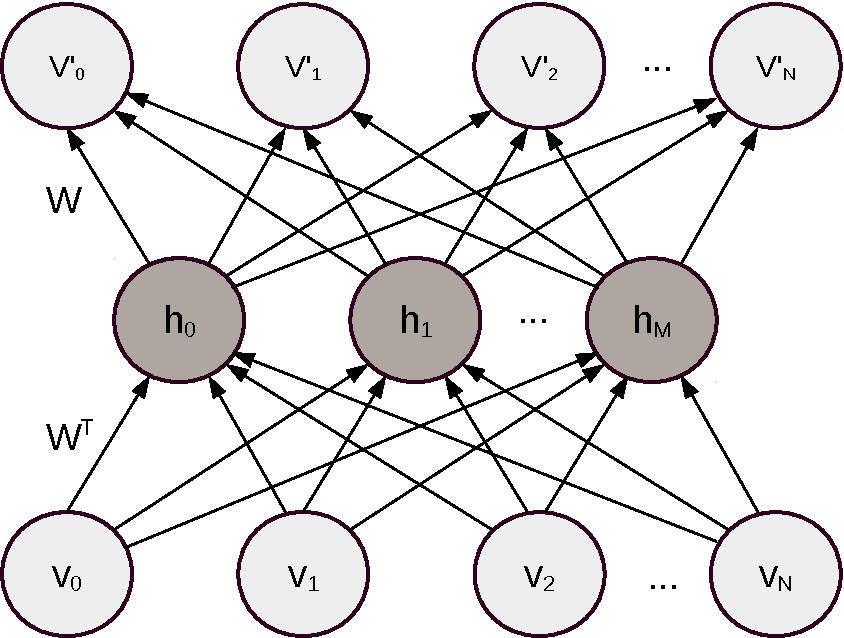
\includegraphics[width=0.5\textwidth]{pics_sdlm/AE.pdf}
	\caption{Symmetric weights connected between visible ($\bf{v}$) and hidden ($\bf{h}$) units in AEs and RBMs to reconstruct visible inputs, $\bf{v'}$.}
	\label{fig:sym_conn}
\end{figure}
Initially, AEs and RBMs were trained with clean numerical values, then with noisy values generated by counting \DIFdelbegin \DIFdel{spikes of }\DIFdelend \DIFaddbegin \DIFadd{the spikes in }\DIFaddend Poisson spike trains.
%presenting the original values with Poisson spike trains and transferring the spike counts back to numerical values.
There were two set-ups of the same network architecture~(Figure~\ref{fig:sym_conn}) where ten visible neurons connected to a layer of ten hidden neurons symmetrically with all-to-all weights: In Experiment~1 (Exp1), the values of all the input data were 1, $input_1 = [1, 1, 1,...,1]$; and in Experiment~2 (Exp2), the input data ranged from 0.1 to 1 linearly with steps of 0.1, $input_2 = [0.1, 0.2, 0.3,...,1]$.
These two experiments provided a close observation on the dynamic weight change given constant inputs.
Exp1 shows how the network responded to the same input value and reconstructed it, while Exp2 demonstrated the influence of ranging input values and more importantly how different firing \DIFdelbegin \DIFdel{rate }\DIFdelend \DIFaddbegin \DIFadd{rates }\DIFaddend may affect the corresponding SNN.
These experiments were run as baselines to compare with spike-based training on the features of \DIFdelbegin \DIFdel{weights' }\DIFdelend \DIFaddbegin \DIFadd{weight }\DIFaddend convergence, reconstruction error and \DIFdelbegin \DIFdel{neurons' }\DIFdelend \DIFaddbegin \DIFadd{neural }\DIFaddend activities.

Following the experiments on conventional models, we propose the training methods for SAEs and SRBMs in detail.
The same experiments were then applied to the on-line and spike-based SNN training.

\subsection{Autoencoders (AEs)}
\label{sec:ae}
Using ReLU and Equation~\ref{equ:ae_widrow_hoff}, we can easily train a layer of AEs with a small network size of 10 visible units and 10 output units.
The initial weights were randomly generated with unified distribution from 0 to 0.01 and the learning rate, $\eta$, is set to 0.001.
We kept the same initial weights for all the experiments thus providing an accurate comparison on the weight updates.
The input vector, seen as an image, repeatedly fed into the network $5,000$ times and Figure~\ref{fig:ae_orig} shows the dynamics of the AE as more repeating images \DIFdelbegin \DIFdel{present }\DIFdelend \DIFaddbegin \DIFadd{are presented }\DIFaddend through training.

\begin{figure}
	\centering
	\begin{subfigure}[t]{0.45\textwidth}
		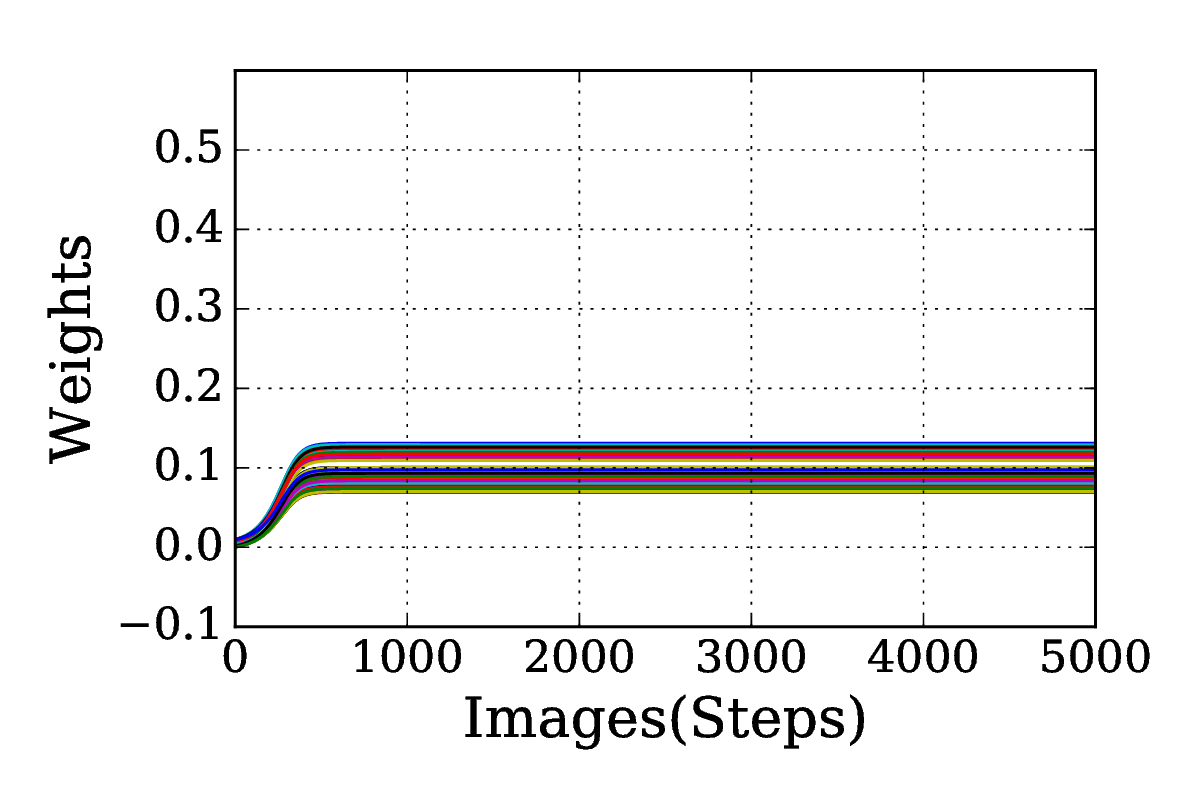
\includegraphics[width=\textwidth]{pics_sdlm/20_exp_AE/exp1_weights_non.png}
		\caption{Weights of Exp1}
	\end{subfigure}
	\begin{subfigure}[t]{0.45\textwidth}
		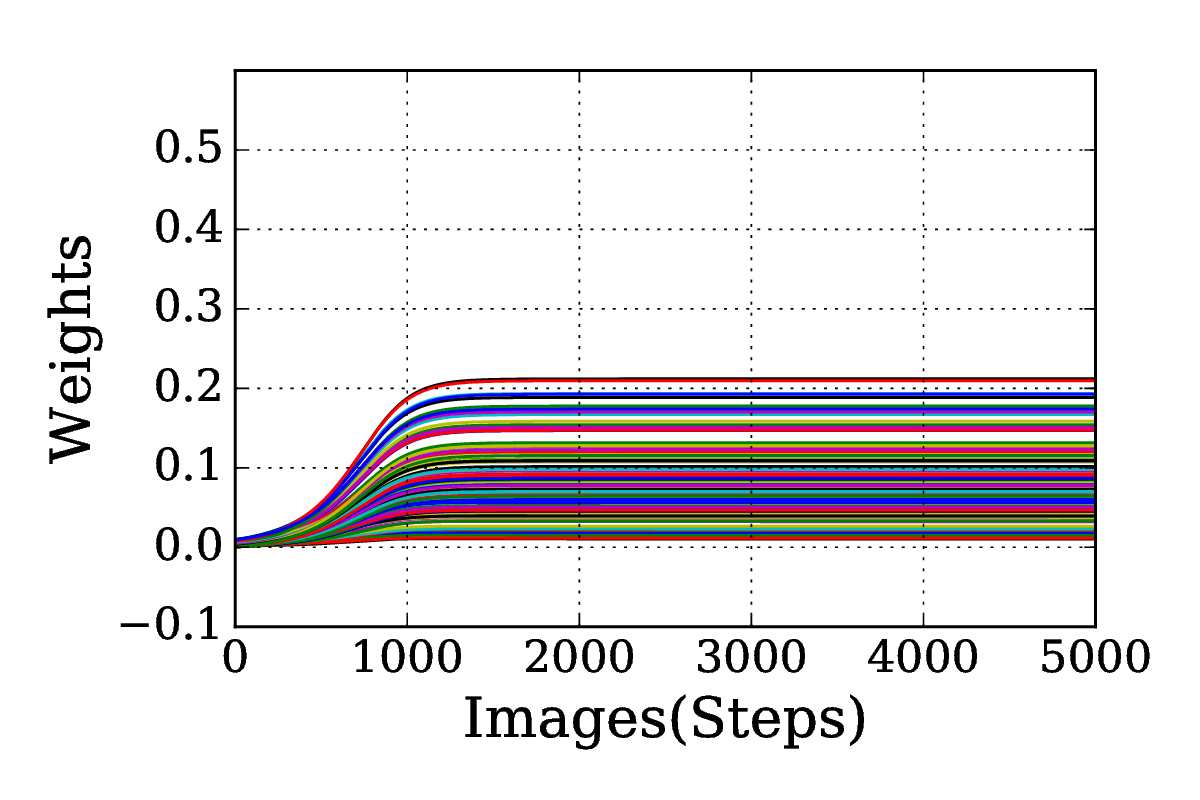
\includegraphics[width=\textwidth]{pics_sdlm/20_exp_AE/exp2_weights_non.png}
		\caption{Weights of Exp2}
	\end{subfigure}
	\begin{subfigure}[t]{0.45\textwidth}
		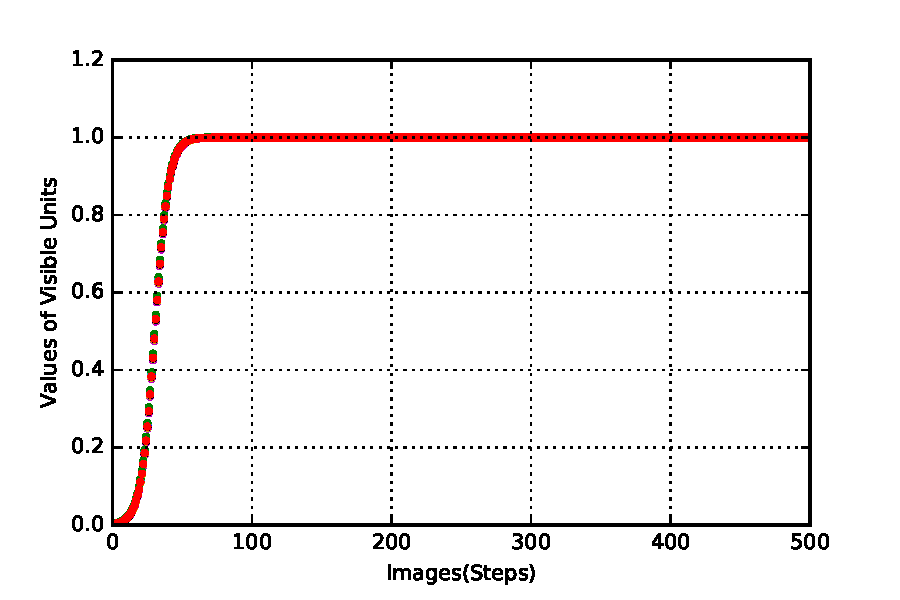
\includegraphics[width=\textwidth]{pics_sdlm/20_exp_AE/exp1_recon_non.pdf}
		\caption{Reconstruction of visible units in Exp1}
	\end{subfigure}
	\begin{subfigure}[t]{0.45\textwidth}
		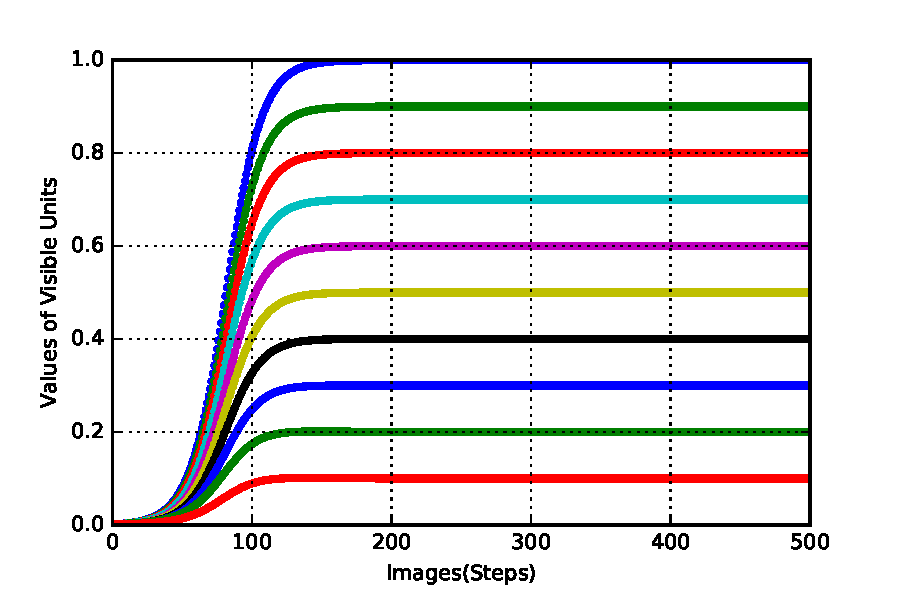
\includegraphics[width=\textwidth]{pics_sdlm/20_exp_AE/exp2_recon_non.pdf}
		\caption{Reconstruction of visible units in Exp2}
	\end{subfigure}\\
	\begin{subfigure}[t]{0.45\textwidth}
		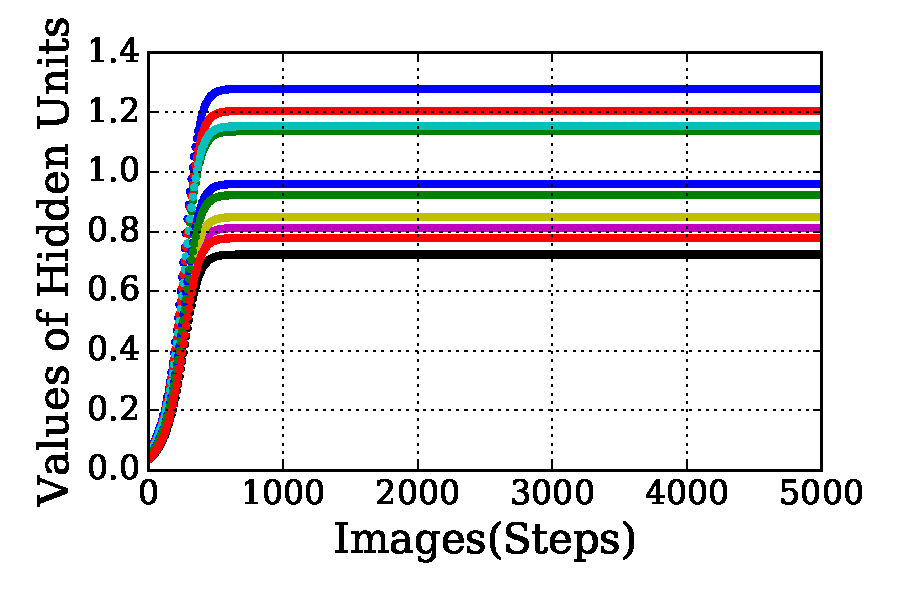
\includegraphics[width=\textwidth]{pics_sdlm/20_exp_AE/exp1_hid_non.pdf}
		\caption{Output of hidden units in Exp1}
	\end{subfigure}
	\begin{subfigure}[t]{0.45\textwidth}
		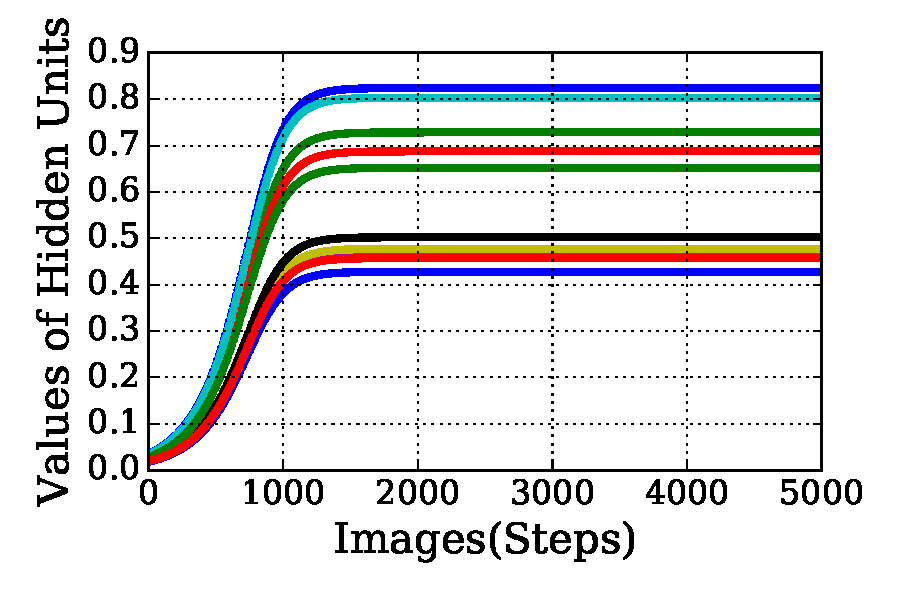
\includegraphics[width=\textwidth]{pics_sdlm/20_exp_AE/exp2_hid_non.pdf}
		\caption{Output of hidden units in Exp2}
	\end{subfigure}\\
	\begin{subfigure}[t]{0.45\textwidth}
		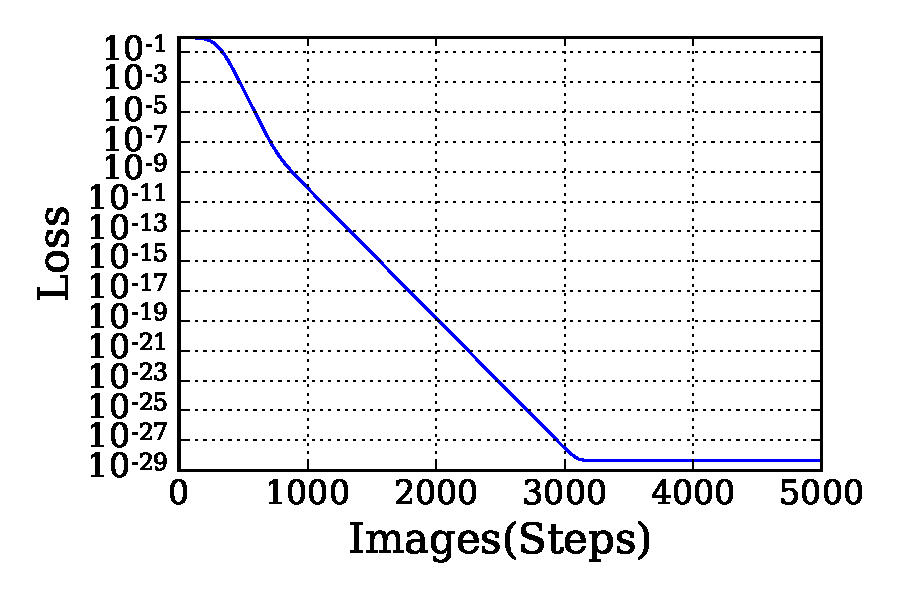
\includegraphics[width=\textwidth]{pics_sdlm/20_exp_AE/exp1_loss.pdf}
		\caption{Output of hidden units in Exp1}
	\end{subfigure}
	\begin{subfigure}[t]{0.45\textwidth}
		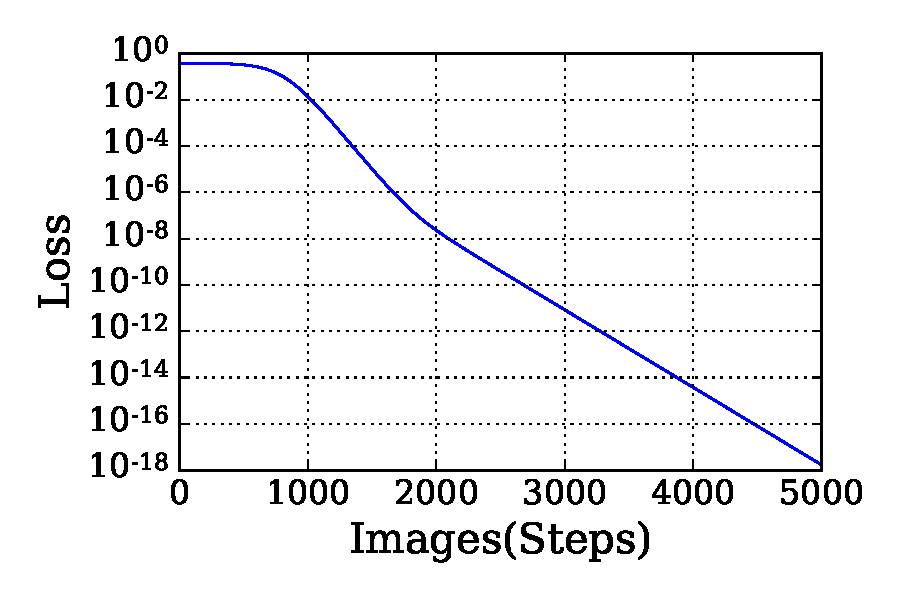
\includegraphics[width=\textwidth]{pics_sdlm/20_exp_AE/exp2_loss.pdf}
		\caption{Output of hidden units in Exp2}
	\end{subfigure}
	\caption{Changes of weights, output of visible and hidden units, and mean squared error (loss) during the AE training of the reconstruction tests. 
		Experiments 1) 10 visible units fully connected to 10 hidden units with input data of all 1s; 2) \DIFaddbeginFL \DIFaddFL{the }\DIFaddendFL same network fed with 10 values \DIFdelbeginFL \DIFdelFL{distribute }\DIFdelendFL \DIFaddbeginFL \DIFaddFL{distributed }\DIFaddendFL linearly from 0.1 to 1.}
	\label{fig:ae_orig}
\end{figure}

To compare all the following experiments, we present the results in the same template of figures:
among such a set of figures, (a) and (b) depict the weight \DIFdelbegin \DIFdel{change }\DIFdelend \DIFaddbegin \DIFadd{changes }\DIFaddend of the two experiment set-ups (Exp1 and Exp2) which \DIFdelbegin \DIFdel{is }\DIFdelend \DIFaddbegin \DIFadd{are }\DIFaddend the most important output of \DIFdelbegin \DIFdel{a }\DIFdelend \DIFaddbegin \DIFadd{the }\DIFaddend training method;
(c) and (d) display the output of the visible units, the reconstruction of the input vector;
(e) and (f) draw the output of the hidden units during training and assist the observation on weight change and the reconstruction;
(g) and (h) intuitively show the loss (mean squared error) and validate the accuracy of the reconstructions.


For Exp1, the reconstruction loss reduced exponentially to the limit of the computer's float precision (Figure~\ref{fig:ae_orig}(g)), and reached $10^{-4}$ using about 600 steps, and from that point the weights, visible reconstruction, and the output of the hidden units nearly stabilised, see Figure~\ref{fig:ae_orig}(a,c,e).
With different input values of Exp2, the training ran slower taking about $1,400$ steps to reached the same performance of $10^{-4}$ loss (Figure~\ref{fig:ae_orig}(h)).
The reason for the slower training was due to the weaker input which also resulted in lower output of the hidden units comparing to Exp1, see Figure~\ref{fig:ae_orig}(f), so that the positive part of the weight change, $\eta h_i v_j$, was much weakened. 
The reconstructions, shown in Figure~\ref{fig:ae_orig}(d), of smaller values stabilised earlier than the ones of higher values, since the higher output of the reconstruction required stronger weights and more accumulated weight updates. 
\begin{figure}
	\centering
	\begin{subfigure}[t]{0.45\textwidth}
		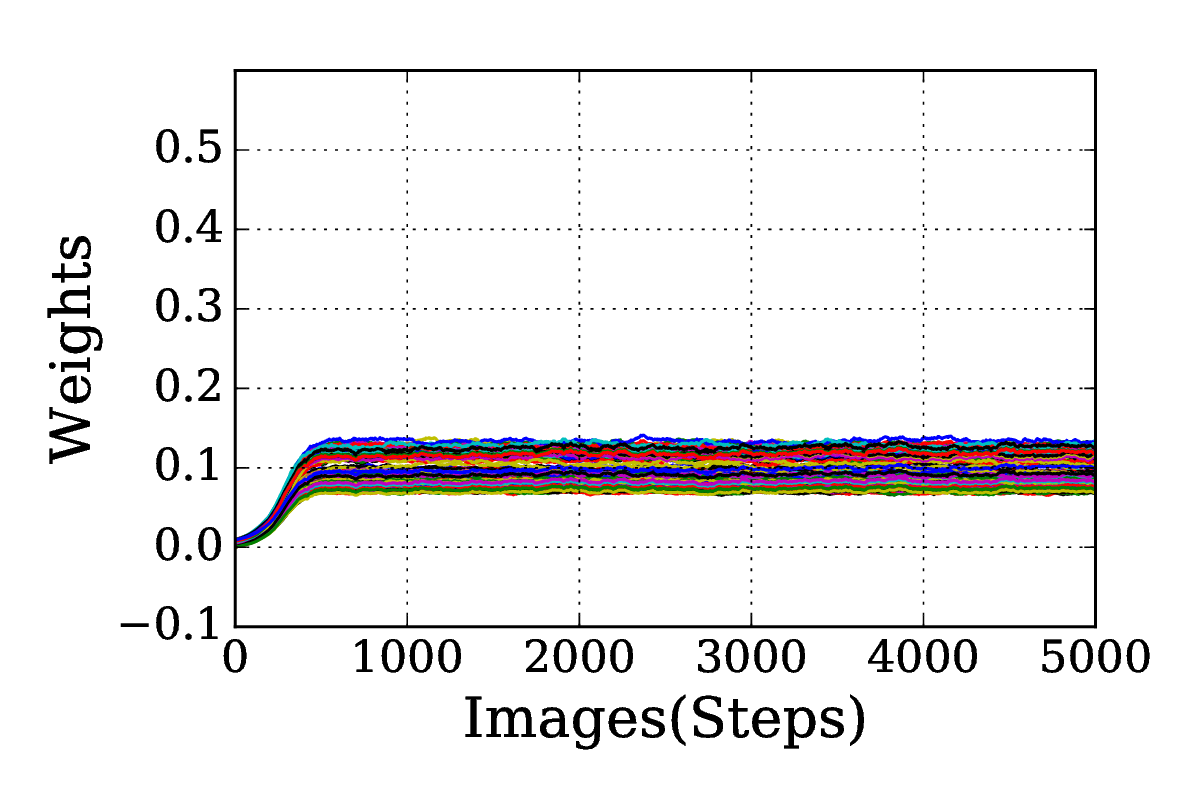
\includegraphics[width=\textwidth]{pics_sdlm/21_exp_AE_noise/exp1_weights_s.png}
		\caption{Weights of Exp1}
	\end{subfigure}
	\begin{subfigure}[t]{0.45\textwidth}
		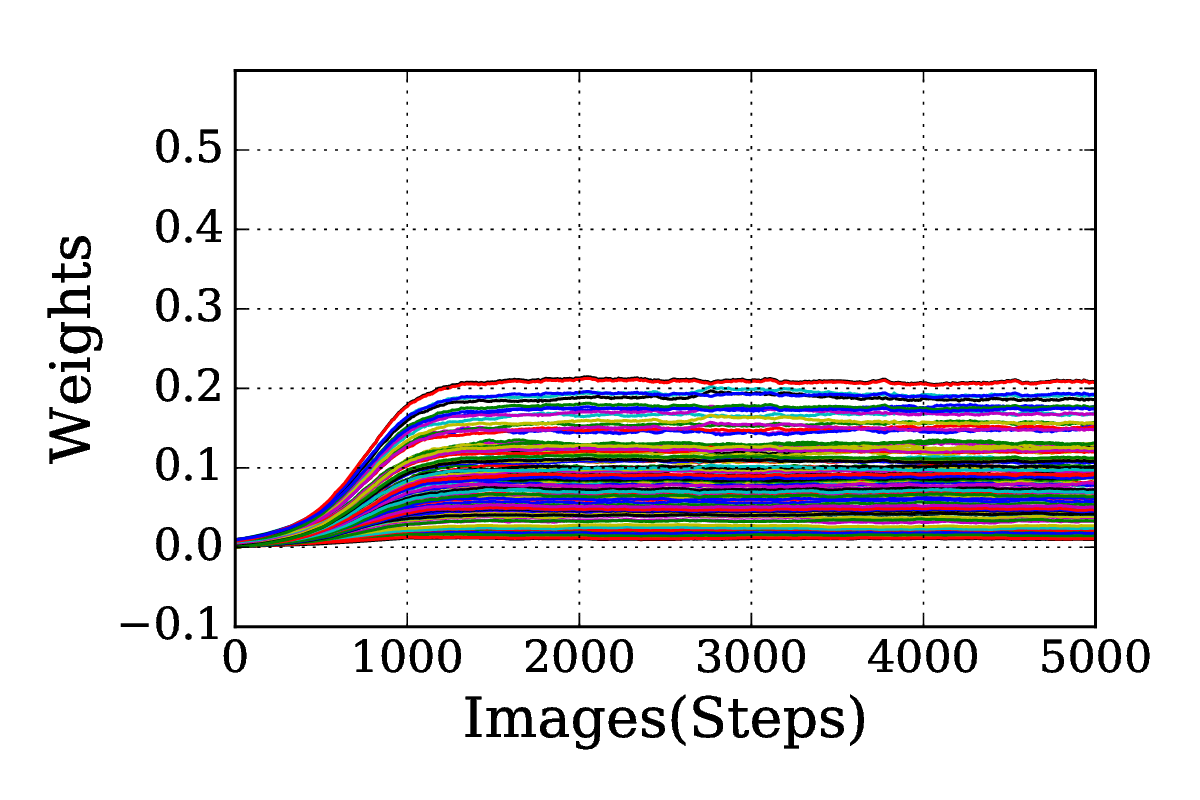
\includegraphics[width=\textwidth]{pics_sdlm/21_exp_AE_noise/exp2_weights_s.png}
		\caption{Weights of Exp2}
	\end{subfigure}
	\begin{subfigure}[t]{0.45\textwidth}
		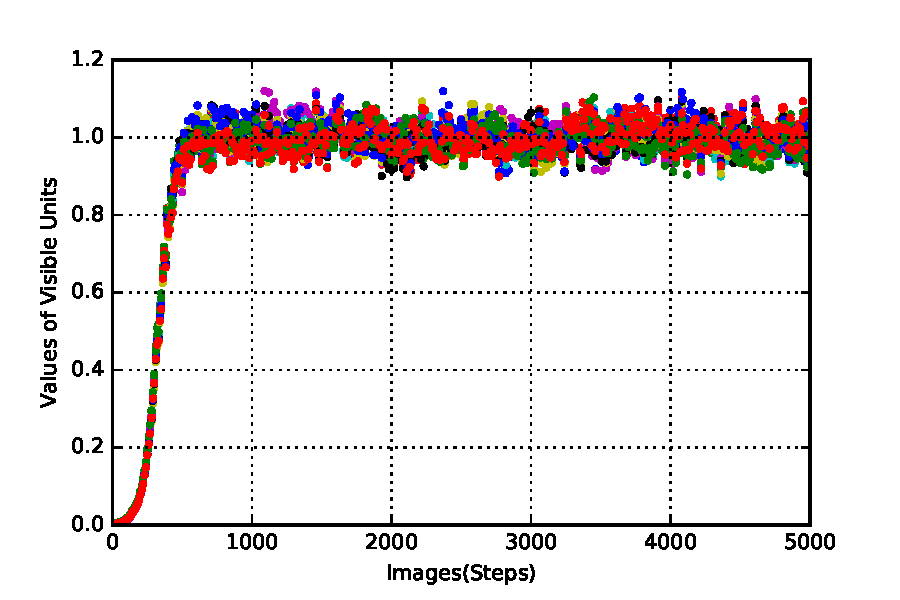
\includegraphics[width=\textwidth]{pics_sdlm/21_exp_AE_noise/exp1_recon_s.pdf}
		\caption{Reconstruction of visible units in Exp1}
	\end{subfigure}
	\begin{subfigure}[t]{0.45\textwidth}
		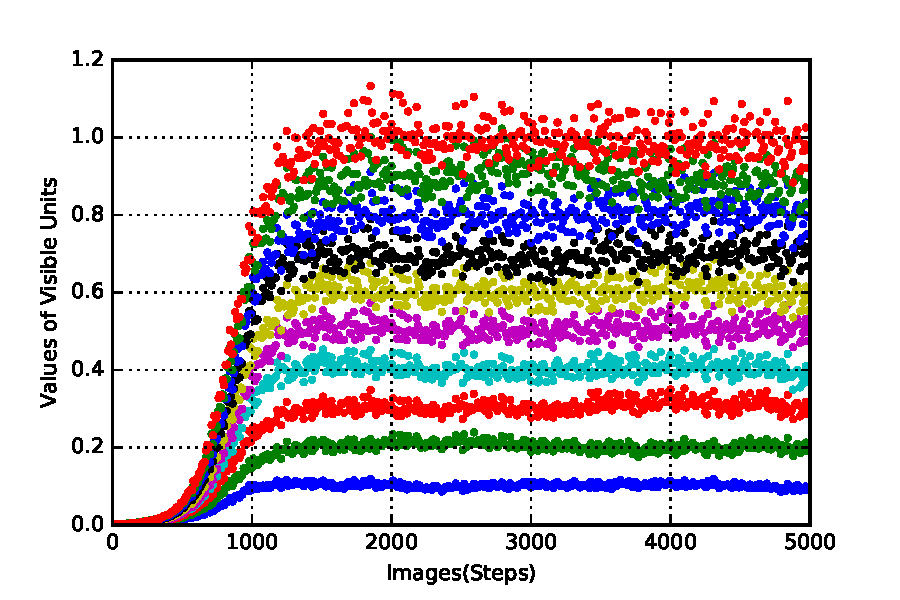
\includegraphics[width=\textwidth]{pics_sdlm/21_exp_AE_noise/exp2_recon_s.pdf}
		\caption{Reconstruction of visible units in Exp2}
	\end{subfigure}\\
	\begin{subfigure}[t]{0.45\textwidth}
		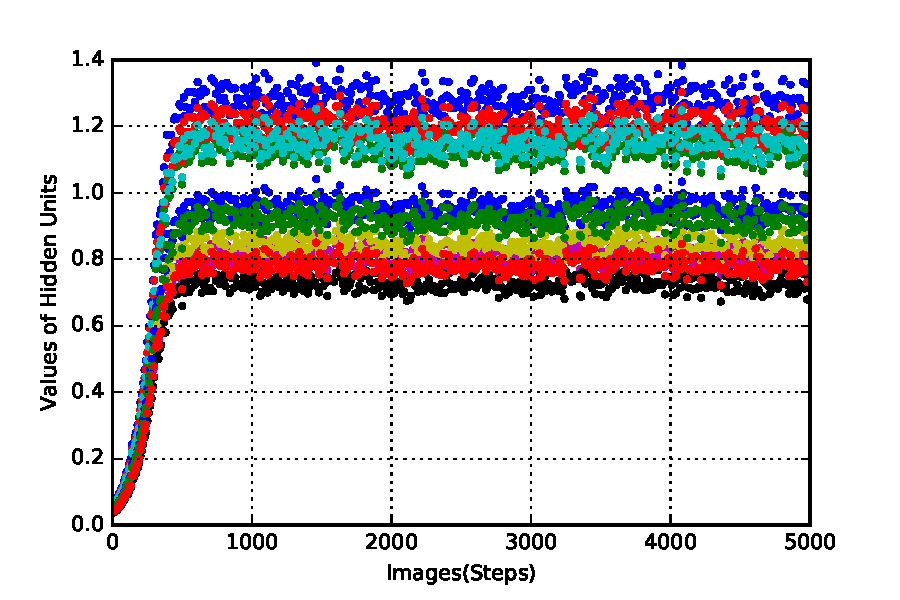
\includegraphics[width=\textwidth]{pics_sdlm/21_exp_AE_noise/exp1_hid_s.pdf}
		\caption{Output of hidden units in Exp1}
	\end{subfigure}
	\begin{subfigure}[t]{0.45\textwidth}
		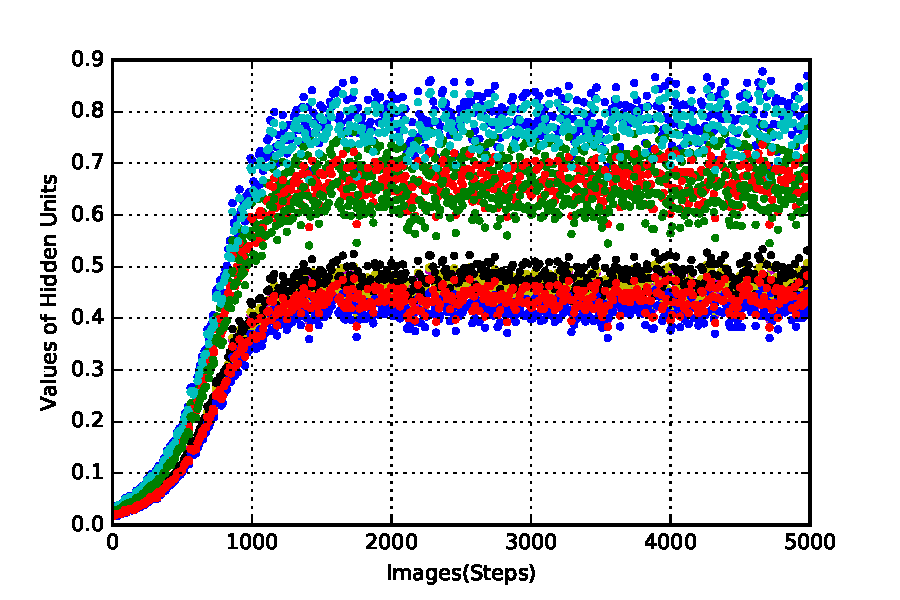
\includegraphics[width=\textwidth]{pics_sdlm/21_exp_AE_noise/exp2_hid_s.pdf}
		\caption{Output of hidden units in Exp2}
	\end{subfigure}\\
	\begin{subfigure}[t]{0.45\textwidth}
		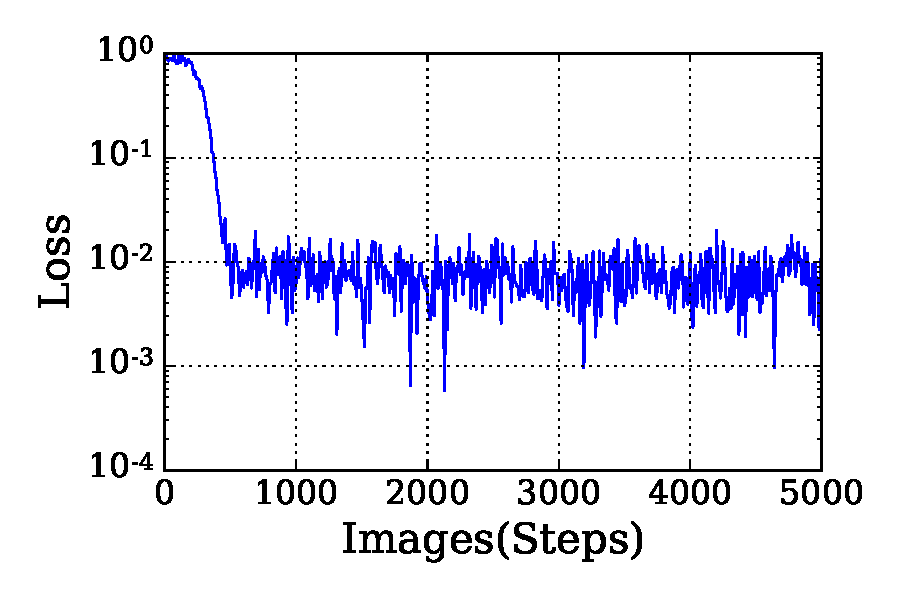
\includegraphics[width=\textwidth]{pics_sdlm/21_exp_AE_noise/exp1_loss_s.pdf}
		\caption{Output of hidden units in Exp1}
	\end{subfigure}
	\begin{subfigure}[t]{0.45\textwidth}
		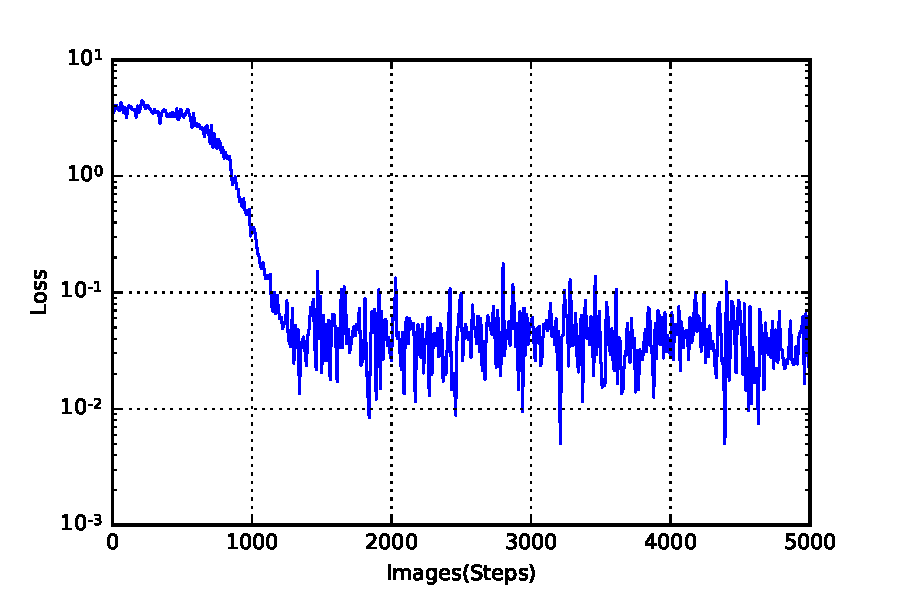
\includegraphics[width=\textwidth]{pics_sdlm/21_exp_AE_noise/exp2_loss_s.pdf}
		\caption{Output of hidden units in Exp2}
	\end{subfigure}
	\caption{Changes of weights, output of visible and hidden units, and mean squared error (loss) during the AE training of the noisy reconstruction tests. 
		Experiments 1) 10 visible units fully connected to 10 hidden units with the count of Poisson spikes firing at 100~Hz which lasted 100~ms; 2) \DIFaddbeginFL \DIFaddFL{the }\DIFaddendFL same network fed with spike count of Poisson spikes at firing \DIFdelbeginFL \DIFdelFL{rate }\DIFdelendFL \DIFaddbeginFL \DIFaddFL{rates }\DIFaddendFL ranging from 10~Hz to 100~Hz.}
	\label{fig:ae_noise}
\end{figure}

The same experiments were repeated with noisy training and testing data to provide a fair comparison with the spike-based \DIFdelbegin \DIFdel{deep learning }\DIFdelend \DIFaddbegin \DIFadd{Deep Learning }\DIFaddend modules, see Figure~\ref{fig:ae_noise}.
The noisy data was gathered from the SNN experiments in Section~\ref{subsec:SAE}, and the corresponding SRM parameters were listed in Table~\ref{tbl:srm}.
All the SNN experiments used the same training and testing Poisson spike trains for the purpose of the unified experimental environment.
The firing rates of the input values were scaled up by the factor $K = 100$, thus $\lambda_1 = [100, 100, 100, ..., 100]$ Hz and $\lambda_2 = [10, 20, 30, ..., 100]$ Hz.
The spike count \DIFdelbegin \DIFdel{$N_{\tau_{dur}}$ }\DIFdelend \DIFaddbegin \DIFadd{$N_{\tau_{\textit{\textrm{dur}}}}$ }\DIFaddend of the generated Poisson spike train then transformed to the noisy input, \DIFdelbegin \DIFdel{$N_{\tau_{dur}}*1000/(\tau_{dur} * K)$}\DIFdelend \DIFaddbegin \DIFadd{$N_{\tau_{\textit{\textrm{dur}}}}*1000/(\tau_{\textit{\textrm{dur}}} * K)$}\DIFaddend .
The scaling factor $1,000$ \DIFdelbegin \DIFdel{transfers }\DIFdelend \DIFaddbegin \DIFadd{converts }\DIFaddend ms to s, and the length of spike trains \DIFdelbegin \DIFdel{$\tau_{dur}$ }\DIFdelend \DIFaddbegin \DIFadd{$\tau_{\textit{\textrm{dur}}}$ }\DIFaddend was 100~ms when training, and $1,000$~ms for testing.
The longer the spike trains, the less noisy the spike counts become.
The noisy input can be seen as distorted data by adding Gaussian noise on the original value.
Hence, the noisy training input added to the clean data a Gaussian noise with -0.05 mean and 0.29 variance for Exp1, and -0.02 mean and 0.22 variance for Exp2;
while in terms of testing data, see Figure~\ref{fig:noise_input}, the means of the noise were the same, but the variances were much smaller: 0.09 for Exp1 and 0.07 for Exp2.
\begin{figure}
	\centering
	\begin{subfigure}[t]{0.45\textwidth}
		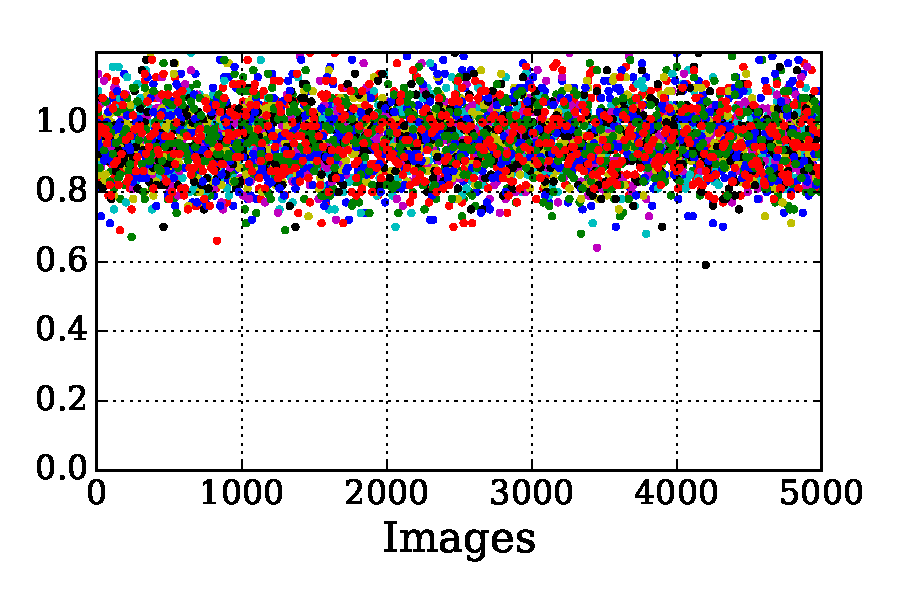
\includegraphics[width=\textwidth]{pics_sdlm/21_exp_AE_noise/exp1.pdf}
		\caption{Input values of Exp1}
	\end{subfigure}
	\begin{subfigure}[t]{0.45\textwidth}
		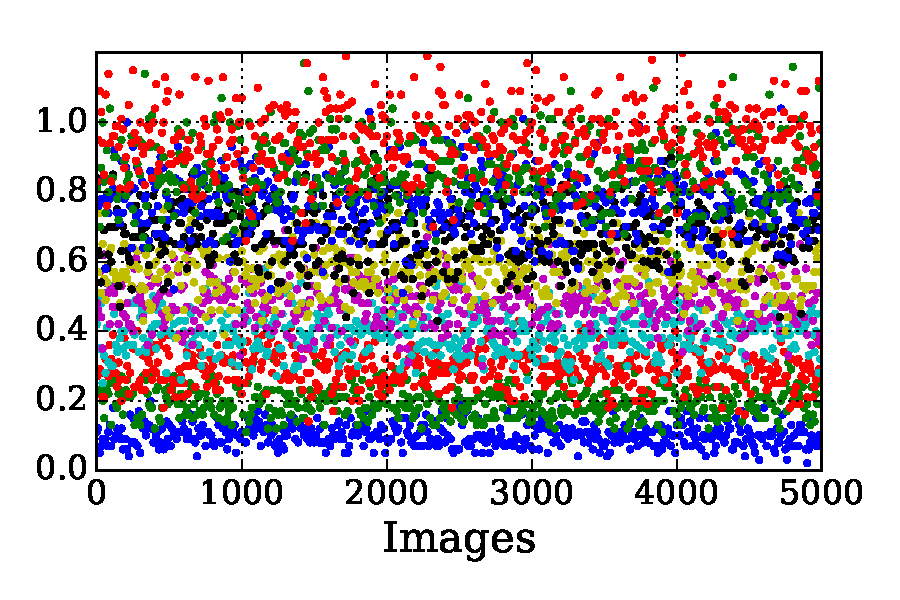
\includegraphics[width=\textwidth]{pics_sdlm/21_exp_AE_noise/exp2.pdf}
		\caption{Input values of Exp2}
	\end{subfigure}
	\caption{Noisy input gathered from Poisson spike trains.}
	\label{fig:noise_input}
\end{figure}


Figure~\ref{fig:ae_noise} shows the effect of the noisy input, although the training stabilised at roughly the same time point.
Firstly, it generated slight fluctuations on the weight change.
Secondly, the reconstruction and the output of the hidden units were noisy compared to the training and testing on clean data, however the noise was much reduced from the noisy input data (Figure~\ref{fig:noise_input}). 
Finally, the losses kept at a certain level and stopped dropping.
The loss in Exp2 was lower than Exp1, in other words the reconstruction on Exp2 were closer to the input data.
\DIFdelbegin \DIFdel{It }\DIFdelend \DIFaddbegin \DIFadd{This }\DIFaddend was mainly caused by the weaker noise level on the smaller input values which made the data of Exp2 less noisy \DIFdelbegin \DIFdel{in }\DIFdelend \DIFaddbegin \DIFadd{on }\DIFaddend average.
So was the reconstruction, which led to the lower level of loss.
\begin{figure}
	\centering
	\begin{subfigure}[t]{0.45\textwidth}
		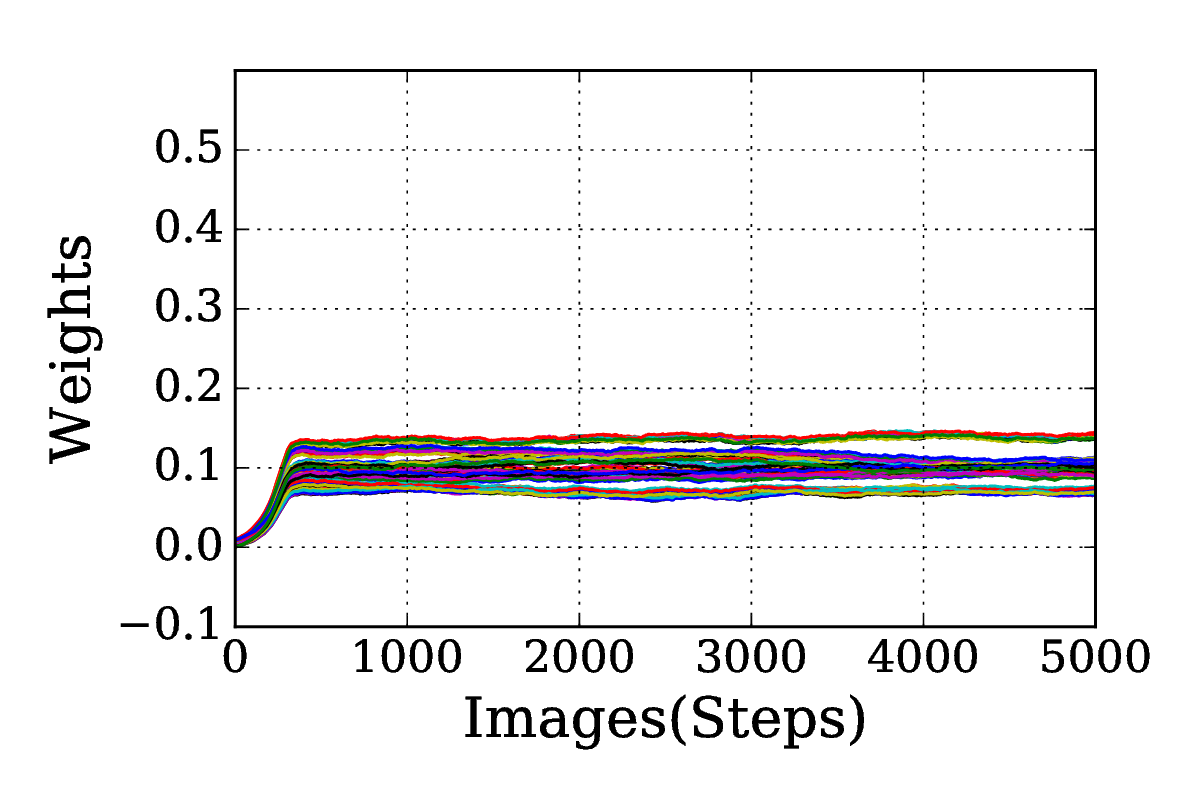
\includegraphics[width=\textwidth]{pics_sdlm/30_exp_RBM/exp1_weights_non.png}
		\caption{Weights of Exp1}
	\end{subfigure}
	\begin{subfigure}[t]{0.45\textwidth}
		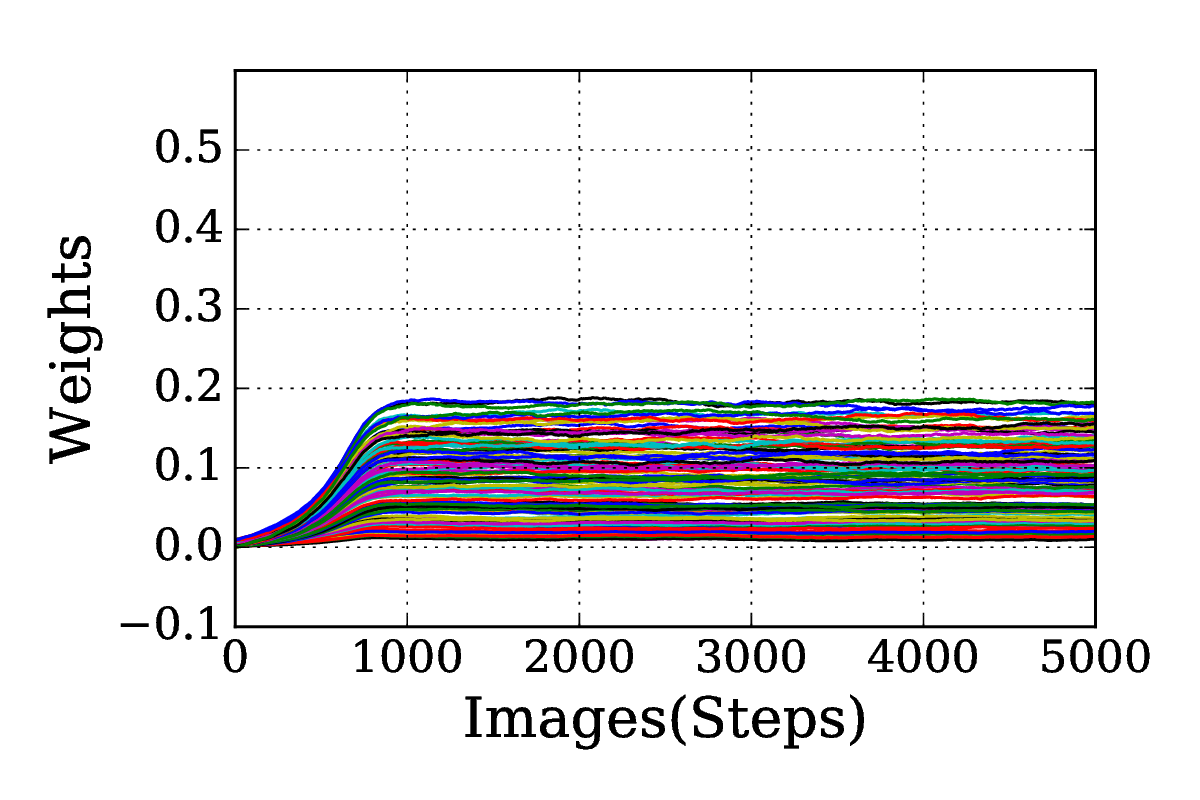
\includegraphics[width=\textwidth]{pics_sdlm/30_exp_RBM/exp2_weights_non.png}
		\caption{Weights of Exp2}
	\end{subfigure}
	\begin{subfigure}[t]{0.45\textwidth}
		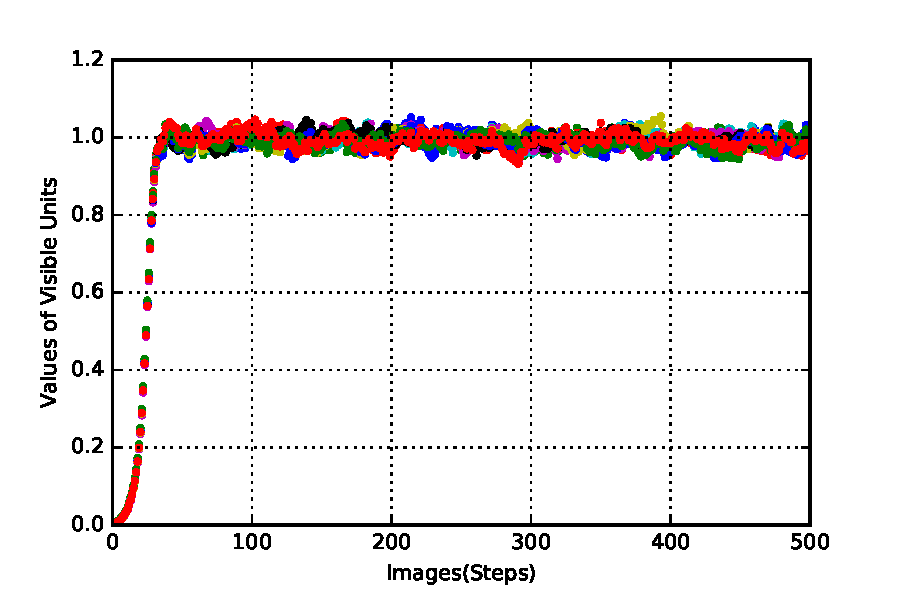
\includegraphics[width=\textwidth]{pics_sdlm/30_exp_RBM/exp1_recon_non.pdf}
		\caption{Reconstruction of visible units in Exp1}
	\end{subfigure}
	\begin{subfigure}[t]{0.45\textwidth}
		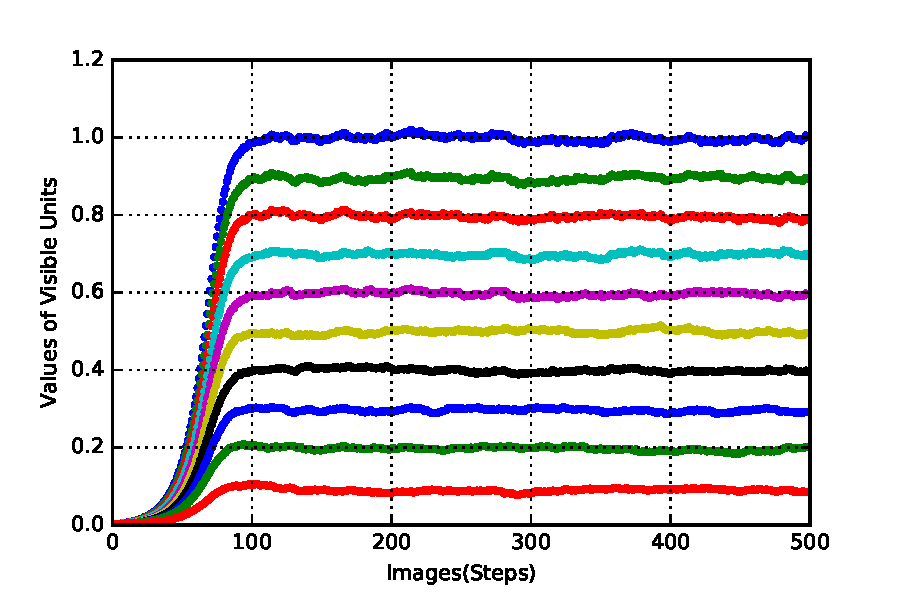
\includegraphics[width=\textwidth]{pics_sdlm/30_exp_RBM/exp2_recon_non.pdf}
		\caption{Reconstruction of visible units in Exp2}
	\end{subfigure}\\
	\begin{subfigure}[t]{0.45\textwidth}
		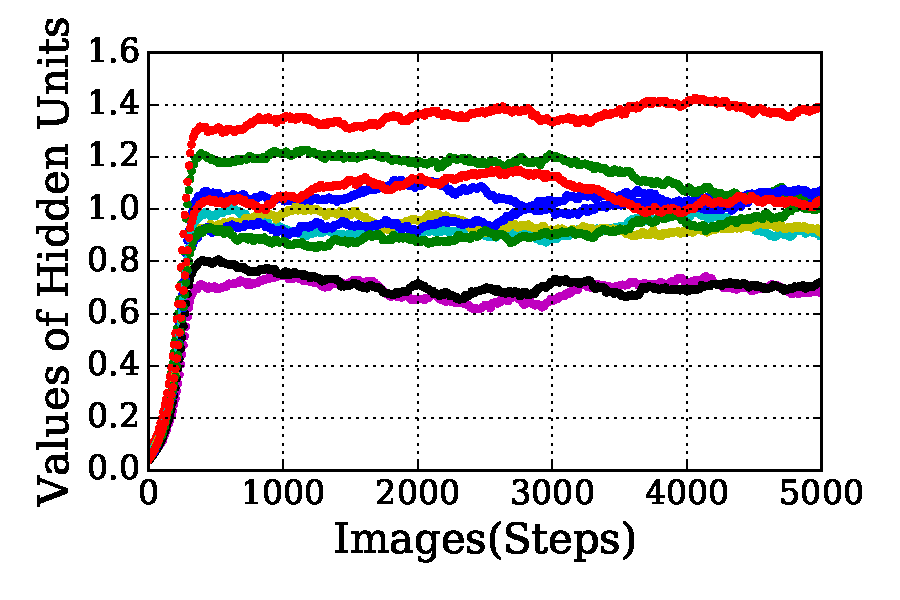
\includegraphics[width=\textwidth]{pics_sdlm/30_exp_RBM/exp1_hid_non.pdf}
		\caption{Output of hidden units in Exp1}
	\end{subfigure}
	\begin{subfigure}[t]{0.45\textwidth}
		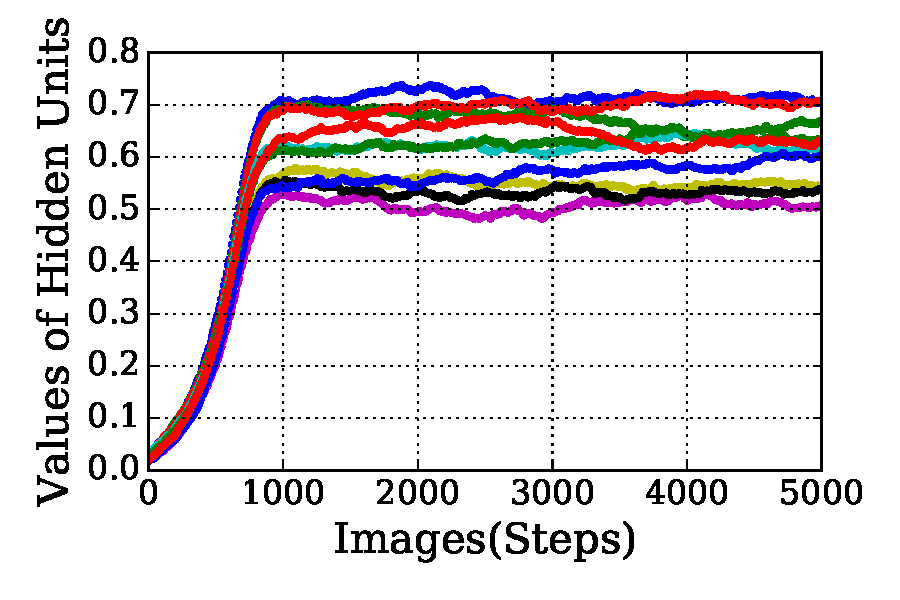
\includegraphics[width=\textwidth]{pics_sdlm/30_exp_RBM/exp2_hid_non.pdf}
		\caption{Output of hidden units in Exp2}
	\end{subfigure}\\
	\begin{subfigure}[t]{0.45\textwidth}
		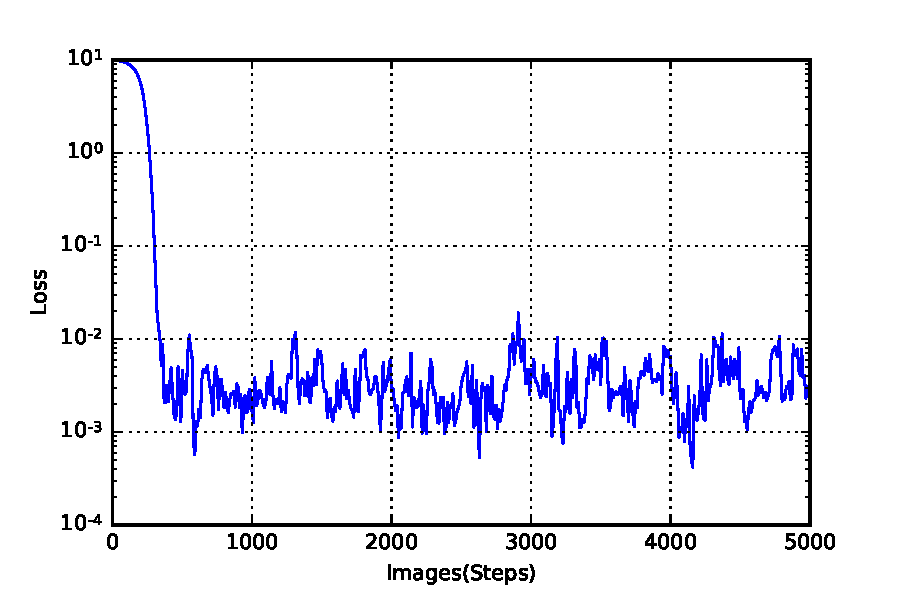
\includegraphics[width=\textwidth]{pics_sdlm/30_exp_RBM/exp1_loss.pdf}
		\caption{Output of hidden units in Exp1}
	\end{subfigure}
	\begin{subfigure}[t]{0.45\textwidth}
		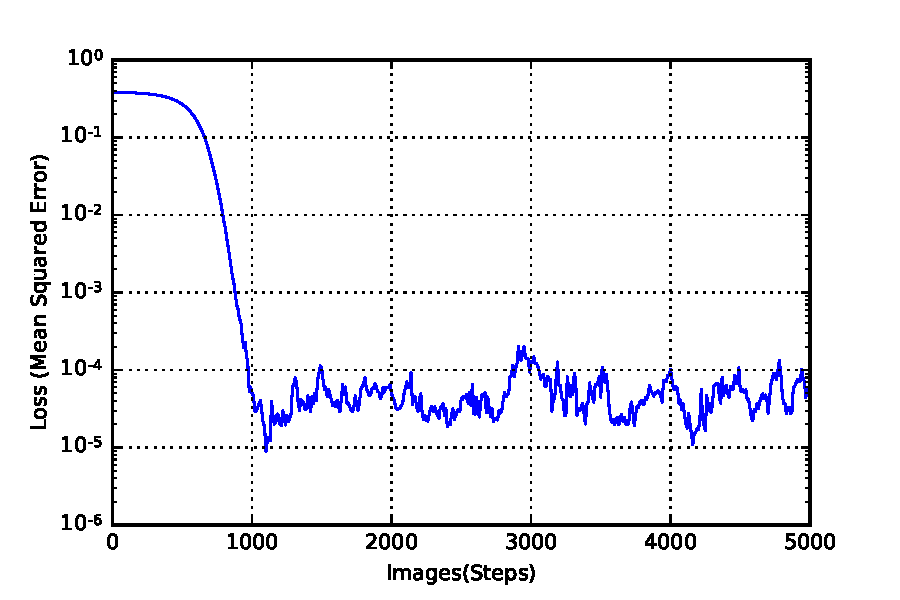
\includegraphics[width=\textwidth]{pics_sdlm/30_exp_RBM/exp2_loss.pdf}
		\caption{Output of hidden units in Exp2}
	\end{subfigure}
	\caption{Changes of weights, output of visible and hidden units, and mean squared error (loss) during the nRBM training of the reconstruction tests. 
		Experiments 1) 10 visible units fully connected to 10 hidden units with input data of all 1s; 2) \DIFaddbeginFL \DIFaddFL{the }\DIFaddendFL same network fed with 10 values \DIFdelbeginFL \DIFdelFL{distribute }\DIFdelendFL \DIFaddbeginFL \DIFaddFL{distributed }\DIFaddendFL linearly from 0.1 to 1.}
	\label{fig:rbm_orig}
\end{figure}

\begin{figure}
	\centering
	\begin{subfigure}[t]{0.45\textwidth}
		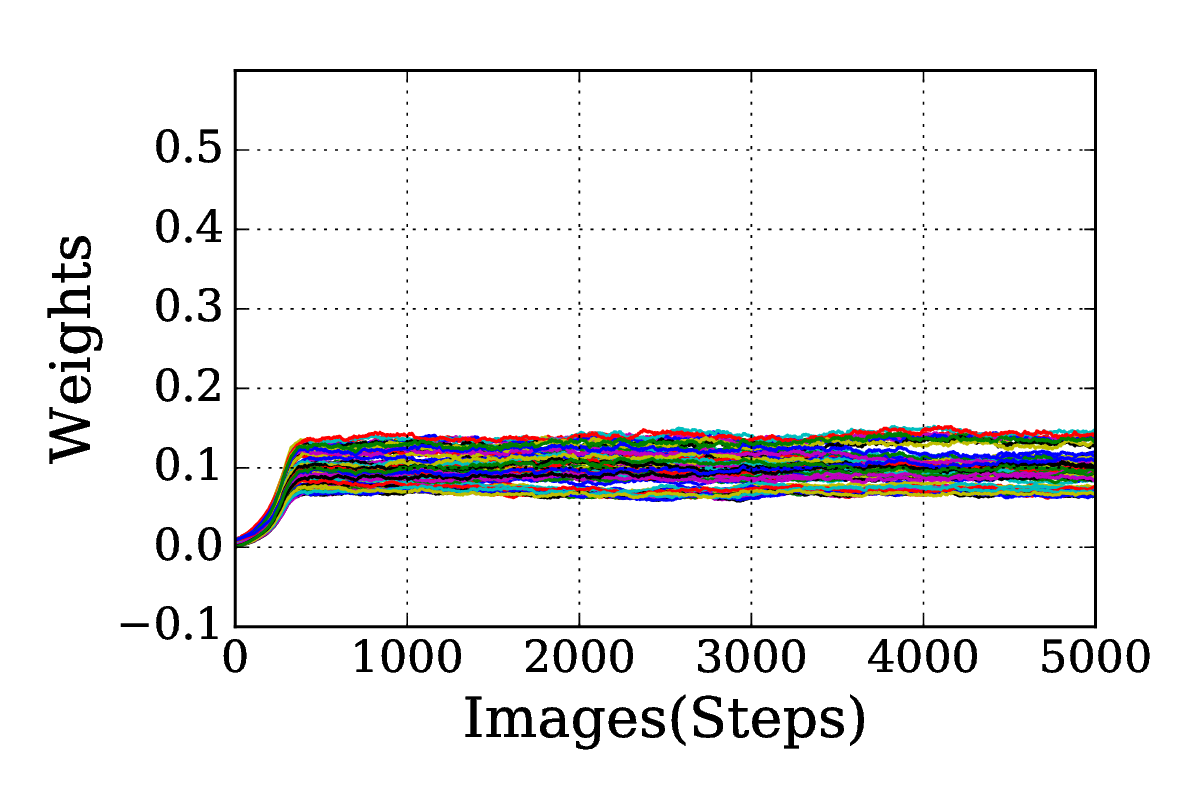
\includegraphics[width=\textwidth]{pics_sdlm/31_exp_RBM_noise/exp1_weights_s.png}
		\caption{Weights of Exp1}
	\end{subfigure}
	\begin{subfigure}[t]{0.45\textwidth}
		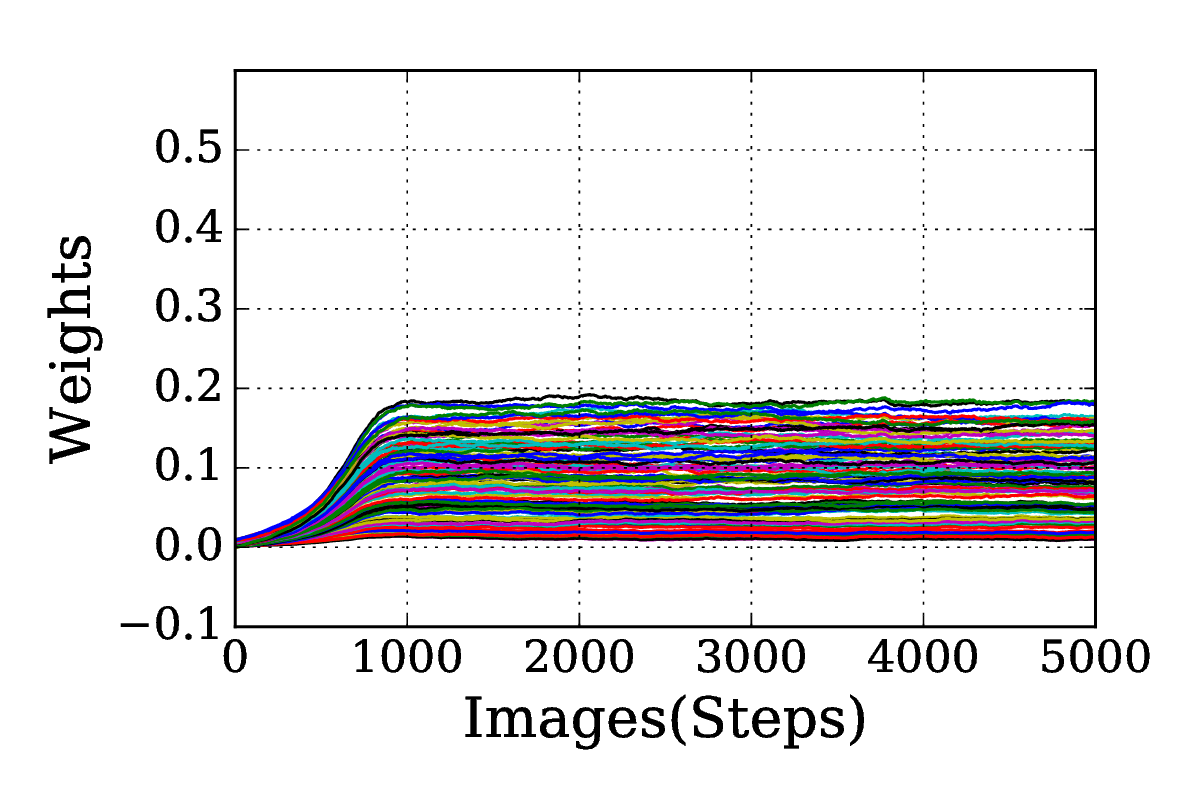
\includegraphics[width=\textwidth]{pics_sdlm/31_exp_RBM_noise/exp2_weights_s.png}
		\caption{Weights of Exp2}
	\end{subfigure}
	\begin{subfigure}[t]{0.45\textwidth}
		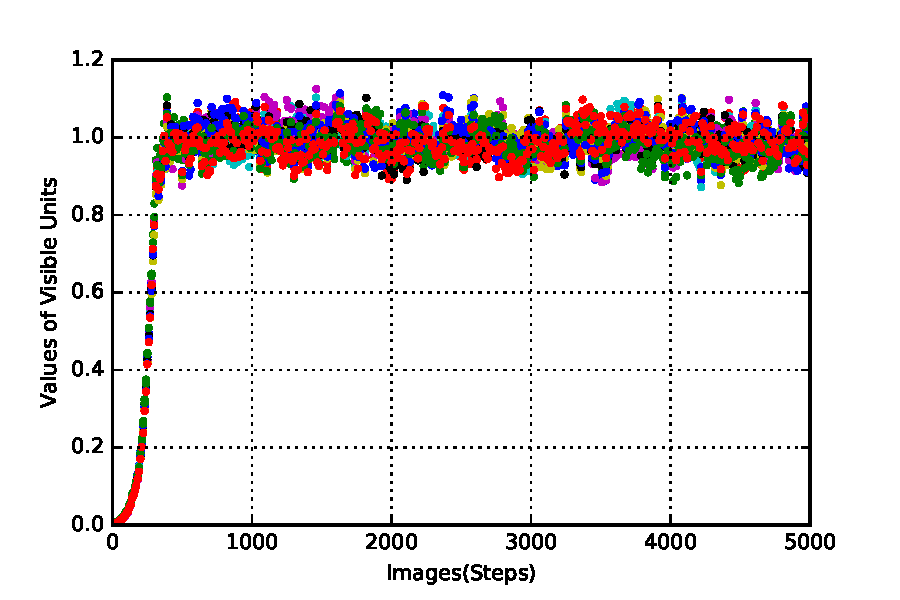
\includegraphics[width=\textwidth]{pics_sdlm/31_exp_RBM_noise/exp1_recon_s.pdf}
		\caption{Reconstruction of visible units in Exp1}
	\end{subfigure}
	\begin{subfigure}[t]{0.45\textwidth}
		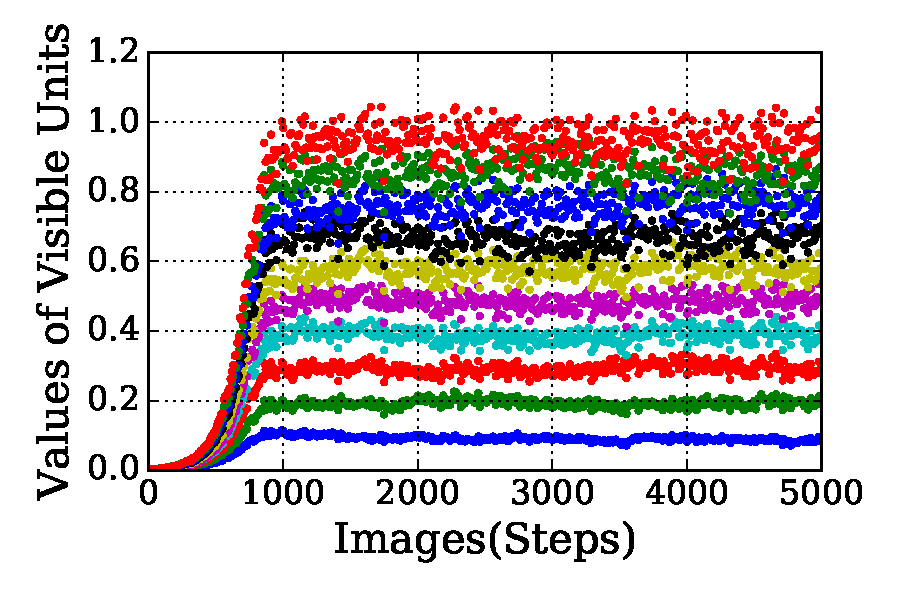
\includegraphics[width=\textwidth]{pics_sdlm/31_exp_RBM_noise/exp2_recon_s.pdf}
		\caption{Reconstruction of visible units in Exp2}
	\end{subfigure}\\
	\begin{subfigure}[t]{0.45\textwidth}
		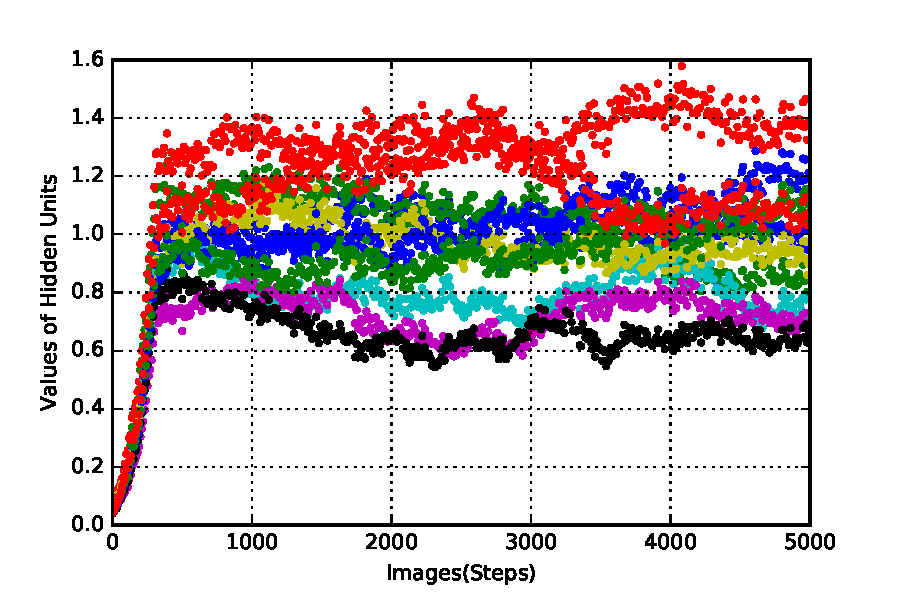
\includegraphics[width=\textwidth]{pics_sdlm/31_exp_RBM_noise/exp1_hid_s.pdf}
		\caption{Output of hidden units in Exp1}
	\end{subfigure}
	\begin{subfigure}[t]{0.45\textwidth}
		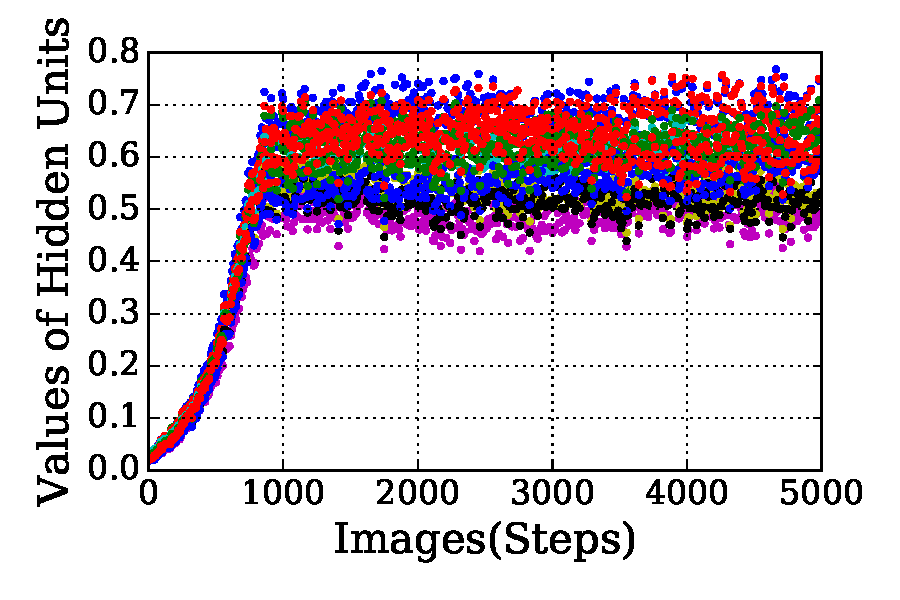
\includegraphics[width=\textwidth]{pics_sdlm/31_exp_RBM_noise/exp2_hid_s.pdf}
		\caption{Output of hidden units in Exp2}
	\end{subfigure}\\
	\begin{subfigure}[t]{0.45\textwidth}
		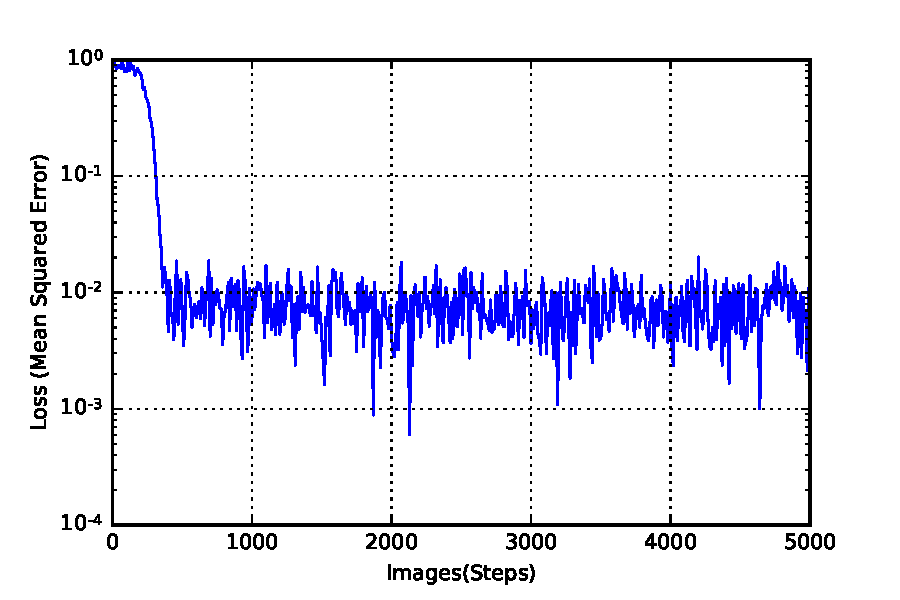
\includegraphics[width=\textwidth]{pics_sdlm/31_exp_RBM_noise/exp1_loss_s.pdf}
		\caption{Output of hidden units in Exp1}
	\end{subfigure}
	\begin{subfigure}[t]{0.45\textwidth}
		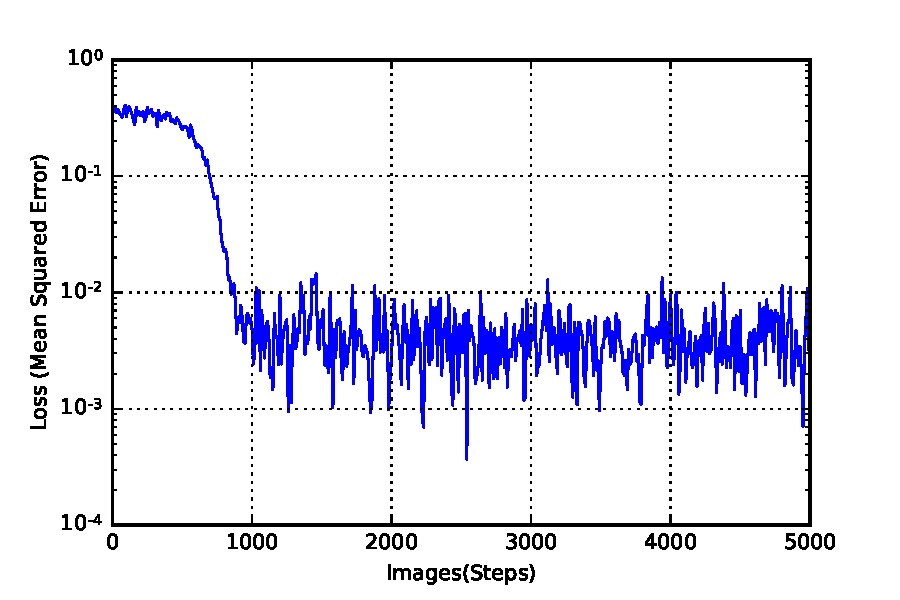
\includegraphics[width=\textwidth]{pics_sdlm/31_exp_RBM_noise/exp2_loss_s.pdf}
		\caption{Output of hidden units in Exp2}
	\end{subfigure}
	\caption{Changes of weights, output of visible and hidden units, and mean squared error (loss) during the nRBM training of the noisy reconstruction tests. 
		Experiments 1) 10 visible units fully connected to 10 hidden units with the count of Poisson spikes firing at 100~Hz which lasted 100~ms; 2) \DIFaddbeginFL \DIFaddFL{the }\DIFaddendFL same network fed with spike count of Poisson spikes at firing rate ranging from 10~Hz to 100~Hz.}
	\label{fig:rbm_noise}
\end{figure}

\subsection{Noisy Restricted Boltzmann Machines (nRBMs)}
Instead of using binary units and sigmoid activations \DIFdelbegin \DIFdel{in }\DIFdelend \DIFaddbegin \DIFadd{the }\DIFaddend RBM, we employed noisy ReLU (NReLU) units to construct \DIFaddbegin \DIFadd{an }\DIFaddend nRBM which was closer to biology and performed better in classification tasks~\citep{nair2010rectified}.
Leaving the learning algorithm unchanged, see Equation~\ref{equ:rbm_train} in Section~\ref{sec:rbm}:
\begin{equation}
\Delta w_{ij} = \eta (h_iv_j - h'_iv'_j),
\label{equ:rbm}
\end{equation} 
where \DIFaddbegin \DIFadd{a Gibbs sample comprises a pare of }\DIFaddend $h'_i$ and $v'_j$\DIFdelbegin \DIFdel{is a pair of Gibbs sampling}\DIFdelend , and the new sampling method NReLU is equivalent to generating multiple samples in the meantime and averaging them: $max(0, x+\mathcal{N}(0, \sigma(x))$.
The lower the variance of the normal distribution, the more samples are taken for averaging;
zero variance (equivalent to ReLU) is used when unlimited samples are generated, but at the same time the sampling itself loses the randomness.
In our experiments the variance of the normal distribution used in NReLU was 0.1 during training.
%While in testing, we used ReLU for the deterministic reconstructions. 
%To keep the similar network architecture and the learning rule with AEs, we used RBM with zero bias as well.
%Thus the weight updating rule in Equation~\ref{equ:rbm_train} can be described as:


Figure~\ref{fig:rbm_orig} demonstrates the training process and the \DIFdelbegin \DIFdel{testing result of }\DIFdelend \DIFaddbegin \DIFadd{test results of the }\DIFaddend nRBM; both experiments stabilised earlier than AE training: about 400 and $1,000$ steps respectively.
Due to \DIFaddbegin \DIFadd{the }\DIFaddend randomness of the sampling in \DIFaddbegin \DIFadd{the }\DIFaddend nRBM, there were noisy fluctuations adding on the weight change during training, the reconstructions and the output of hidden units in deterministic testing.
In addition, the loss stopped declining around $10^{-4}$ because of the same reason of randomness.

The same experiments were also carried out with the identical noisy input used in \DIFaddbegin \DIFadd{the }\DIFaddend SAE experiments, see Figure~\ref{fig:rbm_noise}.
The weight change was slightly noisier than the experiments on clean data, \DIFdelbegin \DIFdel{But }\DIFdelend \DIFaddbegin \DIFadd{but }\DIFaddend the noise was more obvious on the output of the visible reconstruction and the hidden units.
The same effect of the noisy input data can be found in Figure~\ref{fig:ae_noise} where the noise \DIFdelbegin \DIFdel{on }\DIFdelend \DIFaddbegin \DIFadd{in }\DIFaddend the reconstruction was much reduced compared to the input data and the loss remained about $10^{-2}$ and $10^{-2.5}$ after the stabilisation, although it took less time for \DIFaddbegin \DIFadd{the }\DIFaddend nRBM to converge than AE.


\subsection{Training Spiking Autoencoders (SAEs)}
\label{subsec:SAE}
Equation~\ref{equ:ae_widrow_hoff} states the learning rule of AE, which can be approximated by adding a positive SRM and a negative SRM in SNN training:
\begin{equation}
\label{equ:sae}
\begin{aligned}
\Delta w_{ij} &= \eta h_i v_j - \eta h_i v'_j \\
&= SRM(s_{h_i}, s_{v_j}) - SRM(s_{h_i}, s_{v'_j})~, \textrm{~where}\\
\eta_{s}&=\left \{
\begin{aligned}
 &\eta K^2 \tau\DIFdelbegin \DIFdel{_{dur} }\DIFdelend \DIFaddbegin \DIFadd{_{\textit{\textrm{dur}}} }\DIFaddend \tau\DIFdelbegin \DIFdel{_{win}}\DIFdelend \DIFaddbegin \DIFadd{_{\textit{\textrm{win}}}}\DIFaddend 10^{-6}~, ~\eta_{s+},~\textrm{~when weights potentiate,~and}\\
 & -\eta K^2 \tau\DIFdelbegin \DIFdel{_{dur} }\DIFdelend \DIFaddbegin \DIFadd{_{\textit{\textrm{dur}}} }\DIFaddend \tau\DIFdelbegin \DIFdel{_{win}}\DIFdelend \DIFaddbegin \DIFadd{_{\textit{\textrm{win}}}}\DIFaddend 10^{-6}~, ~\eta_{s-},~\textrm{~when weights depress.}
 \end{aligned} 
 \right.
\end{aligned} 
\end{equation}
We use simple linear Integrate-and-Fire (IF) neurons to validate the training algorithm, whose membrane potential follows the dynamics:
\begin{equation}
V_i(t+1)=V_i(t) + \sum_j w_{ij} s_j(t)~,
\end{equation}
and an IF neuron fires when \DIFaddbegin \DIFadd{the }\DIFaddend membrane potential $V$ surpasses the membrane threshold $V_{thresh}$, and $V$ resets to $V_{rest}$ after firing or when it reduces below \DIFdelbegin \DIFdel{than }\DIFdelend $V_{rest}$.
The parameters used are listed in \DIFdelbegin \DIFdel{the }\DIFdelend Table~\ref{tbl:srm}.
\begin{table}[th]
	\centering
	\caption{\label{tbl:srm}Parameter setting of SRM and IF neurons for training SAEs and SRBMs.}
	\bgroup
	\def\arraystretch{1.2}
	\begin{tabular}{c c l}
		%\hline
		Parameters & Values & Description \\
		\hline
		K & 100 & linear scaling factor\\
		%\hline
		\DIFdelbeginFL \DIFdelFL{$\tau_{dur}$ }\DIFdelendFL \DIFaddbeginFL \DIFaddFL{$\tau_{\textit{\textrm{dur}}}$ }\DIFaddendFL & 100 ms &  length of training spike trains\\
		%\hline
		\DIFdelbeginFL \DIFdelFL{$\tau_{win}$ }\DIFdelendFL \DIFaddbeginFL \DIFaddFL{$\tau_{\textit{\textrm{win}}}$ }\DIFaddendFL & 10 ms & window length of STDP\\
		%\hline
		$\eta$ & $10^{-3}$ & learning rate of AEs and RBMs\\
		%\hline
		$\eta_{s+}$ & $10^{-4}$ & positive learning rate of SAEs and SRBMs\\
		$\eta_{s-}$ & $-10^{-4}$ & negative learning rate of SAEs and SRBMs\\
		%\hline
		$V_{rest}$ & 0~mV & resting membrane potential\\
		%\hline
		$V_{thresh}$ & 1~mV & membrane threshold  \\
	\end{tabular}
	\egroup
\end{table}


The weight increase takes place in the positive STDP learning between the neurons of the input ($\bf{v}$) and the hidden units ($\bf{h}$); 
the weight decrease is carried out in the negative STDP learning between the reconstruction ($\bf{v'}$) and the hidden neurons ($\bf{h}$).
Figure~\ref{fig:sym_conn} shows the network architecture of an SAE where the hidden units connect to the reconstruction neurons with the weight matrix $\bf{w}$ and the input neurons feedforward to the hidden layer with the transposed tied weights $\bf{w}^\textrm{T}$.
The shared weights, \DIFaddbegin \DIFadd{with the }\DIFaddend three individual populations of neurons\DIFaddbegin \DIFadd{, }\DIFaddend compose the training network of an SAE.

\begin{figure}[th]
	\centering
	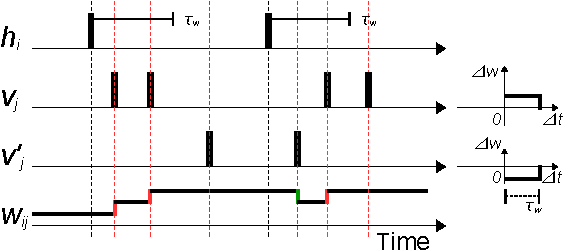
\includegraphics[width=0.7\textwidth]{pics_sdlm/rSTDP.pdf}
	\caption{How SRM works in training spiking Autoencoders.}
	\label{fig:rSTDP}
\end{figure}

\begin{figure}
	\centering
	\begin{subfigure}[t]{0.45\textwidth}
		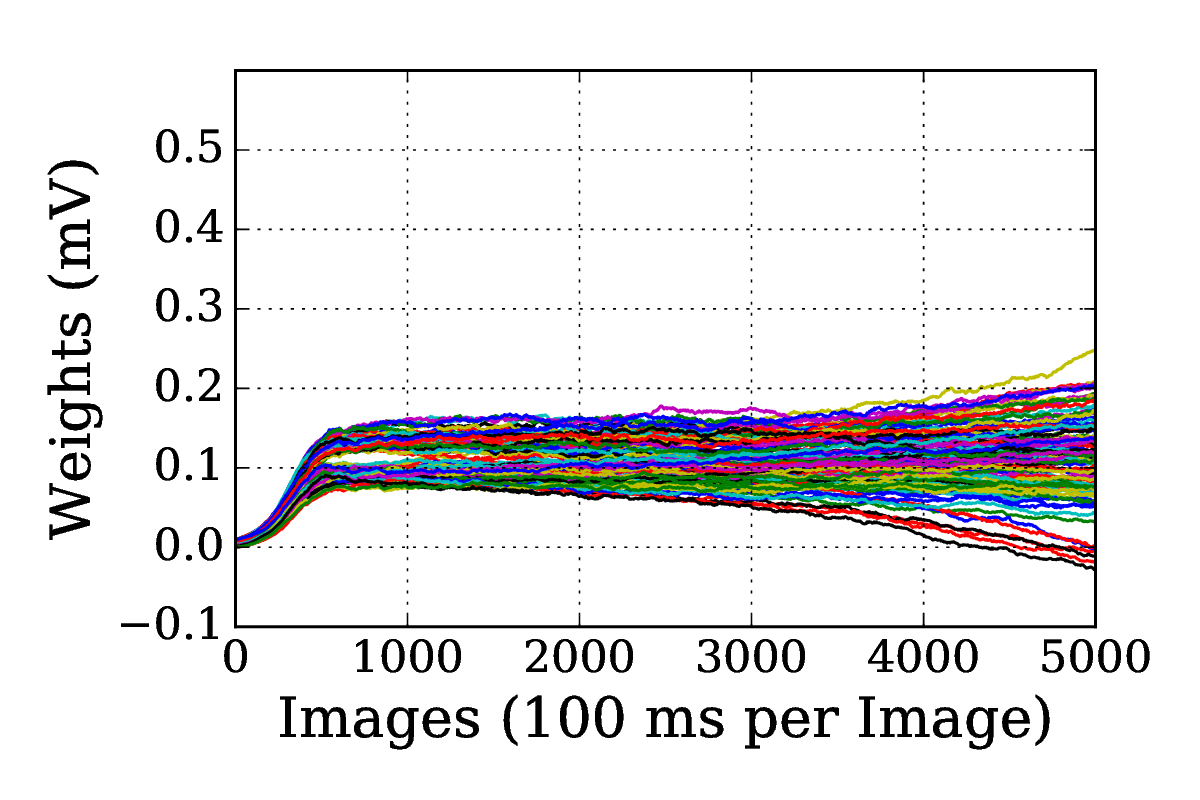
\includegraphics[width=\textwidth]{pics_sdlm/00_exp_SAE_Orig/exp1_weights_s.png}
		\caption{Weights of Exp1}
	\end{subfigure}
	\begin{subfigure}[t]{0.45\textwidth}
		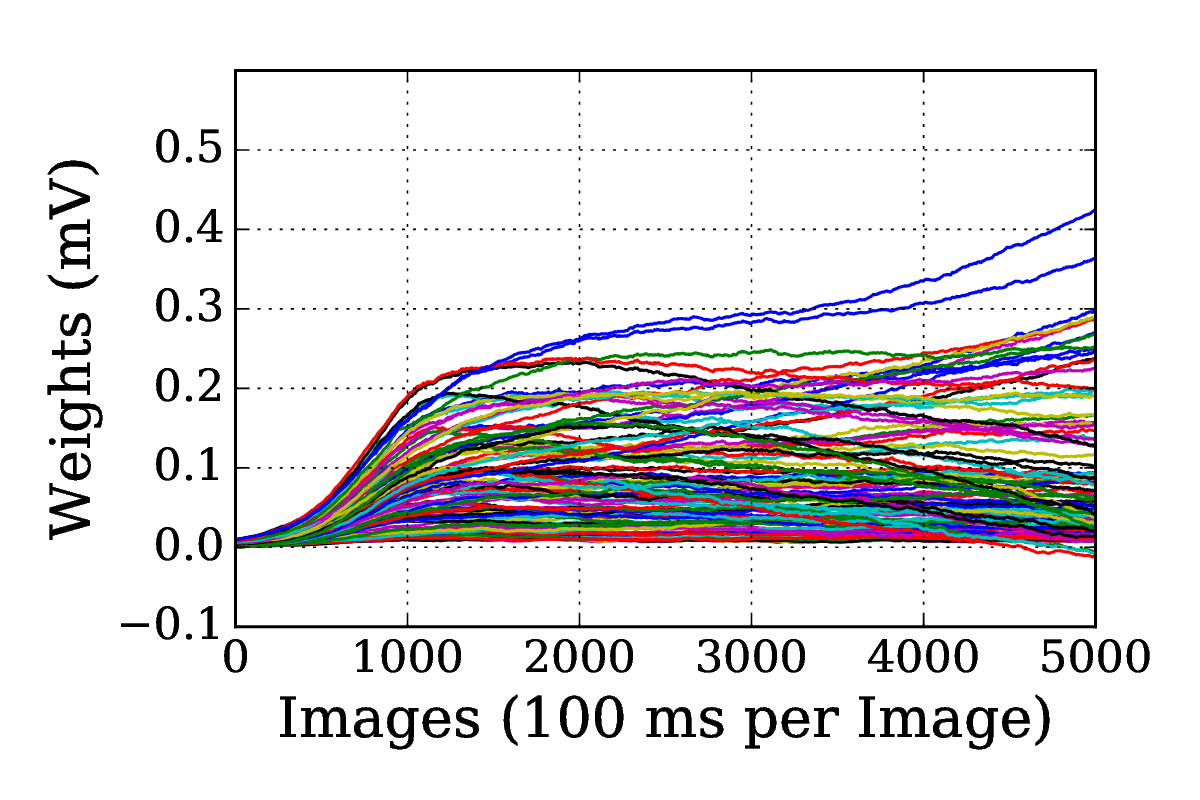
\includegraphics[width=\textwidth]{pics_sdlm/00_exp_SAE_Orig/exp2_weights_s.png}
		\caption{Weights of Exp2}
	\end{subfigure}
	\begin{subfigure}[t]{0.45\textwidth}
		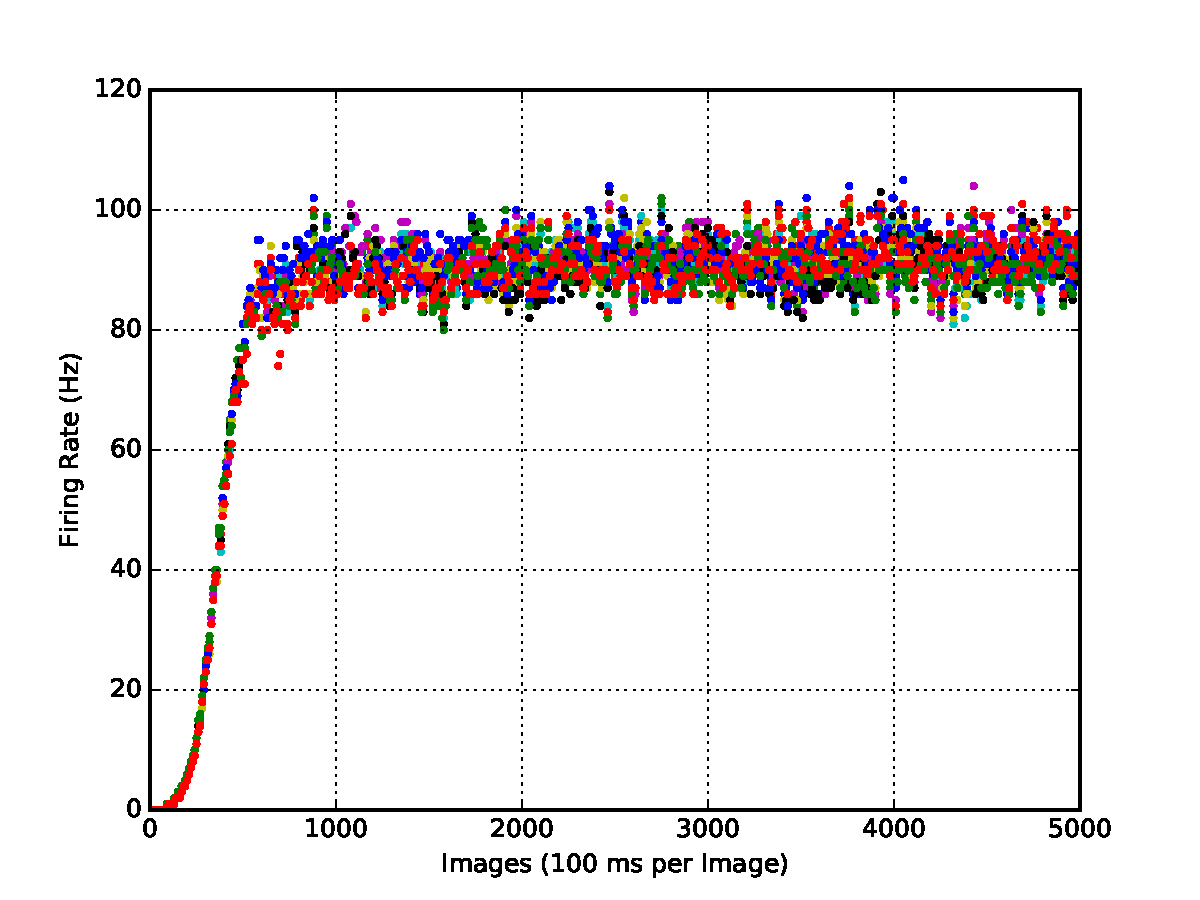
\includegraphics[width=\textwidth]{pics_sdlm/00_exp_SAE_Orig/exp1_recon_s.pdf}
		\caption{Reconstruction of visible units in Exp1}
	\end{subfigure}
	\begin{subfigure}[t]{0.45\textwidth}
		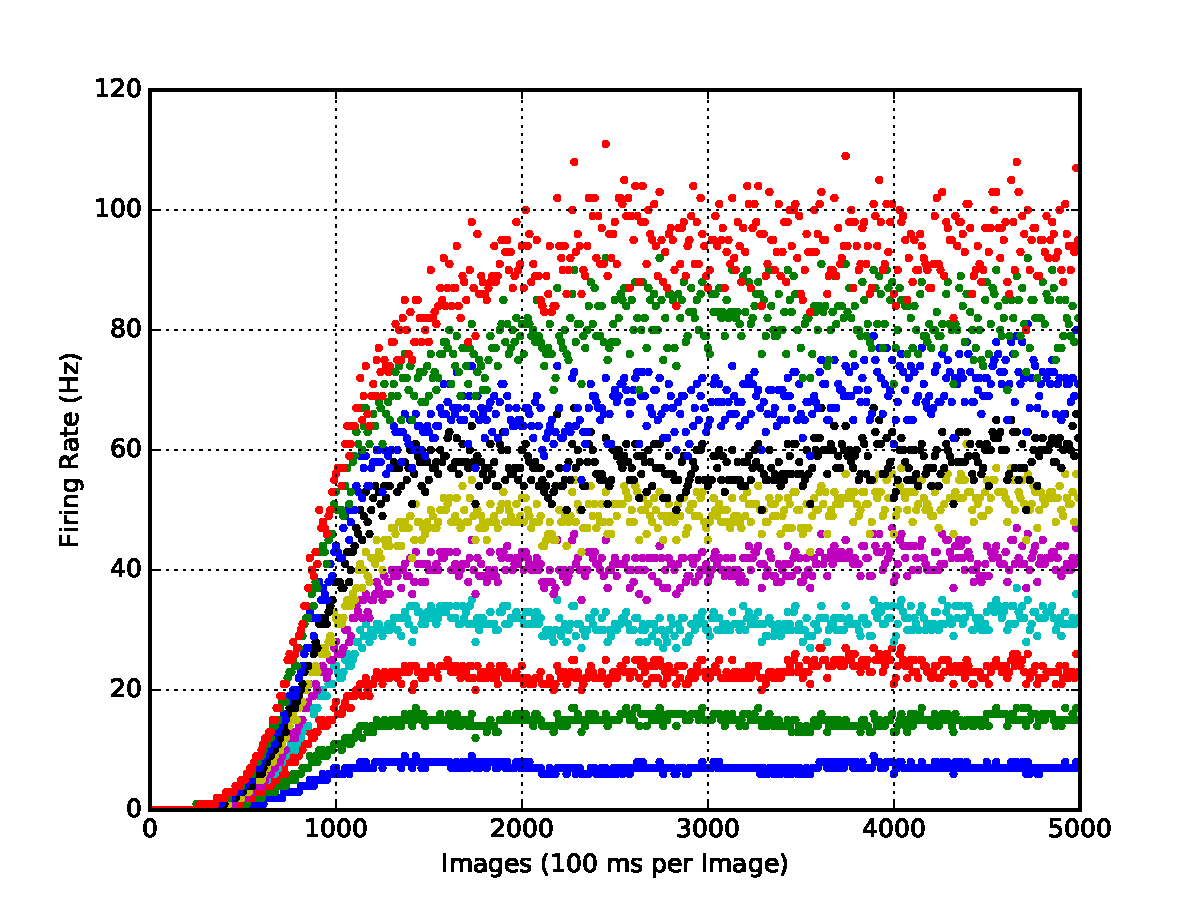
\includegraphics[width=\textwidth]{pics_sdlm/00_exp_SAE_Orig/exp2_recon_s.pdf}
		\caption{Reconstruction of visible units in Exp2}
	\end{subfigure}\\
	\begin{subfigure}[t]{0.45\textwidth}
		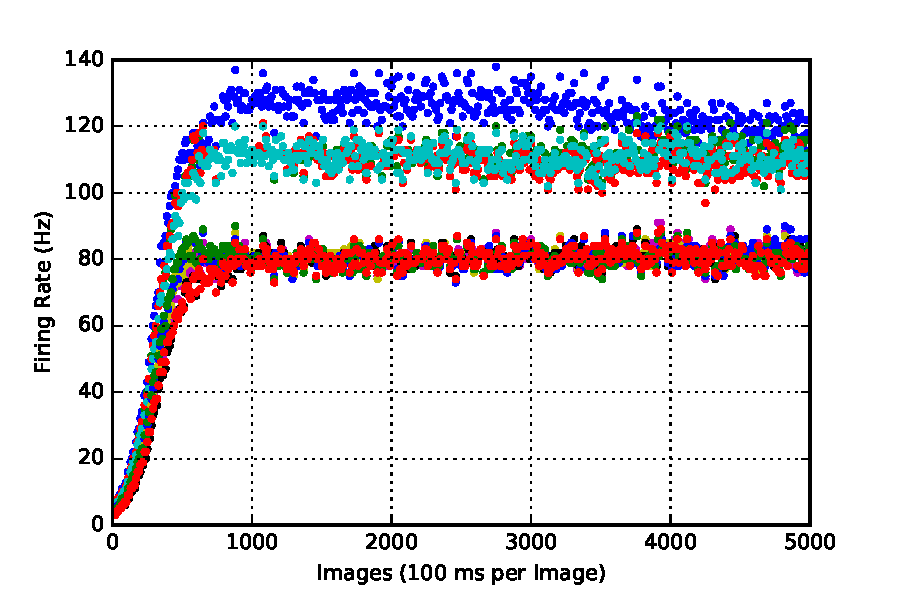
\includegraphics[width=\textwidth]{pics_sdlm/00_exp_SAE_Orig/exp1_hid_s.pdf}
		\caption{Output of hidden units in Exp1}
	\end{subfigure}
	\begin{subfigure}[t]{0.45\textwidth}
		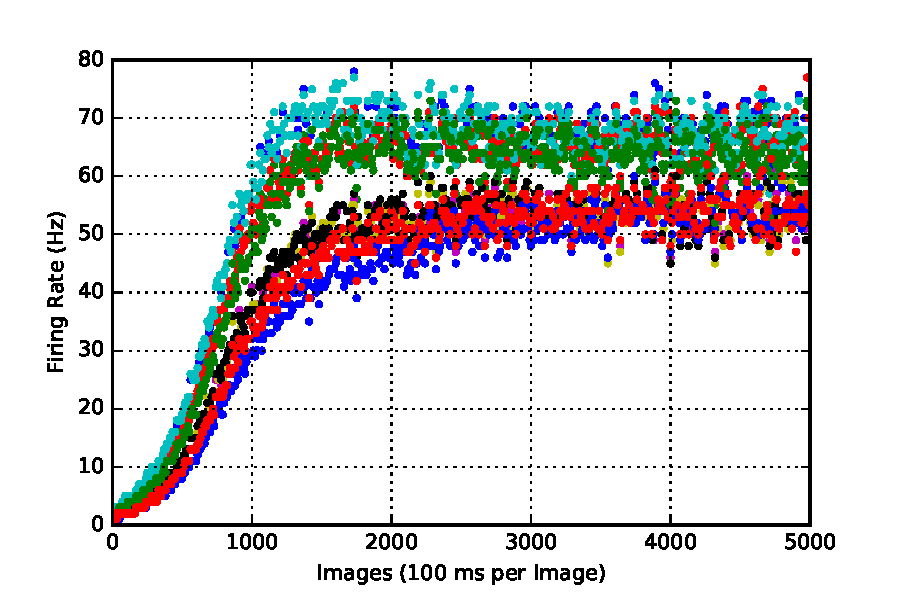
\includegraphics[width=\textwidth]{pics_sdlm/00_exp_SAE_Orig/exp2_hid_s.pdf}
		\caption{Output of hidden units in Exp2}
	\end{subfigure}\\
	\begin{subfigure}[t]{0.45\textwidth}
		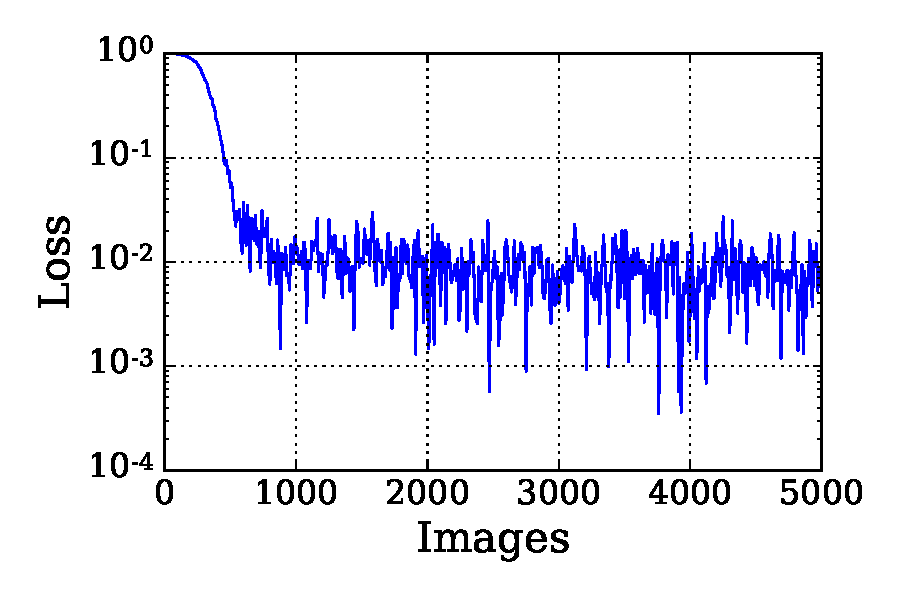
\includegraphics[width=\textwidth]{pics_sdlm/00_exp_SAE_Orig/exp1_mse_nons.pdf}
		\caption{Loss of Exp1}
	\end{subfigure}
	\begin{subfigure}[t]{0.45\textwidth}
		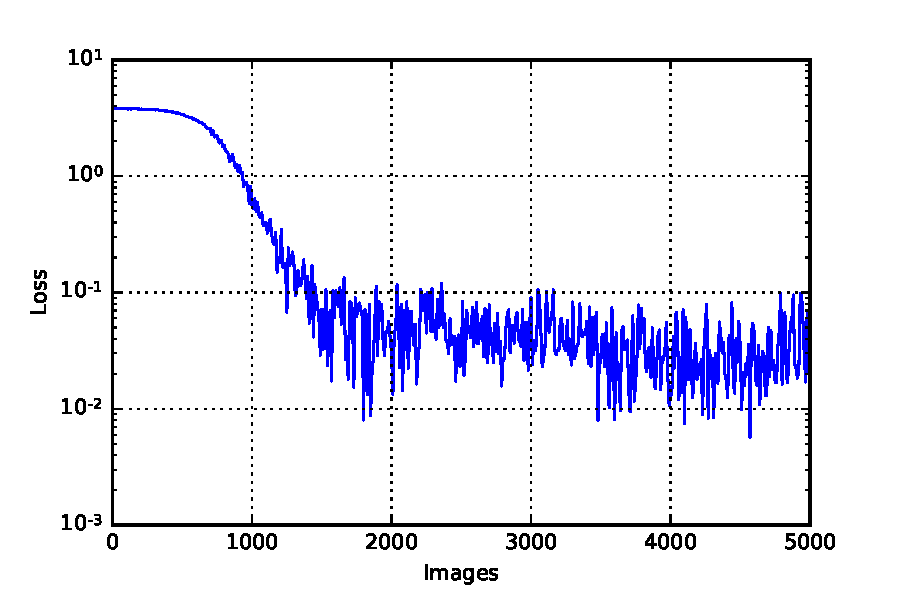
\includegraphics[width=\textwidth]{pics_sdlm/00_exp_SAE_Orig/exp2_mse_nons.pdf}
		\caption{Loss of Exp2}
	\end{subfigure}
	\caption{Weights and firing rates of visible and hidden units change during training of the reconstruction tests of spiking AE. 
		Experiments 1) 10 visible units fully connected to 10 hidden units with Poisson spike trains of 100~Hz which lasted 100~ms; 2) \DIFaddbeginFL \DIFaddFL{the }\DIFaddendFL same network fed with 10 Poisson spike trains of firing rate ranging from 10~Hz to 100~Hz.}
	\label{fig:SAE_orig}
\end{figure}

Figure~\ref{fig:rSTDP} illustrates the learning mechanism of the SAE architecture by giving an example of one hidden neuron $h_i$ connected \DIFdelbegin \DIFdel{by }\DIFdelend \DIFaddbegin \DIFadd{to }\DIFaddend an input neuron $v_j$ and connecting to a reconstruction neuron $v'_j$ with the same strength $w_{ij}$.
The weight $w_{ij}$ rises by $\eta_{s+}$ (marked with \DIFaddbegin \DIFadd{an }\DIFaddend up-arrow) when a spike comes within the period of \DIFdelbegin \DIFdel{$\tau_{win}$ }\DIFdelend \DIFaddbegin \DIFadd{$\tau_{\textit{\textrm{win}}}$ }\DIFaddend after the hidden neuron fires;
and it decreases by $\eta_{s-}$ (marked with \DIFaddbegin \DIFadd{a }\DIFaddend down-arrow) if the reconstruction neuron generates a spike in the same time window.
If either $v_j$ or $v'_j$ spikes outside the effective STDP window, the weight will remain unchanged.
The learning continues as long as the neurons are active, however the weights may stay relatively stable when the input firing rate is the same as the \DIFdelbegin \DIFdel{reconstructions'}\DIFdelend \DIFaddbegin \DIFadd{reconstruction's}\DIFaddend .

To reproduce the experiments of the AEs, we selected the parameters (see Table~\ref{tbl:srm}) for training SAEs and also apply the same parameters for SRBM experiments.
Each input vector (image) was presented as spiking trains with the length of 100~ms, and the STDP window was set to 10~ms.
The input values scaled up by $K=100$~Hz were used as firing rates of the spike trains.
Therefore, according to Equation~\ref{equ:eta_s}, the learning rate of SAEs and SRBMs was $\pm 10^{-4}$.

To compare with the AE experiments on noisy input data, Figure~\ref{fig:SAE_orig} records the weight change during training and the results generated by the testing on each image presented for 1~s.
The most important and obvious difference was the weight change where the weights did not stabilise but their values diverged during training.
%The output firing rate of the hidden units tends to converge as training procedes on.
The reason for the phenomena will be discussed in Section~\ref{sec:problem}.
The training was slower than the AE experiments and the loss took longer \DIFdelbegin \DIFdel{time }\DIFdelend to decrease to \DIFdelbegin \DIFdel{a }\DIFdelend \DIFaddbegin \DIFadd{the }\DIFaddend same level.
\DIFdelbegin \DIFdel{It }\DIFdelend \DIFaddbegin \DIFadd{This }\DIFaddend was mainly caused by the low firing rate of both input and hidden units at the beginning of the training.
Thus, few, even \DIFdelbegin \DIFdel{none}\DIFdelend \DIFaddbegin \DIFadd{no}\DIFaddend , spikes triggered STDP.
With the simple input of Exp1, the training performance reached the same level of 0.01 in loss comparing to the noisy AE test;
however, the SAE did not reconstruct the various input values of Exp2 as accurately as the AE did, since the parameters \DIFdelbegin \DIFdel{$\tau_{win}$ and $\tau_{dur}$ }\DIFdelend \DIFaddbegin \DIFadd{$\tau_{\textit{\textrm{win}}}$ and $\tau_{\textit{\textrm{dur}}}$ }\DIFaddend were relatively short.

\subsection{Training Spiking RBM}
\begin{figure}[h]
	\centering
		\begin{subfigure}[c]{0.33\textwidth}
			\includegraphics[width=\textwidth]{pics_sdlm/rbm.pdf}
		\end{subfigure}
		\begin{subfigure}[c]{0.66\textwidth}
			\includegraphics[width=\textwidth]{pics_sdlm/rSTDP_rbm.pdf}
		\end{subfigure}
	\caption{Network architecture and the learning algorithm of a spiking RBM.}
	\label{fig:sRBM}
\end{figure}

As illustrated in Equation~\ref{equ:rbm}, the positive weight change is generated from multiplication of visible and hidden units where the weight depression comes from the \DIFdelbegin \DIFdel{pair of Gibbs sampling}\DIFdelend \DIFaddbegin \DIFadd{product of the Gibbs sampled hidden and reconstruction values}\DIFaddend .
Figure~\ref{fig:sRBM} shows the architecture of an SRBM which consists of four layers of neurons: input $\bf{v}$, hidden $\bf{h}$, Gibbs visible (or reconstruction) $\bf{v'}$ and Gibss hidden $\bf{h'}$ neurons, and the shared weights $\bf{W}$.

Figure~\ref{fig:sRBM} demonstrates the training of an SRBM with a pair of spiking neurons $v_j$ and $h_i$, the corresponding Gibbs sampling pair $v'_j$ and $h'_i$, and the shared weight $w_{ij}$.
Up-arrows mark the increase of the weight when $v_j$ fires during the time window after the spikes of $h_i$;
meanwhile, \DIFdelbegin \DIFdel{down-arrow highlights }\DIFdelend \DIFaddbegin \DIFadd{down-arrows highlight	 }\DIFaddend the weight depression when $v'_j$ generates a spike no later than \DIFdelbegin \DIFdel{$\tau_{win}$ }\DIFdelend \DIFaddbegin \DIFadd{$\tau_{\textit{\textrm{win}}}$ }\DIFaddend after $h'_i$ fires.
%The amplitudes of the weight change, $\eta_{s+}$ and $\eta_{s-}$, were set the same as in Table~\ref{tbl:srm}.


%\begin{figure}
%	\centering
%	\includegraphics[width=0.7\textwidth]{pics_sdlm/rSTDP_rbm.pdf}
%	\caption{How SRM works in training spiking RBMs.}
%	\label{fig:rSTDP_rbm}
%\end{figure}



\begin{figure}
	\centering
	\begin{subfigure}[t]{0.45\textwidth}
		\includegraphics[width=\textwidth]{pics_sdlm/10_exp_SRBM_Orig/exp1_weights_s.png}
		\caption{Weights of Exp1}
	\end{subfigure}
	\begin{subfigure}[t]{0.45\textwidth}
		\includegraphics[width=\textwidth]{pics_sdlm/10_exp_SRBM_Orig/exp2_weights_s.png}
		\caption{Weights of Exp2}
	\end{subfigure}
	\begin{subfigure}[t]{0.45\textwidth}
		\includegraphics[width=\textwidth]{pics_sdlm/10_exp_SRBM_Orig/exp1_recon_s.pdf}
		\caption{Reconstruction of visible units in Exp1}
	\end{subfigure}
	\begin{subfigure}[t]{0.45\textwidth}
		\includegraphics[width=\textwidth]{pics_sdlm/10_exp_SRBM_Orig/exp2_recon_s.pdf}
		\caption{Reconstruction of visible units in Exp2}
	\end{subfigure}\\
	\begin{subfigure}[t]{0.45\textwidth}
		\includegraphics[width=\textwidth]{pics_sdlm/10_exp_SRBM_Orig/exp1_hid_s.pdf}
		\caption{Output of hidden units in Exp1}
	\end{subfigure}
	\begin{subfigure}[t]{0.45\textwidth}
		\includegraphics[width=\textwidth]{pics_sdlm/10_exp_SRBM_Orig/exp2_hid_s.pdf}
		\caption{Output of hidden units in Exp2}
	\end{subfigure}\\
	\begin{subfigure}[t]{0.45\textwidth}
		\includegraphics[width=\textwidth]{pics_sdlm/10_exp_SRBM_Orig/exp1_mse_nons.pdf}
		\caption{Loss of Exp1}
	\end{subfigure}
	\begin{subfigure}[t]{0.45\textwidth}
		\includegraphics[width=\textwidth]{pics_sdlm/10_exp_SRBM_Orig/exp2_mse_nons.pdf}
		\caption{Loss of Exp2}
	\end{subfigure}
	\caption{Weights and firing rates of visible and hidden units change during training of the reconstruction tests of \DIFaddbeginFL \DIFaddFL{a }\DIFaddendFL spiking RBM. 
		Experiments 1) 10 visible units fully connected to 10 hidden units with Poisson spike trains of 100~Hz which lasted 100~ms; 2) \DIFaddbeginFL \DIFaddFL{the }\DIFaddendFL same network fed with 10 Poisson spike trains of firing rate ranging from 10~Hz to 100~Hz.}
\label{fig:srbm_orig}
\end{figure}

The weight divergence was a more severe problem in \DIFaddbegin \DIFadd{the }\DIFaddend SRBM, see Figure~\ref{fig:srbm_orig}.
Especially for Exp1, only one hidden neuron was active on the later half of the training, thus \DIFdelbegin \DIFdel{to make }\DIFdelend \DIFaddbegin \DIFadd{making the }\DIFaddend firing rate of the reconstruction \DIFdelbegin \DIFdel{jumping }\DIFdelend \DIFaddbegin \DIFadd{jump }\DIFaddend between two states.
Because of the high firing rate of the pre-synaptic neuron, a slight weight increase may generate quite a few spikes for the post-synaptic neuron.
Therefore, more balanced activity among hidden neurons can perform better in terms of reconstruction accuracy.
%The same as SAE experiments, the slower training and worse loss also appear in the experiments.

\section{Problem of \DIFdelbegin \DIFdel{Spikes Correlation}\DIFdelend \DIFaddbegin \DIFadd{Spike Correlations	}\DIFaddend }
\label{sec:problem}
From the experiments above, the problem of non-convergence of weight searching appeared in training of SAEs and SRBMs using SRM.
Instead of stabilising at a (local) minima of the parameter space, the values of the weights continued to grow or to decay, in fact to diverge, even after the loss locked to a certain level.
The diverging weights not only made the loss increase, for example \DIFaddbegin \DIFadd{as }\DIFaddend shown in Figure~\ref{fig:srbm_orig}(g), but also led the weights too far from the expected effective range of the AE or RBM training.

The diverging weight values were caused by \DIFdelbegin \DIFdel{the }\DIFdelend correlations between spike trains.
Note that the rate multiplication of two spike trains (stated in Equation~\ref{equ:mul}) works under the condition of the independence between the spike trains.
However, the spike trains generated by a layer of neurons are strongly correlated to the spikes which the lower layer feeds them; and also influence the spike firing of the upper layer.
Therefore, any pair of spike trains $\bf{v}$ and $\bf{h}$, and $\bf{h}$ and $\bf{v'}$ in training SAEs are correlated, so are the spikes of $\bf{h'}$ and $\bf{v'}$ of SRBMs.


Taking SAE training for example, the strength of some synapses continuously increases because they have a relatively strong weight to trigger hidden units to fire, but the hidden unit taking their transposed weights have a weaker impact on the firing of the reconstruction neuron.
Thus the correlation between $v_j$ and $h_i$ is stronger than $v'_j$ and $h_i$, making the positive weight update more \DIFdelbegin \DIFdel{frequent }\DIFdelend \DIFaddbegin \DIFadd{frequently }\DIFaddend than it drops.
On the contrary, the decreasing weights appear in the opposite situation when $h_i$ correlates stronger with $v'_j$ than $v_j$.
Regarding \DIFdelbegin \DIFdel{to }\DIFdelend \DIFaddbegin \DIFadd{the }\DIFaddend SRBM, the training is even more effected by the correlations where the values of the weights diverge at a faster pace.

 
This section proposes three solutions to reduce the correlation between \DIFaddbegin \DIFadd{spike trains of different }\DIFaddend layers of neurons \DIFdelbegin \DIFdel{, with the purpose of training spiking deep learning models approximately to the process of their conventional training methods.
The aim is to modulate the weight updates close to }\DIFdelend \DIFaddbegin \DIFadd{thus approximating }\DIFaddend AE and RBM training \DIFdelbegin \DIFdel{under the premise of keeping a similar level of loss.
}\DIFdelend \DIFaddbegin \DIFadd{with equivalent event-based on-line learning of SAEs and SRBMs using SRM.
%DIF > training spiking Deep Learning models approximately to the process of their conventional training methods.
%DIF > The aim is to modulate the weight updates close to AE and RBM training under the premise of keeping a similar level of loss.
}\DIFaddend To highlight the performance of the solutions, we apply these methods \DIFdelbegin \DIFdel{on }\DIFdelend \DIFaddbegin \DIFadd{to }\DIFaddend the same experiments above\DIFdelbegin \DIFdel{.
And }\DIFdelend \DIFaddbegin \DIFadd{, and }\DIFaddend the default parameters are the same as in Table\ref{tbl:srm}.
\begin{figure}
	\centering
	\begin{subfigure}[c]{0.45\textwidth}\raggedleft
		\myrowlabel{Orignal SAE}
		\raisebox{-.5\height}{\includegraphics[width=.9\textwidth]
			{pics_sdlm/00_exp_SAE_Orig/exp2_weights_s.png}}\\
		\myrowlabel{S1}
		\raisebox{-.5\height}{\includegraphics[width=.9\textwidth]
			{pics_sdlm/01_exp_SAE_Orig_long/exp2_weights_s.png}}\\
		\myrowlabel{S2}
		\raisebox{-.5\height}{\includegraphics[width=.9\textwidth]
			{pics_sdlm/03_exp_SAE_noise_long/exp2_weights_s.png}}
		\myrowlabel{S3}
		\raisebox{-.5\height}{\includegraphics[width=.9\textwidth]
			{pics_sdlm/05_exp_SAE_teach_long/exp2_weights_s.png}}\\
		\myrowlabel{S4}
		\raisebox{-.5\height}{\includegraphics[width=.9\textwidth]
			{pics_sdlm/07_exp_SAE_all_long/exp2_weights_s.png}}
		\caption{Exp2 Weights}
	\end{subfigure}%
	\hspace{1em}
	\begin{subfigure}[c]{0.45\textwidth}\raggedleft
		\raisebox{-.5\height}{\includegraphics[width=.9\textwidth]
			{pics_sdlm/00_exp_SAE_Orig/exp2_mse_nons.pdf}}\\
		\raisebox{-.5\height}{\includegraphics[width=.9\textwidth]
			{pics_sdlm/01_exp_SAE_Orig_long/exp2_mse_nons.pdf}}\\
		\raisebox{-.5\height}{\includegraphics[width=.9\textwidth]
			{pics_sdlm/03_exp_SAE_noise_long/exp2_mse_nons.pdf}}
		\raisebox{-.5\height}{\includegraphics[width=.9\textwidth]
			{pics_sdlm/05_exp_SAE_teach_long/exp2_mse_nons.pdf}}\\
		\raisebox{-.5\height}{\includegraphics[width=.9\textwidth]
			{pics_sdlm/07_exp_SAE_all_long/exp2_mse_nons.pdf}}
		\caption{Exp2 Loss}
	\end{subfigure}%
	\caption{Comparisons of weights and loss of solutions for training SAE on Exp2: [S1] longer STDP window, [S2] noisy threshold, [S3] teaching signal, and [S4] combined solutions. 10 visible units fully \DIFdelbeginFL \DIFdelFL{connected }\DIFdelendFL \DIFaddbeginFL \DIFaddFL{connects }\DIFaddendFL to 10 hidden units with Poisson spike trains of firing rate ranging from 10~Hz to 100~Hz.}
	\label{fig:sols_ae}
\end{figure}

\begin{figure}
	\centering
	\begin{subfigure}[c]{0.45\textwidth}\raggedleft
		\myrowlabel{Orignal SRBM}
		\raisebox{-.5\height}{\includegraphics[width=.9\textwidth]
			{pics_sdlm/10_exp_SRBM_Orig/exp2_weights_s.png}}\\
		\myrowlabel{S1}
		\raisebox{-.5\height}{\includegraphics[width=.9\textwidth]
			{pics_sdlm/11_exp_SRBM_Orig_long/exp2_weights_s.png}}\\
		\myrowlabel{S2}
		\raisebox{-.5\height}{\includegraphics[width=.9\textwidth]
			{pics_sdlm/13_exp_SRBM_noise_long/exp2_weights_s.png}}
		\myrowlabel{S3}
		\raisebox{-.5\height}{\includegraphics[width=.9\textwidth]
				{pics_sdlm/15_exp_SRBM_teach_long/exp2_weights_s.png}}\\
		\myrowlabel{S4}
		\raisebox{-.5\height}{\includegraphics[width=.9\textwidth]
			{pics_sdlm/17_exp_SRBM_all_long/exp2_weights_s.png}}
		\caption{Exp2 Weights}
	\end{subfigure}%
	\hspace{1em}
	\begin{subfigure}[c]{0.45\textwidth}\raggedleft
		\raisebox{-.5\height}{\includegraphics[width=.9\textwidth]
			{pics_sdlm/10_exp_SRBM_Orig/exp2_mse_nons.pdf}}\\
		\raisebox{-.5\height}{\includegraphics[width=.9\textwidth]
			{pics_sdlm/11_exp_SRBM_Orig_long/exp2_mse_nons.pdf}}\\
		\raisebox{-.5\height}{\includegraphics[width=.9\textwidth]
			{pics_sdlm/13_exp_SRBM_noise_long/exp2_mse_nons.pdf}}
		\raisebox{-.5\height}{\includegraphics[width=.9\textwidth]
			{pics_sdlm/15_exp_SRBM_teach_long/exp2_mse_nons.pdf}}\\
		\raisebox{-.5\height}{\includegraphics[width=.9\textwidth]
			{pics_sdlm/17_exp_SRBM_all_long/exp2_mse_nons.pdf}}
		\caption{Exp2 Loss}
	\end{subfigure}%
	\caption{Comparisons of weights and loss of solutions for training SRBM on Exp2: [S1] longer STDP window, [S2] noisy threshold, [S3] teaching signal, and [S4] combined solutions. 10 visible units fully \DIFdelbeginFL \DIFdelFL{connected }\DIFdelendFL \DIFaddbeginFL \DIFaddFL{connects }\DIFaddendFL to 10 hidden units with Poisson spike trains of firing rate ranging from 10~Hz to 100~Hz.}
	\label{fig:sols_rbm}
\end{figure}

\subsection{Solution~1~(S1): Longer STDP Window}
A stronger weight between a pair of pre- and post-synaptic neurons \DIFdelbegin \DIFdel{makes }\DIFdelend \DIFaddbegin \DIFadd{results in }\DIFaddend a higher probability for the pre-synaptic neuron to trigger a post-synaptic spike in a shorter period; 
%v and h can be reversed in experiments! maybe show some result.
a weaker connection strength usually takes longer to activate a spike.
Thus SRM using a short STDP window produces a lower rate multiplication of a neuron pair with weaker synaptic strength.
Therefore, we use a longer square STDP window to accumulate more evidence \DIFdelbegin \DIFdel{making SRM less bias on }\DIFdelend \DIFaddbegin \DIFadd{to improve the accuracy of SRM of spike trains with low frequency and }\DIFaddend weak connections and \DIFdelbegin \DIFdel{more independent on }\DIFdelend \DIFaddbegin \DIFadd{make SRM more independent of }\DIFaddend the correlations between spike trains.
Of course, an unlimited window length is ideal to eliminate the effect of neural correlations, but a fair trade-off also takes computation and memory use into account.
In the experiment, we doubled the window length to 20~ms and set $\eta_s$ to $\pm 5 \times 10^{-5}$, and recorded the complete results in \DIFdelbegin \DIFdel{Figure}\DIFdelend \DIFaddbegin \DIFadd{Figures}\DIFaddend ~\ref{fig:sol1_ae} and~\ref{fig:sol1_rbm} in \DIFdelbegin \DIFdel{Appendices}\DIFdelend \DIFaddbegin \DIFadd{Appendix~\ref{sec:app2}}\DIFaddend .

To make the comparisons more straightforward, we list the weights and loss \DIFdelbegin \DIFdel{of }\DIFdelend \DIFaddbegin \DIFadd{recorded from }\DIFaddend Exp2\DIFaddbegin \DIFadd{, which is described in Section~\ref{sec:dSNN} where AEs and RBMs reconstruct 10 float numbers from 0.1 to 1.0, }\DIFaddend for all the solutions in Figure~\ref{fig:sols_ae} (SAE) and Figure~\ref{fig:sols_rbm} (SRBM).
\DIFdelbegin \DIFdel{A }\DIFdelend \DIFaddbegin \DIFadd{The }\DIFaddend longer STDP window reduced the weight divergence that the bidirectional weight change slowed down and kept within a smaller range.
In addition, the loss dropped to a lower level compared to the original SAE test because the longer STDP window \DIFdelbegin \DIFdel{$\tau_{win}$ also made }\DIFdelend \DIFaddbegin \DIFadd{$\tau_{\textit{\textrm{win}}}$ also made the }\DIFaddend SRM more accurate which reflected \DIFdelbegin \DIFdel{to }\DIFdelend the first property of \DIFaddbegin \DIFadd{the }\DIFaddend SRM algorithm in Section~\ref{sec:SRM}.



\subsection{Solution~2~(S2): Noisy Threshold}
%There are various ways to introduce noise in formal spiking neuron models~\citep{gerstner2014neuronal}.
We introduce a method of `noisy threshold' (also called escape or hazard model)~\citep{gerstner2002spiking} to generate noise in the output of spikes.
The stochastic threshold of the membrane potential drives the post-synaptic spikes firing in advance or behind the expected time, thus reducing the correlation between the pre- and post synaptic spikes.
The Gaussian noise \DIFdelbegin \DIFdel{adding }\DIFdelend \DIFaddbegin \DIFadd{added }\DIFaddend to the membrane potential is randomly generated by $\mathcal{N}(0, \sigma)$~mV, where $\sigma$ is set to 0.2, 20\% of $V_{thresh} - V_{rest}.$
An appropriate $\sigma$ is chosen for introducing enough noise to decrease the correlation of the spike trains and also maintain a good loss performance.
The complete \DIFdelbegin \DIFdel{testing }\DIFdelend \DIFaddbegin \DIFadd{test }\DIFaddend results can be found in \DIFdelbegin \DIFdel{Appendices}\DIFdelend \DIFaddbegin \DIFadd{Appendix~\ref{sec:app2}}\DIFaddend , see Figures~\ref{fig:sol2_ae} and~\ref{fig:sol2_rbm}.

Using the same STDP window \DIFdelbegin \DIFdel{$\tau_{win}$ }\DIFdelend \DIFaddbegin \DIFadd{$\tau_{\textit{\textrm{win}}}$ }\DIFaddend of 20~ms, the noisy membrane threshold enhanced the decorrelation, thus the weight change remained more subtle than S1, see Figures~\ref{fig:sols_ae}(a) and~\ref{fig:sols_rbm}(a) .
Furthermore, the performance of the reconstruction improved in both SAE and SRBM training so that the loss reduced to a lower level and the training accelerated to reach stabilisation. % with the help of the noise. 


\subsection{Solution~3~(S3): Teaching Signal}
A \DIFdelbegin \DIFdel{teaching signal which fires }\DIFdelend \DIFaddbegin \DIFadd{Poisson spike train firing }\DIFaddend at the same rate as the input spikes \DIFdelbegin \DIFdel{is completely independent of }\DIFdelend \DIFaddbegin \DIFadd{but generated with a different random seed is independent of the equivalent input spike train and }\DIFaddend all the spikes generated in the network.
\DIFaddbegin \DIFadd{We call these spike trains teaching signals $\bf{s}$, because they are only used for weight updates but not conducted into the network.
}\DIFaddend Thus it decorrelates the \DIFaddbegin \DIFadd{spike trains used for }\DIFaddend SRM in the positive part of the weight change $\Delta w_{ij} = SRM(v_j,h_i)$ in SAE and SRBM by using $\Delta w_{ij}=SRM(s_j,h_i)$ instead, where $s_j$ is the teaching spike train firing at the same rate of $v_j$.
Compared to the other solutions, it requires doubled Poisson spike trains: the input spikes work the same to activate the network, and the teaching spikes do not impact on the neural dynamics but only trigger learning on the synapses between the input layer and the hidden layer.

In terms of SAE training, teaching signals alleviated the problem of correlations, as for the noisy threshold, and the variance of the loss shrinks (Figure~\ref{fig:sols_ae}[S3]).
Although the loss was kept at a higher level, it was due to a constant bias of the reconstruction which was caused by the stronger correlation on the negative SRM.
The reconstruction bias can be observed in the firing rates of the reconstruction neurons recorded in the complete experimental result in Figures~\ref{fig:sol2_ae} and~\ref{fig:sol2_rbm} \DIFdelbegin \DIFdel{of Appendices}\DIFdelend \DIFaddbegin \DIFadd{in Appendix~\ref{sec:app2}}\DIFaddend .
Regarding the SRBM training (Figure~\ref{fig:sols_rbm}), the weight divergence was also improved compared to S1 but not as good as S2, since the noisy threshold applied to the entire network whereas the teaching signal worked only on the input layer.
The average reconstruction loss was also worse than S1 and S2 because of the bias. 

\subsection{Test on Combined Solutions~(S4)}
The test combines solutions of long STDP window, noisy threshold and teaching signals.
The results shown in both Figures~\ref{fig:sols_ae} and~\ref{fig:sols_rbm} demonstrated a combined effect of the solutions, in that the dynamic trained weights were between the diverging degree of S2 and S3, and the loss level was kept in between.
More detailed experiments results can be found in Figures~\ref{fig:sol4_ae} and~\ref{fig:sol4_rbm} of Appendices.
%TODO add LIF tests
All of the above experiments and solutions were also tested on Leaky Integrate-and-Fire~(LIF) neurons to \DIFdelbegin \DIFdel{validates }\DIFdelend \DIFaddbegin \DIFadd{validate }\DIFaddend the features of \DIFaddbegin \DIFadd{the }\DIFaddend SRM that the accuracy was independent of neural models, see Figures~\ref{fig:LIF_sae} and~\ref{fig:LIF_srbm} in \DIFdelbegin \DIFdel{Appendices}\DIFdelend \DIFaddbegin \DIFadd{Appendix~\ref{sec:app2}}\DIFaddend .
The LIF neuron model follows the dynamics of its membrane potential, which decreases by a constant, $l=0.01$~mV, every time step :
\begin{equation}
V_i(t+1)=V_i(t) + \sum_j w_{ij} s_j(t) - l~.
\end{equation}
%XOR problem:
%To validate the decorrelation methods proposed, a more complicated reconstruction experiment is conducted.
%The input nodes are fed with values (x, y, z) sequentially (0, 0, 0), (0, 1, 1), (1, 0, 1) and (1, 1, 0) which follows XOR rules, z = x XOR y.
%9 visible units presented values of (x, y, z) by group of 3 and were fed with values of (0, 0, 0), (0, 1, 1), (1, 0, 1), (1, 1, 0) repeatedly with 100~ms Poisson spike trains firing at 100~Hz for 1, 0~Hz otherwise. And the visible units were fully connected to 9 hidden units.
%\begin{figure}
%	\centering
%	\begin{subfigure}[t]{0.32\textwidth}
%		\includegraphics[width=\textwidth]{pics_sdlm/21_exp_AE_noise/exp3_weights_s.png}
%		\caption{Weights of AE}
%	\end{subfigure}
%	\begin{subfigure}[t]{0.32\textwidth}
%		\includegraphics[width=\textwidth]{pics_sdlm/00_exp_SAE_Orig/exp3_weights_s.png}
%		\caption{Weights of Original SAE}
%	\end{subfigure}
%	\begin{subfigure}[t]{0.32\textwidth}
%		\includegraphics[width=\textwidth]{pics_sdlm/07_exp_SAE_all_long/exp3_weights_s.png}
%		\caption{Weights of Optimised SAE}
%	\end{subfigure}\\
%	\begin{subfigure}[t]{0.32\textwidth}
%		\includegraphics[width=\textwidth]{pics_sdlm/21_exp_AE_noise/exp3_recon_s2.pdf}
%		\caption{Reconstruction of visible units in AE}
%	\end{subfigure}
%	\begin{subfigure}[t]{0.32\textwidth}
%		\includegraphics[width=\textwidth]{pics_sdlm/00_exp_SAE_Orig/exp3_recon_s_2.pdf}
%		\caption{Reconstruction of visible units in Original SAE}
%	\end{subfigure}
%	\begin{subfigure}[t]{0.32\textwidth}
%		\includegraphics[width=\textwidth]{pics_sdlm/07_exp_SAE_all_long/exp3_recon_s_2.pdf}
%		\caption{Reconstruction of visible units in Optimised SAE}
%	\end{subfigure}\\
%	\begin{subfigure}[t]{0.32\textwidth}
%		\includegraphics[width=\textwidth]{pics_sdlm/21_exp_AE_noise/exp3_hid_s_2.pdf}
%		\caption{Output of hidden units in AE}
%	\end{subfigure}
%	\begin{subfigure}[t]{0.32\textwidth}
%		\includegraphics[width=\textwidth]{pics_sdlm/00_exp_SAE_Orig/exp3_hid_s_2.pdf}
%		\caption{Output of hidden units in Original SAE}
%	\end{subfigure}
%	\begin{subfigure}[t]{0.32\textwidth}
%		\includegraphics[width=\textwidth]{pics_sdlm/07_exp_SAE_all_long/exp3_hid_s_2.pdf}
%		\caption{Output of hidden units in Optimised SAE}
%	\end{subfigure}\\
%	\begin{subfigure}[t]{0.32\textwidth}
%		\includegraphics[width=\textwidth]{pics_sdlm/21_exp_AE_noise/exp3_loss_s_2.pdf}
%		\caption{Loss of AE}
%	\end{subfigure}
%	\begin{subfigure}[t]{0.32\textwidth}
%		\includegraphics[width=\textwidth]{pics_sdlm/00_exp_SAE_Orig/exp3_mse_nons_2.pdf}
%		\caption{Loss of Original SAE}
%	\end{subfigure}
%	\begin{subfigure}[t]{0.32\textwidth}
%		\includegraphics[width=\textwidth]{pics_sdlm/07_exp_SAE_all_long/exp3_mse_nons_2.pdf}
%		\caption{Loss of Optimised SAE}
%	\end{subfigure}
%	\caption{Experiment 3) Weights and firing rates of visible and hidden units change during training of the reconstruction tests of AE and spiking AE.}
%\end{figure}
%
%\begin{figure}
%	\centering
%	\begin{subfigure}[t]{0.32\textwidth}
%		\includegraphics[width=\textwidth]{pics_sdlm/31_exp_RBM_noise/exp3_weights_s.png}
%		\caption{Weights of RBM}
%	\end{subfigure}
%	\begin{subfigure}[t]{0.32\textwidth}
%		\includegraphics[width=\textwidth]{pics_sdlm/10_exp_SRBM_Orig/exp3_weights_s.png}
%		\caption{Weights of Original SRBM}
%	\end{subfigure}
%	\begin{subfigure}[t]{0.32\textwidth}
%		\includegraphics[width=\textwidth]{pics_sdlm/17_exp_SRBM_all_long/exp3_weights_s.png}
%		\caption{Weights of Optimised SRBM}
%	\end{subfigure}\\
%	\begin{subfigure}[t]{0.32\textwidth}
%		\includegraphics[width=\textwidth]{pics_sdlm/31_exp_RBM_noise/exp3_recon_s2.pdf}
%		\caption{Reconstruction of visible units in RBM}
%	\end{subfigure}
%	\begin{subfigure}[t]{0.32\textwidth}
%		\includegraphics[width=\textwidth]{pics_sdlm/10_exp_SRBM_Orig/exp3_recon_s_2.pdf}
%		\caption{Reconstruction of visible units in Original SRBM}
%	\end{subfigure}
%	\begin{subfigure}[t]{0.32\textwidth}
%		\includegraphics[width=\textwidth]{pics_sdlm/17_exp_SRBM_all_long/exp3_recon_s_2.pdf}
%		\caption{Reconstruction of visible units in Optimised SRBM}
%	\end{subfigure}\\
%	\begin{subfigure}[t]{0.32\textwidth}
%		\includegraphics[width=\textwidth]{pics_sdlm/31_exp_RBM_noise/exp3_hid_s_2.pdf}
%		\caption{Output of hidden units in RBM}
%	\end{subfigure}
%	\begin{subfigure}[t]{0.32\textwidth}
%		\includegraphics[width=\textwidth]{pics_sdlm/10_exp_SRBM_Orig/exp3_hid_s_2.pdf}
%		\caption{Output of hidden units in Original SRBM}
%	\end{subfigure}
%	\begin{subfigure}[t]{0.32\textwidth}
%		\includegraphics[width=\textwidth]{pics_sdlm/17_exp_SRBM_all_long/exp3_hid_s_2.pdf}
%		\caption{Output of hidden units in Optimised SRBM}
%	\end{subfigure}\\
%	\begin{subfigure}[t]{0.32\textwidth}
%		\includegraphics[width=\textwidth]{pics_sdlm/31_exp_RBM_noise/exp3_loss_s_2.pdf}
%		\caption{Loss of Optimised RBM}
%	\end{subfigure}
%	\begin{subfigure}[t]{0.32\textwidth}
%		\includegraphics[width=\textwidth]{pics_sdlm/10_exp_SRBM_Orig/exp3_mse_nons_2.pdf}
%		\caption{Loss of Original SRBM}
%	\end{subfigure}
%	\begin{subfigure}[t]{0.32\textwidth}
%		\includegraphics[width=\textwidth]{pics_sdlm/17_exp_SRBM_all_long/exp3_mse_nons_2.pdf}
%		\caption{Loss of Optimised SRBM}
%	\end{subfigure}
%	\caption{Experiment 3) Weights and firing rates of visible and hidden units change during training of the reconstruction tests of RBM and spiking SRBM.}
%\end{figure}


\section{Results: MNIST Test}
\DIFaddbegin \label{sec:SRM_result}
\DIFaddend Having discussed the problem of training \DIFdelbegin \DIFdel{of }\DIFdelend SAEs and SRBMs, we finally applied the proposed methods to \DIFaddbegin \DIFadd{the MNIST }\DIFaddend image recognition tasks\DIFdelbegin \DIFdel{of MNIST}\DIFdelend ;
the network architecture \DIFdelbegin \DIFdel{was }\DIFdelend \DIFaddbegin \DIFadd{is }\DIFaddend shown in Figure~\ref{fig:MNSIT}.
The training was conducted using a one-layer AE or RBM, which consisted of 794 visible units including 784 neurons representing the images, 10 label units marking the classification, and 500 neurons \DIFdelbegin \DIFdel{for }\DIFdelend \DIFaddbegin \DIFadd{are in }\DIFaddend the hidden layer.
During testing, only the 784 neurons representing image pixels remained as visible units and the other 10 label units worked as the top layer of an MLP network for recognising digits.
The trained weights of the one-layer AE/RBM were split into the bidirectional weights between visible and hidden units, and the forward connections from the hidden layer to the top layer.
The forward path of the network \DIFdelbegin \DIFdel{recognised }\DIFdelend \DIFaddbegin \DIFadd{assigned }\DIFaddend an image to a digit class, and the bidirectional connections reconstructed the input image.

\begin{figure}
	\centering
	\includegraphics[width=0.5\textwidth]{pics_sdlm/mnist.pdf}
	\caption{AE and RBM structure for MNIST tasks.}
	\label{fig:MNSIT}
\end{figure}

As the baseline for comparison, the same neural network architecture was firstly tested on conventional AE and nRBM, and then trained on SNNs.
Three epochs of all the $60,000$ training images were fed into the network in order.
In the training of SNNs, as described above in Section~\ref{sec:ae}, pixel values of images were represented by Poisson spike trains firing at a certain frequency linearly proportional to the original value.
The overall count of spikes for each pixel was used as a noisy input of conventional training, AE-NI and nRBM-NI, to provide an equal comparison to SNNs.
Moreover, all the training images were presented in sequence one by one in an on-line fashion, in other words we used the minimum batch size of~1.
%Since training a batch of $n$ images in parallel require $n$ times of physical spiking neurons sharing the same weights, it is easier to track the weight change caused by single pair of neurons than by $n$ pairs.
In addition, the default parameters of SNNs were the same as listed in Table~\ref{tbl:srm} except that in the improved solutions of SNN training the STDP window $tau_{win}$ was doubled to 20~ms and the learning rate $\eta_s$ was set to $5 \times 10^{-5}$ accordingly;
the initial weights were identical for all the experiments following as well as the input spike trains.


\subsection{Trained weights}

\begin{figure}
	\centering
	\begin{subfigure}[t]{0.4\textwidth}
		\includegraphics[width=\textwidth]{pics_sdlm/22_MNIST_AE/2_60000_0.pdf}
		\caption{AE}
	\end{subfigure}
	\begin{subfigure}[t]{0.4\textwidth}
		\includegraphics[width=\textwidth]{pics_sdlm/23_MNIST_AE_noise/2_60000_0.pdf}
		\caption{AE-NI}
	\end{subfigure}\\
	\begin{subfigure}[t]{0.4\textwidth}
		\includegraphics[width=\textwidth]{pics_sdlm/40_MNIST_SAE_original/2_60000_0.pdf}
		\caption{Original SAE}
	\end{subfigure}
	\begin{subfigure}[t]{0.4\textwidth}
		\includegraphics[width=\textwidth]{pics_sdlm/42_MNIST_SAE_noise/2_60000_0.pdf}
		\caption{SAE-S2}

	\end{subfigure}\\
	\begin{subfigure}[t]{0.4\textwidth}
		\includegraphics[width=\textwidth]{pics_sdlm/41_MNIST_SAE_teach/2_60000_0.pdf}
		\caption{SAE-S3}
	\end{subfigure}
	\begin{subfigure}[t]{0.4\textwidth}
		\includegraphics[width=\textwidth]{pics_sdlm/43_MNIST_SAE_all/2_60000_0.pdf}
		\caption{SAE-S4}
	\end{subfigure}\\
	\caption{Trained weights after 3 epochs of MNIST training using (a) AE, (b) AE-NI, Poisson spike trains as input data, (c) Original SAE, (d) SAE-S2, neurons \DIFdelbeginFL \DIFdelFL{of }\DIFdelendFL \DIFaddbeginFL \DIFaddFL{with }\DIFaddendFL noisy \DIFdelbeginFL \DIFdelFL{threshold}\DIFdelendFL \DIFaddbeginFL \DIFaddFL{thresholds}\DIFaddendFL , (e) SAE-S3, extra teaching signal, and (f) SAE-S4, combined solutions of S2 and S3.}
	\label{fig:weights_ae}
\end{figure}

\begin{figure}
	\centering
	\begin{subfigure}[t]{0.4\textwidth}
		\includegraphics[width=\textwidth]{pics_sdlm/32_MNIST_RBM/2_60000_0.pdf}
		\caption{nRBM}
	\end{subfigure}
	\begin{subfigure}[t]{0.4\textwidth}
		\includegraphics[width=\textwidth]{pics_sdlm/33_MNIST_RBM_noise/2_60000_0.pdf}
		\caption{nRBM-NI}
	\end{subfigure}\\
	\begin{subfigure}[t]{0.4\textwidth}
		\includegraphics[width=\textwidth]{pics_sdlm/50_MNIST_SRBM_original/2_60000_0.pdf}
		\caption{Original SRBM}
	\end{subfigure}
	\begin{subfigure}[t]{0.4\textwidth}
		\includegraphics[width=\textwidth]{pics_sdlm/52_MNIST_SRBM_noise/2_60000_0.pdf}
		\caption{SRBM-S2}
	\end{subfigure}	\\
	\begin{subfigure}[t]{0.4\textwidth}
		\includegraphics[width=\textwidth]{pics_sdlm/51_MNIST_SRBM_teach/2_60000_0.pdf}
		\caption{SRBM-S3}
	\end{subfigure}
	\begin{subfigure}[t]{0.4\textwidth}
		\includegraphics[width=\textwidth]{pics_sdlm/53_MNIST_SRBM_all/2_60000_0.pdf}
		\caption{SRBM-S4}
	\end{subfigure}\\
	\caption{Trained weights after 3 epochs of MNIST training using (a) nRBM, (b) nRBM-NI, Poisson spike trains as input data, (c) Original SRBM, (d) SRBM-S2, neurons \DIFdelbeginFL \DIFdelFL{of }\DIFdelendFL \DIFaddbeginFL \DIFaddFL{with }\DIFaddendFL noisy \DIFdelbeginFL \DIFdelFL{threshold}\DIFdelendFL \DIFaddbeginFL \DIFaddFL{thresholds}\DIFaddendFL , (e) SRBM-S3, extra teaching signal, and (f) SRBM-S4, combined solutions of S2 and S3.}
	\label{fig:weights_rbm}
\end{figure}

The first comparison was conducted directly on the trained weights after three epochs of the entire training images.
We randomly selected 49 hidden neurons out of 500 to display the weighs between the hidden and visible units (only the 784 neurons representing the images), see Figures~\ref{fig:weights_ae} and~\ref{fig:weights_rbm} where the grey scales from white to black represented the values between -0.1 to 0.1.
Unlike the diverging weights in the previous section, the trained weights of all the methods kept within a similar range thanks to the large dataset which restricted the weight searching to a certain scope.  



The trained weights of AE and AE-NI \DIFdelbegin \DIFdel{were of litter }\DIFdelend \DIFaddbegin \DIFadd{had little }\DIFaddend difference.
However, the original SAE training resulted in noisy trained patterns where unexpected white dots appeared on the extracted digit features (Figure~\ref{fig:weights_ae}(c)).
Nevertheless, the other improved SAE trainings demonstrated a closer feature extraction to the conventional \DIFdelbegin \DIFdel{AE's}\DIFdelend \DIFaddbegin \DIFadd{AEs}\DIFaddend .



Regarding RBM training
%, the extracted features were not easily recognisable as in the AE because of the randomness introduced by the noisy sampling of NReLU.
the results in Figure~\ref{fig:weights_rbm} \DIFdelbegin \DIFdel{shows}\DIFdelend \DIFaddbegin \DIFadd{show}\DIFaddend :
extracted features of \DIFdelbegin \DIFdel{nRBM were }\DIFdelend \DIFaddbegin \DIFadd{the nRBM }\DIFaddend consisted of continuous strokes although \DIFdelbegin \DIFdel{were not }\DIFdelend \DIFaddbegin \DIFadd{they were not as }\DIFaddend recognisable as those of \DIFaddbegin \DIFadd{the }\DIFaddend AE, due to the randomness introduced by the noisy sampling of NReLU;
\DIFdelbegin \DIFdel{noise of }\DIFdelend \DIFaddbegin \DIFadd{the noise in }\DIFaddend the input data led to the noisy extracted features where discontinuity of strokes appeared;
%are continuous and (b) pixel-wise noise appear in (b) of Poisson input in training conventional RBM;
few continuous strokes were generated in the original SRBM training;
but more noticeable extracted patterns turned up with the \DIFdelbegin \DIFdel{solution of noisy threshold }\DIFdelend \DIFaddbegin \DIFadd{noisy threshold solution }\DIFaddend of SRBM-S2;
patterns generated by SRBM-S3 training showed similar continuous strokes as in the original nRBM training;
and combined solutions demonstrated mixed patterns of training with S2 and S3 which was closer to the patterns trained with nRBM-NI. 


\subsection{Classification Accuracy (CA)}
As the most important metric to evaluate the training performance, we tested the classification accuracy on SNNs to compare with conventional models.
%Every image is presented as a vector of Poisson spike trains which last 1~ms long.
%All the experiments below are tested with the spike trains and the spike counts are used for the conventional AE and RBM testing of noisy input.
%On every millisecond step, we count the summed spikes of each output neuron since the start of the testing image's presentation.
The classification neuron having \DIFdelbegin \DIFdel{a }\DIFdelend \DIFaddbegin \DIFadd{the }\DIFaddend highest spike count indicated the predicted class of the given image.
%A correct recognition only happens when the prediction was the same as the label and only one prediction exists.
%Thus if two output neurons generate the same number of spikes which is the maximum, then the recognition is failed.

\begin{figure}
	\centering
	\begin{subfigure}[t]{0.8\textwidth}
		\includegraphics[width=\textwidth]{pics_sdlm/43_MNIST_SAE_all/compare_result.pdf}
		\caption{AEs and SAEs.}
%		\caption{Classification accuracy compared on AE and SAEs.}
	\end{subfigure}\\
	\begin{subfigure}[t]{0.8\textwidth}
		\includegraphics[width=\textwidth]{pics_sdlm/53_MNIST_SRBM_all/compare_result.pdf}
		\caption{nRBMs and SRBMs.}
%		\caption{Classification accuracy compared on RBM and SRBMs.}
	\end{subfigure}
	\caption{Classification accuracy \DIFdelbeginFL \DIFdelFL{compared }\DIFdelendFL \DIFaddbeginFL \DIFaddFL{comparing conventional models }\DIFaddendFL with \DIFdelbeginFL \DIFdelFL{traditional training method and }\DIFdelendFL spike-based models. All the \DIFdelbeginFL \DIFdelFL{trainings }\DIFdelendFL \DIFaddbeginFL \DIFaddFL{training }\DIFaddendFL started with same \DIFaddbeginFL \DIFaddFL{initial }\DIFaddendFL weights\DIFdelbeginFL \DIFdelFL{initialisation}\DIFdelendFL . Every 3K steps of training, the trained weights were recorded and tested on \DIFaddbeginFL \DIFaddFL{the }\DIFaddendFL MNIST testing dataset for classification accuracy. The Poisson spikes trains used for SNN simulations are identical for all the tests.}
	\label{fig:sdlm_ca}
\end{figure}
Shown in Figure~\ref{fig:sdlm_ca}(a), the CA of AE and AE-NI steadily increased until it reaches about 92\% with \DIFaddbegin \DIFadd{the }\DIFaddend first 20K images trained in the network.
The noise in the training images of AE-NI made the peak performance of 93.29\%, a bit lower than AE (93.76\%).
\DIFdelbegin \DIFdel{While the }\DIFdelend \DIFaddbegin \DIFadd{The }\DIFaddend training on SAEs was slower than \DIFaddbegin \DIFadd{on }\DIFaddend AE at the beginning, due to the reason (explained in Section~\ref{subsec:SAE}) of low spiking rates.
The classification performance of SAEs reached the AEs' \DIFaddbegin \DIFadd{after }\DIFaddend about 50K training steps, and started to diverge:
the original SAE kept a \DIFdelbegin \DIFdel{close CA of AE's }\DIFdelend \DIFaddbegin \DIFadd{CA close to that of AEs }\DIFaddend until it reached the best performance of 92.71\% at 87K steps, and then the CA began to decay because of the correlation problem;
while both SAE-S2 and SAE-S3 had similar performance \DIFdelbegin \DIFdel{with AEs and achieved }\DIFdelend \DIFaddbegin \DIFadd{to AEs and }\DIFaddend even overtook the best CA of AEs at 93.75\% and 94.38\% respectively;
and the combined solution SAE-S4 performed the best among all the models and achieved 94.72\% CA at 171K steps.

The nRBM was more sensitive to the noise of the training images than AE so that the CA of nRBM-NI slowly dropped and oscillated more and more strongly as training proceeded, see Figure~\ref{fig:sdlm_ca}(b).
The peak performances of nRBM and nRBM-NI appeared on 146K and 97K steps at 94.85\% and 93.16\% respectively. 
The quantitative testing results of SRBMs drew a consistent conclusion with the trained weights described qualitatively above: \DIFaddbegin \DIFadd{the }\DIFaddend original SRBM worked poorly, SRBM-S2 performed closer to nRBM-NI, SRBM-S3 approximated to the training of nRBM and the performance of the combined solution was between the two solutions.
SRBM-S3 achieved the best CA of 94.35\% among the SRBM models.

%\begin{figure}
%	\centering
%	\begin{subfigure}[t]{0.45\textwidth}
%		\includegraphics[width=\textwidth]{pics_sdlm/40_MNIST_SAE_original/latency.pdf}
%		\caption{SAE}
%	\end{subfigure}
%	\begin{subfigure}[t]{0.45\textwidth}
%		\includegraphics[width=\textwidth]{pics_sdlm/42_MNIST_SAE_noise/latency.pdf}
%		\caption{SAE+Solution~2}
%	\end{subfigure}\\
%	\begin{subfigure}[t]{0.45\textwidth}
%		\includegraphics[width=\textwidth]{pics_sdlm/41_MNIST_SAE_teach/latency.pdf}
%		\caption{SAE+Solution~3}
%	\end{subfigure}
%	\begin{subfigure}[t]{0.45\textwidth}
%		\includegraphics[width=\textwidth]{pics_sdlm/43_MNIST_SAE_all/latency.pdf}
%		\caption{SAE+Solution~2 and~3}
%	\end{subfigure}
%	\caption{Classification accuracy during the entire testing time (1~s) for SAEs.}
%	\label{fig:latency_sae}
%\end{figure}
%
%
%
%\begin{figure}
%	\centering
%	\begin{subfigure}[t]{0.45\textwidth}
%		\includegraphics[width=\textwidth]{pics_sdlm/50_MNIST_SRBM_original/latency.pdf}
%		\caption{SRBM}
%	\end{subfigure}
%	\begin{subfigure}[t]{0.45\textwidth}
%		\includegraphics[width=\textwidth]{pics_sdlm/52_MNIST_SRBM_noise/latency.pdf}
%		\caption{SRBM+Solution~2}
%	\end{subfigure}\\
%	\begin{subfigure}[t]{0.45\textwidth}
%		\includegraphics[width=\textwidth]{pics_sdlm/51_MNIST_SRBM_teach/latency.pdf}
%		\caption{SRBM+Solution~3}
%	\end{subfigure}
%	\begin{subfigure}[t]{0.45\textwidth}
%		\includegraphics[width=\textwidth]{pics_sdlm/53_MNIST_SRBM_all/latency.pdf}
%		\caption{SRBM+Solution~2 and~3}
%	\end{subfigure}
%	\caption{Classification accuracy during the entire testing time (1~s) for SRBMs.}
%	\label{fig:latency_srbm}
%\end{figure}

\begin{figure}
	\centering
	\begin{subfigure}[t]{0.45\textwidth}
		\includegraphics[width=\textwidth]{pics_sdlm/43_MNIST_SAE_all/latency.pdf}
		\caption{SAE-S4}
	\end{subfigure}
	\begin{subfigure}[t]{0.45\textwidth}
		\includegraphics[width=\textwidth]{pics_sdlm/51_MNIST_SRBM_teach/latency.pdf}
		\caption{SRBM-S3}
	\end{subfigure}
	\caption{Classification accuracy during the entire testing time of 1~s.}
	\label{fig:latency}
\end{figure}

The shorter the period \DIFdelbegin \DIFdel{of each image }\DIFdelend \DIFaddbegin \DIFadd{that each image is }\DIFaddend presented to the network, the \DIFdelbegin \DIFdel{energy required is reduced }\DIFdelend \DIFaddbegin \DIFadd{lower the energy required }\DIFaddend when implemented in hardware.
Thus to have a closer look at the CA performance over the testing time, we tested \DIFaddbegin \DIFadd{the }\DIFaddend CA on every ms for the entire duration of 1~s, and the best models of SAEs and SRBMs showed the CA in Figure~\ref{fig:latency}.
The SAE-S4 model can achieve a CA close to their best performance \DIFdelbegin \DIFdel{only using }\DIFdelend \DIFaddbegin \DIFadd{using only }\DIFaddend 200~ms, which may save 80\% of energy use.
%Figures~\ref{fig:latency}(a) shows a faster convergence of CA due to the use of teaching spike trains.
%Only Solution~3 within SRBM models exhibits a continuous improving classification performance, and as training proceeds it takes longer for all the models to converge to its best performance.
SRBM-S3 exhibited a continuous improving classification performance, however, as training proceeded it took longer for the model to converge to its best performance.
Hence, about 400~ms was needed for SRBM-S3 to perform close to its best CA.

Another factor impacting energy use was the mean firing rate of the whole network.
If a close classification performance can be achieved with fewer spikes or \DIFaddbegin \DIFadd{a }\DIFaddend lower firing rate, then the neuromorphic implementation will be more energy efficient.
Figure~\ref{fig:sdlm_freq} shows how the firing rates of the input spike trains \DIFdelbegin \DIFdel{affects }\DIFdelend \DIFaddbegin \DIFadd{affect }\DIFaddend the classification performance over testing time of 1~s.
The scaling factor K of SRM used for training SAEs and SRBMs was set to 100~Hz, thus we took three other values of K for comparison.
For SAE-S4, the CA of models using K of 50, 100, 500 converged quickly to a similar value.
Thus, for instance, the CA can achieve 93.5\% using only half of the firing events in the network and 200~ms for testing period, which may cost 10\% of energy use but achieve merely 0.5\% loss on CA \DIFdelbegin \DIFdel{comparing to }\DIFdelend \DIFaddbegin \DIFadd{compared to the }\DIFaddend baseline of $k=100$~Hz.
The CA of the SRBM-S3 was more sensitive \DIFdelbegin \DIFdel{on }\DIFdelend \DIFaddbegin \DIFadd{to }\DIFaddend the input rate, where the model with $K=100$~Hz \DIFdelbegin \DIFdel{held }\DIFdelend \DIFaddbegin \DIFadd{achieved }\DIFaddend the highest accuracy.
However, similar to SAEs, with half \DIFaddbegin \DIFadd{of the }\DIFaddend events used in the network and 400~ms testing time, the CA was also about 0.5\% lower than the model \DIFdelbegin \DIFdel{feeding with }\DIFdelend \DIFaddbegin \DIFadd{using the }\DIFaddend preferred input rates.

\begin{figure}
	\centering
	\begin{subfigure}[t]{0.45\textwidth}
		\includegraphics[width=\textwidth]{pics_sdlm/43_MNIST_SAE_all/result_freq.pdf}
		\caption{SAE-S4}
	\end{subfigure}
	\begin{subfigure}[t]{0.45\textwidth}
		\includegraphics[width=\textwidth]{pics_sdlm/51_MNIST_SRBM_teach/result_freq.pdf}
		\caption{SRBM-S3}
	\end{subfigure}
	\caption{Classification accuracy during the entire testing time period with increasing input spike firing rate.}
	\label{fig:sdlm_freq}
\end{figure}

According to Equation~\ref{equ:energy} the energy use for classifying the whole set of testing images can be estimated more accurately.
% $Number\_of\_images \times Mean\_synaptic\_event\_rate \times Time\_per\_image \times Energy\_per\_synaptic\_event$.
%An output spike of a neuron generates $n$ synaptic events to its $n$ connected post synaptic neurons, thus the synaptic event rate is the product of firing rate and the number of post-synaptic neurons.
The mean synaptic event rate for various $K$ values is listed in Table~\ref{tbl:fire_rate}.
%, and $Number\_of\_images$ is $10,000$ for MNIST test.
%The $Time\_per\_image$ can be set to 200~ms for SAE with combined solutions and 400~ms for SRBM of Solution 3.
Hence, we can estimate their energy cost given the energy cost of a single synaptic event of some specific neuromorphic hardware, for example, about 8~nJ on SpiNNaker~\citep{stromatias2013power}.
Thus, it may cost SpiNNaker only 0.021~W of power running for $2,000$~s, 42~J, for the whole set of synaptic events for the entire SAE-S4 testing on MNIST.
%TODO compare with the other algorithm
The energy measurement on neuromorphic hardware is beyond the scope of this Chapter, but will be thoroughly discussed in Chapter~\ref{cha:bench}.
\begin{table}[htbp]
	\centering
	\caption{\label{tbl:fire_rate}Mean synaptic event rate of whole network given different scaling factor K.}
	\bgroup
	\def\arraystretch{1.4}
	\begin{tabular}{r c c c}
		%\hline
		K & Input(Hz) & SAE-S4(Hz) & SRBM-S2(Hz)\\
		\hline
		10 & $1.04 \times 10^3$ & $5.28 \times 10^5$ & $5.34 \times 10^5$ \\
		50 & $5.20 \times 10^3$ & $2.63 \times 10^6$ & $2.67 \times 10^6$ \\
		100 & $1.04 \times 10^4$ & $5.26 \times 10^6$ & $5.33 \times 10^6$ \\
		500 & $5.20 \times 10^4$ & $2.62 \times 10^7$ & $2.65 \times 10^7$ \\
	\end{tabular}
	\egroup
\end{table}

In all, SAEs are more suitable for classification tasks than SRBMs.
Firstly, \DIFaddbegin \DIFadd{the }\DIFaddend SRBM has an extra layer of Gibbs sampling, thus SAEs require \DIFdelbegin \DIFdel{less }\DIFdelend \DIFaddbegin \DIFadd{fewer }\DIFaddend neurons, generate fewer spikes and STDP events, and lead to \DIFaddbegin \DIFadd{a }\DIFaddend more energy-efficient implementation on neuromorphic hardware.
Secondly, regarding the classification performance, SAEs outperform the conventional AE and all the corresponding SRBM models.
%In addition, 
Finally, regarding the energy cost in testing only, the SRBM model loses in the comparison due to the use of longer testing time and higher synaptic event rate during classification.

\subsection{Reconstruction}

\begin{figure}
	\centering
	\begin{subfigure}[t]{0.8\textwidth}
		\includegraphics[width=\textwidth]{pics_sdlm/53_MNIST_SRBM_all/compare_recon.pdf}
		\caption{AEs and SAEs.}
	\end{subfigure}\\
	\begin{subfigure}[t]{0.8\textwidth}
		\includegraphics[width=\textwidth]{pics_sdlm/53_MNIST_SRBM_all/compare_recon_rbm.pdf}
		\caption{nRBMs and SRBMs.}
	\end{subfigure}
	\caption{Loss (mean squared error) pixel-wise of \DIFaddbeginFL \DIFaddFL{the }\DIFaddendFL traditional training method and spike-based models. All the trainings started with same \DIFaddbeginFL \DIFaddFL{initial }\DIFaddendFL weights\DIFdelbeginFL \DIFdelFL{initialisation}\DIFdelendFL . Every 3K \DIFdelbeginFL \DIFdelFL{steps of }\DIFdelendFL training \DIFaddbeginFL \DIFaddFL{steps}\DIFaddendFL , the trained weights were recorded and tested on \DIFaddbeginFL \DIFaddFL{the }\DIFaddendFL MNIST testing dataset for reconstruction loss. The Poisson spikes trains used for SNN simulations are identical for all the tests.}
	\label{fig:sdlm_loss}
\end{figure}

\begin{figure}
	\centering
	\begin{subfigure}[t]{0.32\textwidth}
		\includegraphics[width=\textwidth]{pics_sdlm/22_MNIST_AE/recon_digit.pdf}
		\caption{AE}
	\end{subfigure}
	\begin{subfigure}[t]{0.32\textwidth}
		\includegraphics[width=\textwidth]{pics_sdlm/23_MNIST_AE_noise/recon_digit.pdf}
		\caption{AE-NI}
	\end{subfigure}
	\begin{subfigure}[t]{0.32\textwidth}
		\includegraphics[width=\textwidth]{pics_sdlm/40_MNIST_SAE_original/recon_digit.pdf}
		\caption{SAE}
	\end{subfigure}\\
	\begin{subfigure}[t]{0.32\textwidth}
		\includegraphics[width=\textwidth]{pics_sdlm/42_MNIST_SAE_noise/recon_digit.pdf}
		\caption{SAE-S2}
	\end{subfigure}
	\begin{subfigure}[t]{0.32\textwidth}
		\includegraphics[width=\textwidth]{pics_sdlm/41_MNIST_SAE_teach/recon_digit.pdf}
		\caption{SAE-S3}
	\end{subfigure}
	\begin{subfigure}[t]{0.32\textwidth}
		\includegraphics[width=\textwidth]{pics_sdlm/43_MNIST_SAE_all/recon_digit.pdf}
		\caption{SAE-S4}
	\end{subfigure}\\
	\begin{subfigure}[t]{0.32\textwidth}
		\includegraphics[width=\textwidth]{pics_sdlm/32_MNIST_RBM/recon_digit.pdf}
		\caption{nRBM}
	\end{subfigure}
	\begin{subfigure}[t]{0.32\textwidth}
		\includegraphics[width=\textwidth]{pics_sdlm/33_MNIST_RBM_noise/recon_digit.pdf}
		\caption{nRBM-NI}
	\end{subfigure}
	\begin{subfigure}[t]{0.32\textwidth}
		\includegraphics[width=\textwidth]{pics_sdlm/50_MNIST_SRBM_original/recon_digit.pdf}
		\caption{SRBM}
	\end{subfigure}\\
	\begin{subfigure}[t]{0.32\textwidth}
		\includegraphics[width=\textwidth]{pics_sdlm/52_MNIST_SRBM_noise/recon_digit.pdf}
		\caption{SRBM-S2}
	\end{subfigure}
	\begin{subfigure}[t]{0.32\textwidth}
		\includegraphics[width=\textwidth]{pics_sdlm/51_MNIST_SRBM_teach/recon_digit.pdf}
		\caption{SRBM-S3}
	\end{subfigure}
	\begin{subfigure}[t]{0.32\textwidth}
		\includegraphics[width=\textwidth]{pics_sdlm/53_MNIST_SRBM_all/recon_digit.pdf}
		\caption{SRBM-S4}
	\end{subfigure}\\
	\caption{Reconstruct of the same digit '2' with trained weights using \DIFdelbeginFL \DIFdelFL{of }\DIFdelendFL conventional AEs and RBMs to compare with their spike-based models.
		The Loss (Mean Squared Error) of each reconstruction is labelled under each figure.
		All the reconstructions are taken on the steps of 1K, 10K, 60K (1~epoch), 120K (2~epoch), and 160K (3~epoch) during training.}
	\label{fig:sdlm_recon}
\end{figure}

Reconstruction is another essential function of the unsupervised learning models, such as applications of data de-noising~\citep{xie2012image} and dimension reduction~\citep{hinton2006fast}.
Figure~\ref{fig:sdlm_recon} shows how reconstruction improved over increasing training steps for each model.
Conventional RBMs demonstrate a better reconstruction capability than AEs in general, see Figure~\ref{fig:sdlm_loss}, thus RBMs are usually used for pre-training \DIFdelbegin \DIFdel{of }\DIFdelend AEs or Deep Belief Networks.

It is surprising to see that the original SAE and SRBM trainings performed best in both SAE and SRBM models.
A possible explanation could be overfitting.
It is easy for the models to reconstruct the images which have been shown, but difficult to generalise the models to unseen data.
Classification, here, is equivalent to image in-painting in AEs and RBMs.
Therefore, the original SAE and SRBM work well on reconstruction but poorly on classification.
SAE-S2 converged slowly to the reconstruction loss level of AE-NI, while in SRBM training \DIFdelbegin \DIFdel{, although the noise made the loss oscillated }\DIFdelend SRBM-S2 \DIFdelbegin \DIFdel{converged }\DIFdelend \DIFaddbegin \DIFadd{reached its best loss level }\DIFaddend earlier than RBM and RBM-NI.
The SAEs were very sensitive to the teaching signal, thus the reconstruction performance of SAE-S3 and SAE-S4 vibrated roughly; 
whereas in SRBMs, the teaching signal smoothed the loss curve, and both \DIFdelbegin \DIFdel{of }\DIFdelend SRBM-S3 and SRBM-S4 converged to lower \DIFdelbegin \DIFdel{level }\DIFdelend \DIFaddbegin \DIFadd{levels }\DIFaddend of loss than the conventional nRBMs.

Therefore, \DIFdelbegin \DIFdel{it depends on requirements to choose }\DIFdelend \DIFaddbegin \DIFadd{the choice of }\DIFaddend a proper spiking model for reconstruction \DIFdelbegin \DIFdel{.
Original }\DIFdelend \DIFaddbegin \DIFadd{depends on the requirements.
The original }\DIFaddend SRBM is outstanding in \DIFaddbegin \DIFadd{the }\DIFaddend reconstruction task alone taking no account of the training resources and its poor classification performance.
Conversely the SAE-S2 wins in energy-efficient training and testing on classification, and is stable in reconstruction with similar performance \DIFdelbegin \DIFdel{of }\DIFdelend \DIFaddbegin \DIFadd{to }\DIFaddend AE-NI.

%\begin{figure}
%	\centering
%	\begin{subfigure}[t]{0.45\textwidth}
%		\includegraphics[width=\textwidth]{pics_sdlm/23_MNIST_AE_noise/recon_digit.pdf}
%		\caption{AE+Poisson input}
%	\end{subfigure}
%	\begin{subfigure}[t]{0.45\textwidth}
%		\includegraphics[width=\textwidth]{pics_sdlm/43_MNIST_SAE_all/recon_digit.pdf}
%		\caption{SAE+Solution~2 and~3}
%	\end{subfigure}\\
%	\begin{subfigure}[t]{0.45\textwidth}
%		\includegraphics[width=\textwidth]{pics_sdlm/33_MNIST_RBM_noise/recon_digit.pdf}
%		\caption{nRBM+Poisson input}
%	\end{subfigure}
%	\begin{subfigure}[t]{0.45\textwidth}
%		\includegraphics[width=\textwidth]{pics_sdlm/51_MNIST_SRBM_teach/recon_digit.pdf}
%		\caption{SRBM+Solution~3}
%	\end{subfigure}
%	\caption{Reconstruct of the same digit '2' with trained weights using of conventional AE and RBM with noisy input data to compare with their spike-based models.
%	The Loss (Mean Squared Error) of each reconstruction is labelled under each figure.
%	All the reconstructions are taken on the steps of 1K, 10K, 60K (1~epoch), 120K (2~epoch), and 160K (3~epoch) during training.}
%\end{figure}

\section{Summary}
SNNs can be trained with biologically-plausible synaptic plasticity and demonstrate \DIFdelbegin \DIFdel{competent }\DIFdelend learning capability as \DIFaddbegin \DIFadd{competent as }\DIFaddend ANNs, even as deep architectures: AEs and RBMs.
The proposed Spike-based Rate Multiplication and its improving solutions formalise a local learning algorithm based on STDP, the on-line, event-based learning rule, and have been applied to train spiking AEs and RBMs.
This is the first attempt \DIFdelbegin \DIFdel{of formalising }\DIFdelend \DIFaddbegin \DIFadd{to formalise }\DIFaddend the biological-plausible learning rule to compete with \DIFdelbegin \DIFdel{the unsupervised deep learning }\DIFdelend \DIFaddbegin \DIFadd{unsupervised Deep Learning }\DIFaddend models.
The promising results exhibit equivalent or even superior classification and reconstruction capabilities for SAEs and SRBMs compared to their conventional methods.
In addition, the spike-based models can be implemented on neuromorphic systems in a very energy-efficient and scalable manner.
%A conclusion should be a short summary of the most pithy points in the chapter. It’s the thing that you’re going to leave the reader with. Given that they’ve just spent time reading the whole chapter, they don’t want to read it all again. What do you most want the reader to remember about this chapter? What is the key to the argument you’ve made, the most significant thing(s) that they have to keep in their mind as they go forward? In a thesis, a conclusion is usually fairly brief and to the point. Barbara and I call this ‘crunching’. Crunching the conclusion requires some thought – it’s not an afterthought. It is always about your take-home message, if you like. So don’t go on at length in the conclusion – Crunch.
